\documentclass{article}
\usepackage[utf8]{inputenc}
\usepackage[T2A]{fontenc}
\usepackage[russian]{babel}
\usepackage{amsfonts}
\usepackage{amsmath}
\usepackage{amssymb}
\usepackage{arcs}
\usepackage{fancyhdr}
\usepackage{float}
\usepackage[left=3cm,right=3cm,top=3cm,bottom=3cm]{geometry}
\usepackage{graphicx}
\usepackage{hyperref}
\usepackage{multicol}
\usepackage{stackrel}
\usepackage{xcolor}
\usepackage{epigraph}
\usepackage{tikz}
\usepackage{amsthm}
\usepackage{graphics}
\usepackage{draftwatermark}
\usepackage{ marvosym }
\usepackage{physics}
\usepackage{pdfpages}



\def\letus{%
\mathord{\setbox0=\hbox{$\exists$}%
         \hbox{\kern 0.125\wd0%
               \vbox to \ht0{%
                  \hrule width 0.75\wd0%
                  \vfill%
                  \hrule width 0.75\wd0}%
               \vrule height \ht0%
               \kern 0.125\wd0}%
       }%
        }
\def\dbl{\,\,}

\DeclareMathOperator{\sign}{sign}
\DeclareMathOperator{\const}{const}
\DeclareMathOperator{\segm}{Segm}


\newcommand*\lateraleye{%
       \scalebox{0.15}{
    \tikzset{every picture/.style={line width=0.75pt}} 
    \begin{tikzpicture}[x=0.75pt,y=0.75pt,yscale=-1,xscale=1]
    \draw  [line width=1.5]  (300,100.33) .. controls (326,122) and (352,135) .. (378,139.33) .. controls (352,143.67) and (326,156.67) .. (300,178.33) ;
    \draw  [fill={rgb, 255:red, 0; green, 0; blue, 0 }  ,fill opacity=1 ] (308.94,116.33) .. controls (313.87,116.33) and (317.86,125.51) .. (317.85,136.83) .. controls (317.84,148.15) and (313.84,157.33) .. (308.91,157.33) .. controls (303.99,157.32) and (300,148.14) .. (300.01,136.82) .. controls (300.02,125.5) and (304.02,116.32) .. (308.94,116.33) -- cycle ;
    \draw  [draw opacity=0][line width=1.5]  (314.84,166.6) .. controls (311.87,164.64) and (309.14,162.18) .. (306.76,159.24) .. controls (295.12,144.82) and (296.6,124.33) .. (310.07,113.45) .. controls (311.48,112.32) and (312.96,111.33) .. (314.5,110.49) -- (331.14,139.55) -- cycle ; \draw  [line width=1.5]  (314.84,166.6) .. controls (311.87,164.64) and (309.14,162.18) .. (306.76,159.24) .. controls (295.12,144.82) and (296.6,124.33) .. (310.07,113.45) .. controls (311.48,112.32) and (312.96,111.33) .. (314.5,110.49) ;
    \draw  [fill={rgb, 255:red, 255; green, 255; blue, 255 }  ,fill opacity=1 ] (304.43,124.2) .. controls (306.09,124.25) and (307.32,128.01) .. (307.18,132.6) .. controls (307.05,137.19) and (305.59,140.88) .. (303.93,140.83) .. controls (302.27,140.78) and (301.03,137.02) .. (301.17,132.43) .. controls (301.31,127.83) and (302.76,124.15) .. (304.43,124.2) -- cycle ;
    \end{tikzpicture}
    }\,}
    
\def\D{\,\mathrm{d}}

\let\vanillaparagraph\paragraph
\let\vanillasubparagraph\subparagraph
\renewcommand{\paragraph}[1]{\vanillaparagraph{#1}\mbox{}\\}
\renewcommand{\subparagraph}[1]{\vanillasubparagraph{#1}\mbox{}\\}

\graphicspath{{../images/}}

\setlength{\parindent}{0pt}

\setcounter{tocdepth}{4}
\setcounter{secnumdepth}{4}

\SetWatermarkText{$\underset{\text{@imodre @snitron}}{\text{ПРОДАМ ГАРАЖ}}$}
\SetWatermarkScale{2}
\SetWatermarkLightness{0.9}

\begin{document}
\DraftwatermarkOptions{stamp=false}
\begin{titlepage}
    \centering
    \vspace*{\baselineskip}
    \rule{\textwidth}{1.6pt}\vspace*{-\baselineskip}\vspace*{2pt}
    \rule{\textwidth}{0.4pt}\\[\baselineskip]
    {\LARGE СВЯТОЙ КПК\\ [0.3\baselineskip] \#BlessRNG}\\[0.2\baselineskip]
    \rule{\textwidth}{0.4pt}\vspace*{-\baselineskip}\vspace{3.2pt}
    \rule{\textwidth}{1.6pt}\\[\baselineskip]
    \scshape
    Или как не сдохнуть на 2 семе из-за матана \\
    \vspace*{2\baselineskip}
    Разработали \\[\baselineskip]
    {\Large Тимофей Белоусов\quad @imodre \\ Никита Варламов\quad @snitron\par}
    \vfill
    v0.6 alpha\\
    {\scshape Январь-Июнь 2022} \par
\end{titlepage}

\textbf{Заметки авторов}

В данном конспекте названия всех задач имеют ссылку на своего автора в виде верхнего индекса:
\begin{enumerate}
    \item @imodre
    \item @snitron
\end{enumerate}
По любым вопросам и предложениям/улучшениям обращаться в телеграмм к соответвующему автору, или создать Pull Request в \href{https://github.com/snitron/ct-itmo}{Git-репозиторий конспекта (click)}.


\textbf{Known Issues}

В данном конспекте отсутсвуют следующие теоремы:
\begin{enumerate}
\item Теорема о группировке слагаемых
\item Теорема о перестановке слагаемых
\item Теорема о произведении рядов
\item Теорема об условиях сходимости бесконечного произведения
\item Лемма об оценке приближения экспоненты ее замечательным пределом
\item Формула Эйлера для гамма--функции
\item Формула Вейерштрасса для Г--функции
\item Вычисление произведений с рациональными сомножителями
\item Лемма о представлении синуса в виде конечного произведения
\item Разложение синуса в бесконечное произведение
\item Формула дополнения для гамма--функции
\end{enumerate}

Следующие теоремы представлены в виде фотографий письменного текста (вынужденная мера в условиях цейтнота). Приветствуются любые контрибуции в сторону исправления ошибок и отцифровки подобного текста в LaTeX:
\begin{enumerate}
    \item Правило Лопиталя
    \item Теорема о формуле трапеций, формула Эйлера--Маклорена
    \item Асимптотика степенных сумм
    \item Асимптотика частичных сумм гармонического ряда
    \item Формула Стирлинга
    \item Простейшие свойства несобственного интеграла
    \item Признаки сравнения сходимости несобственного интеграла
    \item Изучение сходимости интеграла $\int_{10}^\infty \frac{dx}{x^\alpha (\ln x)^\beta}$
    \item Изучение интеграла $\int_1^{\infty} \frac{\sin x\,dx}{x^p}$ на сходимость и абсолютную сходимость
    \item Признак Абеля--Дирихле сходимости несобственного интеграла
    \item Интеграл Дирихле
    \item Дифференцирование композиции
    \item Дифференцирование "произведений"
    \item Теорема Лагранжа для векторнозначных функций
    \item Экстремальное свойство градиента
    \item Независимость частных производных от порядка дифференцирования
    \item Полиномиальная формула
    \item Лемма о дифференцировании "сдвига"
    \item Многомерная формула Тейлора (с остатком в форме Лагранжа и Пеано)
\end{enumerate}


Вы в любой момент можете добавить любую недостающую теорему, затехав её и отправив код (фотографии письменного текста запрещены) в телегу любому из указанных авторов, или создав Pull Request в \href{https://github.com/snitron/ct-itmo}{Git-репозиторий конспекта (click)}. Ваше авторство также будет указано, с вашего разрешения.
\newpage

\begin{flushright}
\emph{Ah shit\\
Here we go again!}
\end{flushright}

\tableofcontents


\setlength{\parskip}{6pt}%
\newpage
\DraftwatermarkOptions{stamp=true}


\section{Период Палеозойский}
\subsection{Важные определения}
\subsubsection{Первообразная, неопределённый интеграл\texorpdfstring{$^1$}{}}
$F, f: \langle a, b \rangle \rightarrow \mathbb{R}$, где $\forall x \in \langle a, b \rangle \quad F(x)' = f(x)$. $F$ --- первообразная $f$

Неопределённый интеграл --- это множество всех первообразных $f$. Ну а точнее, поскольку всё множество первообразных отличается на константу, то мы просто берём какую-то первообразную и дописываем $+C$.
$$
\int f(x) \D{x} = F(x) + C
$$

\subsubsection{Таблица первообразных\texorpdfstring{$^1$}{}}
\begin{enumerate}
    \item $\int 0 \D x = C$
    \item $\int \frac{\D x}{\sqrt{x^2\pm 1}} = \ln |x + \sqrt{x^2 \pm 1}| + C$ --- длинный логарифм
    \item $\int \frac{\D x}{1 - x^2} = \frac{1}{2}\ln|\frac{1+x}{1-x}| + C$ --- высокий логарифм
    \item $\int \frac{\D x}{\sqrt{1-x^2}} = \arcsin x + C = - \arccos x + C$
    \item $\int \frac{\D x}{1 + x^2} = \arctg x + C = - \arcctg x + C$
    \item $\int \frac{\D x}{x} = \ln |x| + C$
    \item $\int x^\alpha \D x = \frac{x ^ {\alpha + 1}}{\alpha + 1} + C, \alpha \ne -1$
    \item $\int a^x \D x = \frac{a^x}{\ln a} + C, a > 0, a \ne 1$
    \item $\int \sin x \D x = -\cos x + C$
    \item $\int\cos x \D x = \sin x + C$
    \item $\int\frac{\D x}{\cos^2 x} = \tg x + C$
    \item $\int\frac{\D x}{\sin^2 x} = - \ctg x + C$
\end{enumerate}

\subsubsection{Определенный интеграл (непрерывной функции)\texorpdfstring{$^2$}{}}

\[\int_a^bf = \int_a^b{f(x)dx} := \sigma(\textsc{ПГ}(f^+, [a, b])) - \sigma(\textsc{ПГ}(f^-, [a, b]))\]

Замечания:

\begin{enumerate}
    \item \[f \ge 0 \Rightarrow \int_a^b f \ge 0\]
    \item \[f \equiv c \Rightarrow \int_a^b f = c(b - a)\]
    \item \[\int_a^b(-f) = -\int_a^bf\]
    \item \[\int_a^af = 0\]
\end{enumerate}

Свойства:

\begin{enumerate}
    \item Аддитивность по промежутку: 
    \[\int_a^bf = \int_a^cf + \int_c^bf\]
    \item Монотонность:
    \[f, g \in C[a, b], f \le g, \int_a^b f \le \int_a^bg\]
    
    Следствия:
    \begin{enumerate}
   \item \[\min{f}(b - a) \le \int_a^bf \le \max{f}(b - a)\]
    \item \[\left|\int_a^bf(x)dx\right| \ge \int_a^bf(x)dx\]
     \item \[-|f| \le f \le |f|\text{ по }[a, b]\]
     \item \[f \in C[a, b] \Rightarrow \exists c \in [a, b]: \int_a^bf(x)\D x = f(c)(b - a)\]
    \end{enumerate}
\end{enumerate}

\subsubsection{Верхний и нижний пределы\texorpdfstring{$^1$}{}}\label{ВНП}
Рассмотрим верхний. Он определяется как предел последовательности супремумов сужений функции по левой границе:
$$
\letus y_m = \sup_{n \ge m}x_n = \sup(x_n, x_{n+1}, x_{n+2} \ldots)
$$
Ну а сам верхний предел выглядит как
$$
\overline{\lim}x_n = \lim y_m
$$

Разумеется, нижний определяется аналогично, только с инфемумами (пусть последовательность инфемумов будет $z_n$.

Простейшие свойства:
\begin{enumerate}
    \item $z_n$ возрастает, $y_n$ убывает.
    \item $\forall n \in \mathbb{N} \quad z_n \le x_n \le y_n$
    \item Если изменить конечное число $x_n$, то изменится не более, чем конечное число $z_n$, либо $y_n$ (очевидно, после последнего изменённого $x_n$ мы уже не будем их учитывать). 
\end{enumerate}


\subsubsection{Риманова сумма\texorpdfstring{$^1$}{}}
Пусть у нас определен отрезок $[a, b]$, дробление $x_0\ldots x_n$, оснащение и $f: [a, b] \rightarrow \mathbb{R}$. Тогда следующее выражение мы называем интегральной (Римановой) суммой.
$$
\sum_{k=1}^n f(\xi_i)\cdot(x_i-x_{i-1})
$$
Где $\xi_i$ --- точка оснащения на отрезке $i$

\subsubsection{Несобственный интеграл, сходимость, расходимость\texorpdfstring{$^2$}{}}

\[\Phi(A) = \int_a^A f\] 

\begin{enumerate}
    \item Если существует $\lim_{A \rightarrow b - 0}{\Phi(A)}$ --- $\int_a^{\rightarrow b}{f dx}$ \textit{несобственный интеграл}
    \item Если он ещё и конечный, то несобственный интеграл \textit{сходится}
    \item А если он бесконечный или вовсе не существует, то несобственный интеграл \textit{расходится}
\end{enumerate}
\newpage
\subsection{Определения}
\subsubsection{Теорема о существовании первообразной\texorpdfstring{$^1$}{}}
\subparagraph{Формулировка}
$$
\forall f\in C\langle a, b \rangle \exists F : \forall x \in \langle a, b \rangle F'(x) = f(x)
$$

\subparagraph{Доказательство}
BASED (Теорема Барроу)


\subsubsection{Площадь, аддитивность площади, ослабленная аддитивность\texorpdfstring{$^2$}{}}

$E$ --- множество ограниченных подмножеств в $\mathbb{R}^2$

$\sigma: E \rightarrow [0, \infty)$ --- \textit{площадь в} $\mathbb{R}^2$

$\letus \sqcup$ --- дизъюнктивное объединение. Вообще мы тут требуем, чтобы наши фигуры не пересекались и мы их просто объединяли
Свойства:

\begin{enumerate}
    \item Аддитивность: $\sigma(A_1 \sqcup A_2) = \sigma(A_1) + \sigma(A_2)$
    \item Нормировка: $\sigma([a, b] \times [c, d]) = (d - c)(b - a)$
\end{enumerate}

Замечания:

\begin{enumerate}
    \item Монотонность: $A \subset B \dbl \sigma(A) \le \sigma(B)$
    \item $\sigma(\textit{вертикального отрезка}) = 0$
\end{enumerate}

\textit{Ослабленная площадь}:

$\sigma: E \rightarrow [0, \infty)$

Свойства:

\begin{enumerate}
    \item Монотонность: $A \subset B \dbl \sigma(A) \le \sigma(B)$
    \item Нормировка: $\sigma([a, b] \times [c, d]) = (d - c)(b - a)$
    \item Ослабленная аддитивность: $E = E_1 \cup E_2, E_1 \cap E_2$ содержится не более чем в некотором вертикальном отрезке (то есть мы допускаем, что они могут пересекаться, но чуть-чуть), $\sigma(E) = \sigma(E_1) + \sigma(E_2)$
\end{enumerate}

\subsubsection{Положительная и отрицательная срезки\texorpdfstring{$^2$}{}}

Literally this:

$f: \langle a, b \rangle \rightarrow \mathbb{R}$

$f_+ = \max{(f, 0)}$ --- \textit{положительная срезка}

$f_- = \max{(-f, 0)}$ --- \textit{отрицательная срезка}


\subsubsection{Среднее значение функции на промежутке\texorpdfstring{$^1$}{}}
$f \in C[a, b]$
$$
\frac{\int\limits_a^bf(x)\D x}{b -a} \text{\, --- ср. арифметическое значение функции}
$$


\subsubsection{Функция промежутка, аддитивная функция промежутка\texorpdfstring{$^1$}{}}
$\letus \segm \langle a, b \rangle = \{[p, q] : [p, q] \subset \langle a, b\rangle\}$

$f: \segm\langle a, b \rangle \rightarrow \mathbb{R}$ --- функция промежутка (принимает любой отрезок внутри $\langle a, b \rangle$)

Если $\forall x \in (p, q) \subset [p, q] \subset \langle a, b \rangle \quad f(p, x) + f(x, q) = f(p, q)$, то $f$ --- аддитивная функция промежутка


\subsubsection{Плотность аддитивной функции промежутка\texorpdfstring{$^1$}{}}
$\phi: \langle a, b \rangle \rightarrow \mathbb{R}$ --- плотность аддитивной функции промежутка $ f \Leftrightarrow \forall [p, q] \in \segm \langle a, b \rangle \quad \inf\limits_{x\in [p, q]} \phi(x) \cdot (q-p) \le f([p, q]) \le \sup\limits_{x\in [p, q]} \phi(x) \cdot (q-p)$

\subsubsection{Кусочно--непрерывная функция\texorpdfstring{$^1$}{}}
$f: \langle a, b \rangle \rightarrow \mathbb{R}$ называют кусочно--непрерывной, когда у неё на всей области определения существует конечное число разрывов 1 рода (Напоминалка: это когда в точке функция имеет конечные односторонние пределы, но они не совпадают). Также требуется, чтобы $\exists \lim\limits_{x\rightarrow b-0} f(x)$ и $\exists \lim\limits_{x\rightarrow a + 0} f(x)$ и они были конечными.

Замечание: такая функция ограничена (вроде очевидно достаточно, все пределы же конечные. А если где-то между точками разрыва функция улетает в бесконечность, там будет точка разрыва, нарушается непрерывность). 

\subsubsection{Почти первообразная\texorpdfstring{$^2$}{}}

$F(x): \left[a, b\right] \rightarrow \mathbb{R}$ --- \textit{почти первообразная} кусочно-непрерывной функции $f$, если $F$ --- непрерывна и $\exists F^\prime(x) = f(x)$, кроме конечного числа точек 

\textit{Пример:} $f = \sign x, F = |x|, x \in \left[-1, 1\right]$
\subsubsection{Гладкий путь, вектор скорости, носитель пути\texorpdfstring{$^1$}{}}
\paragraph{Краткий обзор пути с прошлого сема, чтобы не тупить}
Обычно мы определяем путь как непрерывное отображение в $R^m$ на каком-то промежутке $[a, b]$, в котором $f(a) = A$, а $f(b) = B$. Больше никаких требований на него не наложено, из-за чего он может иметь всякие ужасные изломы, описывая $m$--мерные фигуры, при этом имея 1--мерный аргумент. Проблема здесь в том, что невозможно измерить какую-либо конечную скорость в некоторых точках такого пути, либо посчитать его длину (типо в квадрате бесконечно много 1--мерных линий, а такой путь может пройти весь квадрат целиком)

\paragraph{Гладкий путь}
$$
\gamma [a, b] \rightarrow \mathbb{R}^m\text{, причём } \forall i\in[1, m] \quad \gamma_i \in C^1
$$
Здесь $\gamma_i(t)$ --- отображение отдельной координаты в $R^m$, в котором действует путь $\gamma(t) = (\gamma_1(t), \gamma_2(t), \ldots, \gamma_m(t))$

\paragraph{Вектор скорости}
Это просто производная функция пути. По принципу покоординатной сходимости мы можем рассматривать каждую координату $\gamma_i$ отдельно, если предстваим наш путь как покоординатный вектор функций в $\mathbb{R}$. 
$$
\gamma'(t) = \lim_{h\rightarrow 0}\frac{\gamma(t + h) - \gamma(t)}{h} = (\lim_{h\rightarrow 0}\frac{\gamma_1(t + h) - \gamma_1(t)}{h}, \lim_{h\rightarrow 0}\frac{\gamma_2(t + h) - \gamma_2(t)}{h}, \ldots, \lim_{h\rightarrow 0}\frac{\gamma_m(t + h) - \gamma_m(t)}{h})
$$

\paragraph{Носитель пути}
Это кривая, являющаяся образом $\gamma$ на всей области определения: $\gamma([a, b])$


\subsubsection{Длина гладкого пути\texorpdfstring{$^1$}{}}
Это функция $l$, заданная на множестве всех возможных гладких путей. Обладает (аксиоматически) следующими свойствами:
\begin{enumerate}
    \item $l \ge 0$
    
    \item Аддитивность ($\forall c \in [a, b] \quad l(\gamma) = l(\gamma|_{[a, c]}) + l(\gamma|_{[c, b]})$
    
    \item Если носитель пути является образом сжатия какого-то другого, то длина такого пути $\le$ длины пути прообраза:
    \begin{flalign}
    \notag &\gamma, \overline{\gamma} \text{--- гл. путь}&\\
    \notag &C_{\gamma}, C_{\overline{\gamma}} \text{--- носители}&\\
    \notag &\exists f: C_{\gamma} \underset{\text{сюръекция}}{\rightarrow} C_{\overline\gamma} (: \forall x, y \in [a, b] \quad \rho(x, y) \ge \rho(f(x), f(y))) \implies l(\gamma) \ge l(\overline{\gamma})&
    \end{flalign}

    \item Нормировка
    
    $\letus \gamma: [0, 1] \rightarrow R^m$, $\gamma(c) = (1 - c) \cdot A + c \cdot B$. 
    
    Человеческими словами, тут мы определили прямолинейный путь. А утверждение в том, что $\rho(A, B) = l(\gamma)$
\end{enumerate}

\subsubsection{Вариация функции на промежутке\texorpdfstring{$^2$}{}}

$\gamma: \left[a, b\right] \rightarrow \mathbb{R}^m$, выберем $t_0 = a < t_1 < \ldots < t_n = b$

Тогда $\tau = \left\{t_0, t_1, \ldots, t_n\right\}$ --- \textit{дробление} отрезка.

\textit{Вариация функции} на отрезке $\left[a, b\right] \dbl l$

\[l = \sup_\tau{\left\{\sum_{i = 0}^n{\rho(\gamma(t_{i - 1}), \gamma(t_i)))}\right\}}\]

\subsubsection{Дробление отрезка, ранг дробления, оснащение\texorpdfstring{$^1$}{}}
Определён отрезок $[a, b]$

Дробление отрезка --- это некий возрастающий конечный набор $x_n\in [a, b]$. Тут $a = x_0 \le x_1 \le x_2 \le \ldots \le x_n = b$.
То есть по ним мы можем получить кучу соприкасающихся подотрезков.

Ранг дробления --- это наибольшая длина такого подотрезка (ранзица между двумя соседними точками дробления): $\max x_i - x_{i-1}$

Оснащение --- это некоторый произвольный набор точек на нашем отрезке, в котором каждая точка находится на своём уникальном подотрезке дробления. Они покрывают все подотрезки: $\xi_i \in [x_{i-1}, x_i]$

\subsubsection{Частичный предел\texorpdfstring{$^1$}{}}
$\letus x_n$ --- вещественная последовательность.

Выберем в ней подпоследовательность $x_{n_k}$, где $n_k$ --- строго возрастающая последовательность натуральных чисел.

$\lim x_{n_k} \in \overline{\mathbb{R}}$ --- это и есть тот самый частичный предел.

\subsubsection{Допустимая функция\texorpdfstring{$^2$}{}}

$f: \left[a, b\right) \rightarrow \mathbb{R}, -\infty < a < b \le +\infty$

$f$ --- \textit{допустима}, если $\forall A \in \left(a, b\right):$ $f$ на $\left[a, A\right]$ --- \textit{кусочно непрерывна}

\subsubsection{Критерий Больцано--Коши сходимости несобственного интеграла\texorpdfstring{$^2$}{}}

$-\infty < a < b \le +\infty, f$ --- допустимая (?), тогда сходимость несобственного интеграла равносильна 

\[\forall \varepsilon > 0 \dbl \exists \delta \in (a, b) : \forall A, B \in (\delta, b) \left|\int_A^B f\right| < \varepsilon \]

\subsubsection{Теорема об интегральной сумме центральных прямоугольников\texorpdfstring{$^2$}{}}

\[f \in C^2[a, b], \dbl a = x_0 < x_1 < \ldots < x_n = b\]
\[\xi_k := \frac{x_k - x_{k - 1}}{2}\text{ (серединка отрезочка)}\] 
\[\delta = \max_{1 \ge k \ge n}{x_k - x_{k - 1}}\]

Тогда:

\[\left|\int_a^b{f(x)dx} - \sum_{k = 1}^n{f(\xi_k)(x_k - x_{k - 1})}\right| \le \frac{\delta^2}{8}\int_a^b{|f^{\prime\prime}(x)|dx}\]

\newpage
\subsection{Важные теоремы}
\subsubsection{Интегрирование неравенств. Теорема о среднем\texorpdfstring{$^1$}{}}
\paragraph{Интегрирование неравенств}
\subparagraph{Формулировка}
$f, g \in C[a, b]$

$$
f \le g \implies \int\limits_a^b f \le \int\limits_a^b g
$$

\subparagraph{Доказательство}
Вполне очевидно: $\text{ПГ}(f^+, [a, b]) \subset \text{ПГ}(g^+, [a, b])$.
Соответственно, для положительной срезки всё слишком очевидно. В отрицательной всё наоборот. Но там и интеграл её вычитает (то есть знак неравенства переворачивается), так что ничего не ломается.


\paragraph{Теорема о среднем}
\subparagraph{Формулировка}
$$
\min(f) \cdot (b - a) \le \int\limits_a^b f \le \max(f) \cdot (b-a)
$$

\subparagraph{Доказательство}
$\rhd$
$$
\min(f) \le f \le \max(f)
$$
$$
\int\limits_a^b(\min(f)) \underset{\min(f) \, \text{const}}{=} \min(f) \cdot (b - a)
$$
$$
\min(f) \cdot (b - a) \le \int\limits_a^b f \le \max(f) \cdot (b-a)
$$
$\lhd$

\subsubsection{Формула Ньютона-Лейбница, в том числе, для кусочно-непрерывных функций\texorpdfstring{$^1$}{}}
\subparagraph{Формулировка}
$f \in C[a, b], F$ --- первообразная $f$. 
$$
\int\limits_a^b f(x)\D x = F(b) - F(a) = F(x)|^{x:=b}_{x:=a}
$$

\subparagraph{Доказательство}
$\rhd$
Введём интеграл с переменным верхним пределом $\phi$.

Заметим, что $\phi = F + c$.

$$
\int\limits_a^b f(x)\D x = \phi(b) = \phi(b) - \underset{=0}{\phi(a)} = F(b) - c - F(a) + c = F(b) - F(a)
$$
$\lhd$

\subsubsection{Теорема о вычислении аддитивной функции промежутка по плотности\texorpdfstring{$^2$}{}}

\subparagraph{Формулировка}

$f: \langle a, b \rangle \rightarrow \mathbb{R},  \Phi: Segm\langle a, b\rangle \rightarrow \mathbb{R}$, $f$ --- плотность $\Phi$

Тогда $\Phi\left([p, q]\right) = \int_p^q f,\quad \forall [p, q] \in Segm\langle a, b\rangle$

\subparagraph{Доказательство}

$\rhd$

Давайте введём супер-функцию $F(x) = \begin{cases}
0, \quad x = a \\
\Phi([a, x]), \quad x \neq a
\end{cases}$ --- это первообразная плотности $f$.

Докажем это:

\[\lim_{h \rightarrow 0}{\frac{F(x + h) - F(x)}{h}} = \frac{\Phi([a, x + h]) - \Phi([a, x])}{h} =\]

\[\frac{\Phi([x, x + h])}{h} = f(x + \Theta h) \text{  (где $\Theta \in [0, 1]$, это работает по определению плотности $\inf f \le \frac{f}{|\delta|} \le \sup f$)  } \underset{h \rightarrow 0}{=}  f(x)\]

Ну а теперь:

\[\Phi([p, q]) = \Phi([a, q]) - \Phi([a, p]) = F(q) - F(p) = \int_p^q{f} \]

$\lhd$


\subsubsection{Интеграл как предел интегральных сумм\texorpdfstring{$^1$}{}}
\subparagraph{Формулировка}
$\letus f\in C[a, b]$

$$
\forall \varepsilon > 0 \exists \delta > 0 : \forall \tau: a = x_0 < \ldots < x_n = b : \lambda_\tau := \max_{i=1..n}(x_i - x_{i-1}) < \delta \forall \underset{\text{осн.}}{\xi_i} \quad \left|\sum_{i=1}^n (f(\xi_i) \cdot (x_i - x_{i-1})) - \int_a^b f(x) \D x\right| < \varepsilon
$$

Выглядит как атомный пиздец от Евгения Владимировича \Frowny, но на самом деле тут тупо написано, что мы можем разбить область интегрирования на отрезочки и в каждом выбрать точку, значение функции в которой умножить на длину отрезка, а сумма таких площадей прямоугольничка будет на самом деле стремиться к опр. интегралу функции при уменьшении ранга дробления. \Smiley

\subparagraph{Доказательство}
$\rhd$

Воспользуемся аддитивностью опр. интеграла и разобъём на интегралы отрезков дробления:
$$
\int_a^b f(x) \D x = \sum_{i=1}^n \int_{x_{i-1}}^{x_i} f(x) \D x
$$
Вместо умножения на длину отрезка, запишем эту операцию как интеграл константы (по факту же то же самое):
$$
\sum_{i=1}^n (f(\xi_i) \cdot (x_i - x_{i-1})) = \sum_{i=1}^n \int_{x_{i-1}}^{x_i} f(\xi_i) \D x
$$

Теперь у нас имеются 2 выражения, в обоих стоит сумма интегралов на одинаковых промежутках интегрирования. Давайте же закинем эту всю радость в 1 кучу:
$$
\left|\sum_{i=1}^n \int_{x_{i-1}}^{x_i} f(\xi_i) \D x  -   \sum_{i=1}^n\int_{x_{i-1}}^{x_i} f(x) \D x\right| = \left|\sum_{i=1}^n \int_{x_{i-1}}^{x_i} f(\xi_i) - f(x) \D x\right| \le \sum_{i=1}^n \int_{x_{i-1}}^{x_i} \left| f(\xi_i) - f(x) \right| \D x
$$

Воспользуемся тем, что в подынтегральной функции расстояние от $x$ до $\xi_i$ никогда не превысит $\delta$ (по условию) и применим теорему Кантора о равномерной непрерывности, подставив вместо $\varepsilon$, $\frac{\varepsilon}{b - a}$ (а там как раз нас просят проконтролировать, что это расстояние $< \delta$):
$$
|\xi_i - x| < \delta \Rightarrow \left| f(\xi_i) - f(x) \right| < \frac{\varepsilon}{b-a} \Rightarrow
$$
$$\sum_{i=1}^n \int_{x_{i-1}}^{x_i} \left| f(\xi_i) - f(x) \right| \D x < \sum_{i=1}^n \int_{x_{i-1}}^{x_i} \frac{\varepsilon}{b-a} \D x = \sum_{i=1}^n (x_i - x_{i-1}) \cdot \frac{\varepsilon}{b-a} = (b - a) \cdot \frac{\varepsilon}{b-a} = \varepsilon
$$
$\lhd$

\subsubsection{Формула Стирлинга\texorpdfstring{$^2$}{}}
\subparagraph{Формулировка:}

$n! \underset{n \rightarrow \infty}{\sim} n^ne^{-n}\sqrt{n}\sqrt{2\pi}$

\subparagraph{Доказательство:}

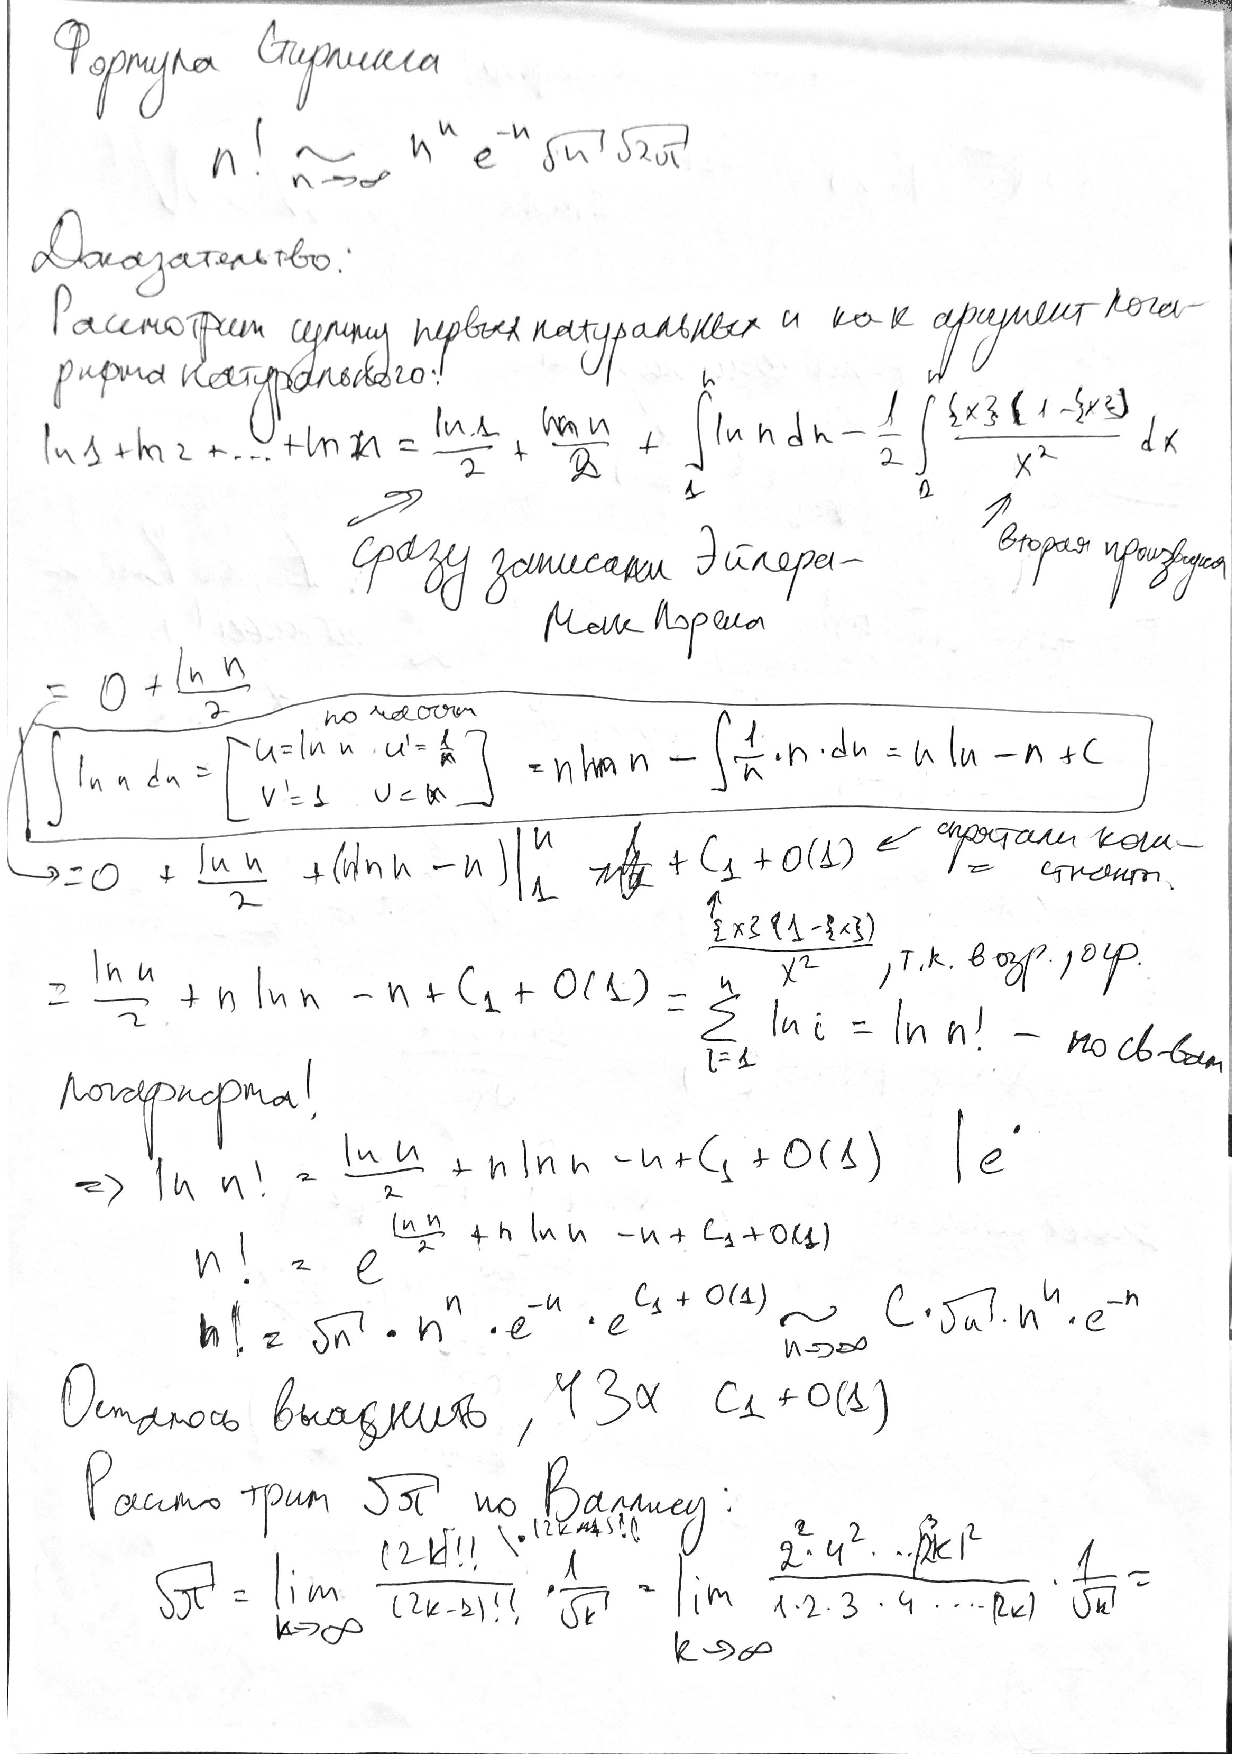
\includepdf[pages={-}]{../images/Stir.pdf}

\subsubsection{Признаки сравнения сходимости несобственного интеграла\texorpdfstring{$^2$}{}}
\subparagraph{Формулировка:}

$f, g$ --- допустимы на $[a, b)$

Если (хотя бы одно):
\begin{enumerate}
    \item $f \le g$ на $[a, b)$
    \item $\exists \lim_{x \rightarrow b - 0} {\frac{f(x)}{g(x)}} = l < \infty$
\end{enumerate}

То
\begin{enumerate}
    \item $\int_a^b g$ --- сходится $\Rightarrow \int_a^b f$ --- сходится
    \item $\int_a^b f$ --- расходится $\Rightarrow \int_a^b g$ --- расходится
\end{enumerate}

\subparagraph{Доказательство:}

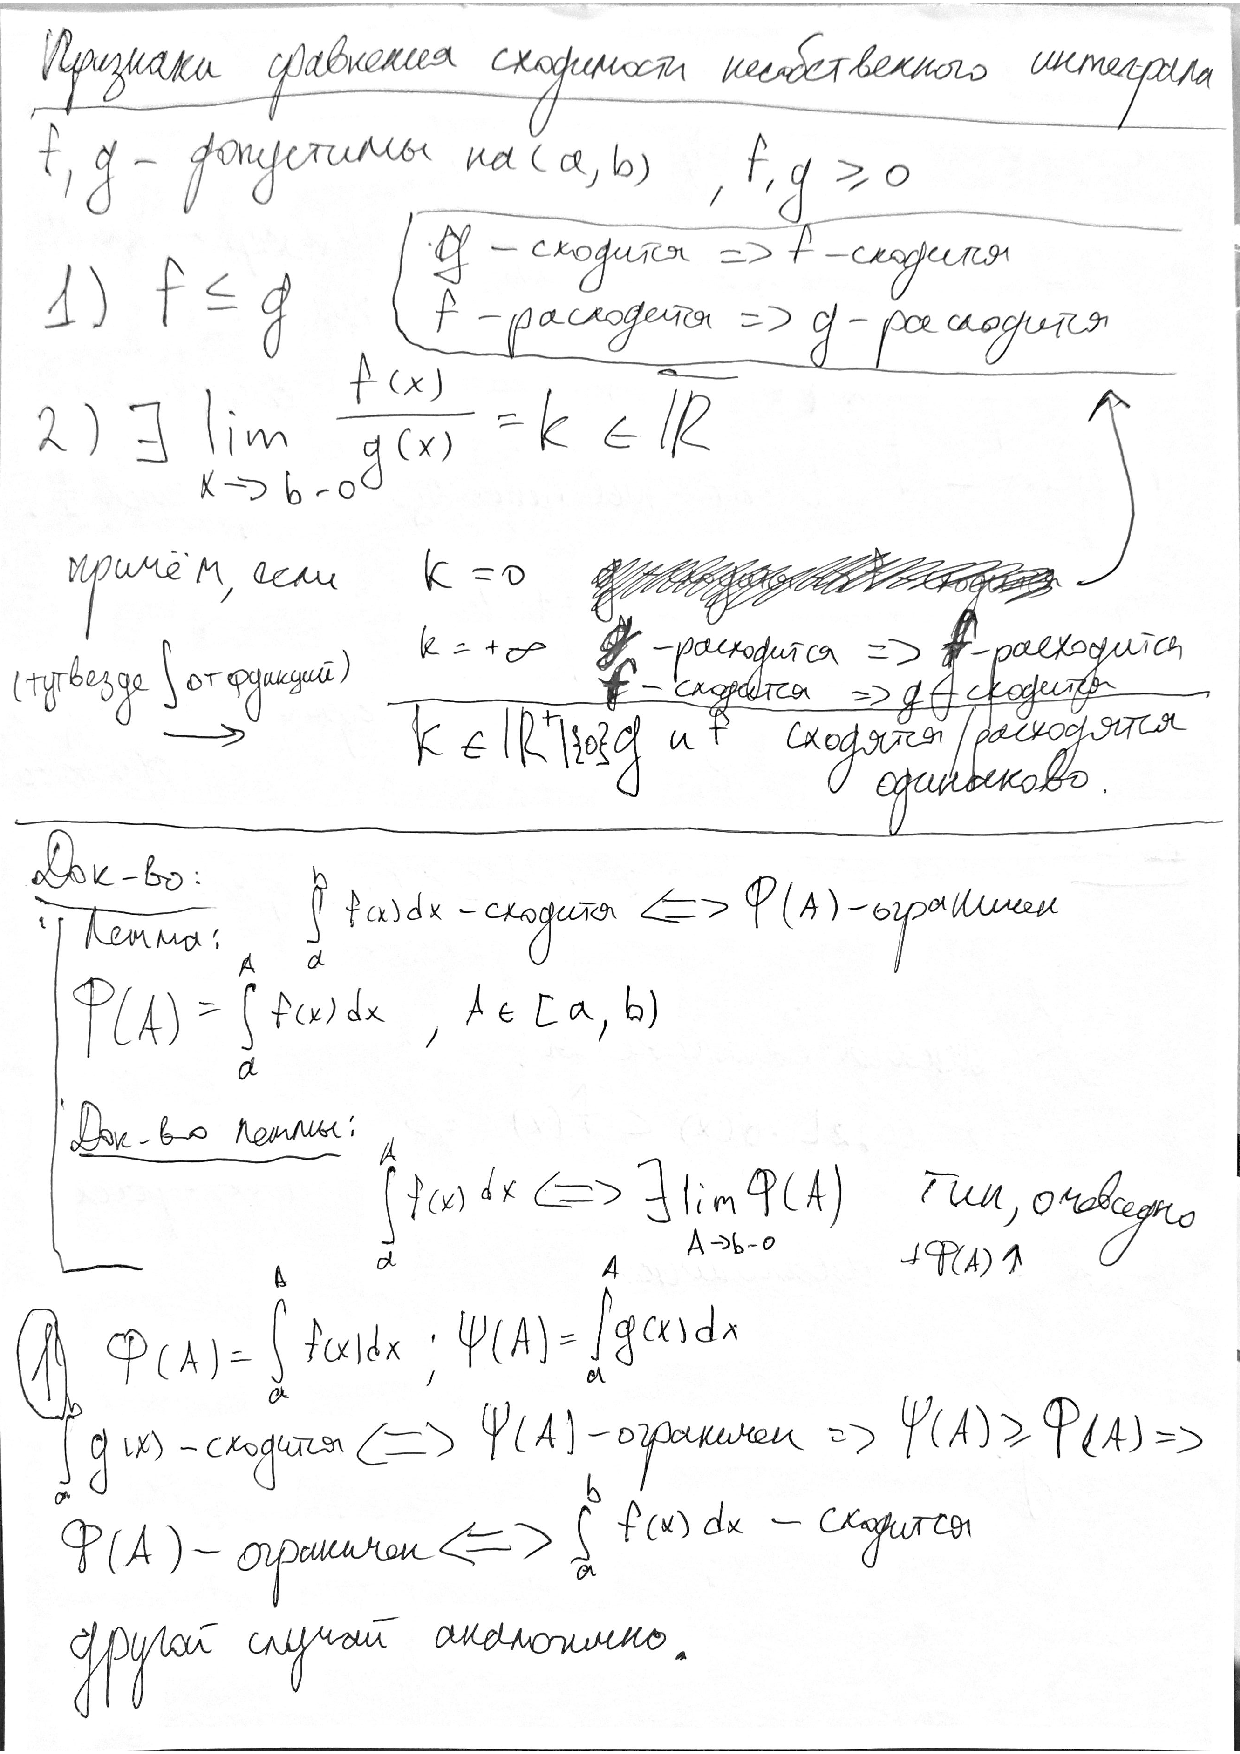
\includepdf[pages={-}]{../images/pris_srav_nesob.pdf}

\newpage

\subsection{Теоремы}
\subsubsection{Теорема о свойствах неопределённого интеграла\texorpdfstring{$^1$}{}}
\paragraph{Характеристика множества первообразных функции}
\subparagraph{Формулировка}

$F, f: \langle a, b\rangle \rightarrow \mathbb{R}, \forall x \in \langle a, b\rangle \quad F'(x) = f(x)$

Верны следующие утверждения:
\begin{enumerate}
    \item $\forall c \in \mathbb{R} \quad F + c$ --- первообразная $f$ на $\langle a, b \rangle$
    \item $\forall \overline{F}$ --- первообразная $f$ на $\langle a, b\rangle \quad \overline{F} = F + C$
\end{enumerate}

\subparagraph{Доказательство}
\begin{enumerate}
    \item Очевидно ($F'(c) = 0$)
    \item $(\overline{F} - F)' = 0, \int 0 \D x = C \Rightarrow \overline{F}$ отличается от $F$ на $C$
\end{enumerate}


\paragraph{Правила интегрирования}
\subparagraph{Формулировка}
$f, g$ имеют $F, G$ на $\langle a, b\rangle$

\begin{enumerate}
    \item $\int f + g = \int f + \int g$
    \item $\forall \alpha \in \mathbb{R} \quad \int \alpha f = \alpha \int f$
    \item Пусть $\phi: \langle c, d \rangle \rightarrow \langle a, b \rangle$. Тогда $(\int f(x) \D x)|_{x:= \phi(t)} = F(\phi(t)) + C = \int f(\phi(t))\phi'(t) \D t$
    \item $\forall \alpha, \beta \in \mathbb{R}, \alpha \ne 0 \quad \int f(\alpha x + \beta) \D x = \frac{1}{\alpha}F(\alpha x + \beta)$
    \item $f, g$ дифференцируемы. $\exists \int fg' \Rightarrow \exists \int f'g = fg - \int fg'$
    
    Пример: $\int \ln x \D x = \int 1 \cdot \ln x \D x$. Тогда $f' = 1 \Rightarrow f = x, g = \ln x \Rightarrow g' = \frac{1}{x}$. $\int 1 \cdot \ln x \D x = x \cdot \ln x - \int x \cdot \frac{1}{x} \D x = x\ln x - x + C$ 
\end{enumerate}

\subparagraph{Доказательство}
\begin{enumerate}
    \item $(F + G)' = F' + G' = f+g$
    \item $(\alpha F)' = \alpha f$
    \item $(F(\phi(t)))' = f(\phi(t)) \cdot \phi'(t)$
    \item $\int f(\alpha x + \beta) \D x = \int \frac{f(z) \D z}{(\alpha x + \beta)'} = \frac{1}{\alpha}F(\alpha x + \beta)$
    \item $(fg)' = f'g + fg' \Rightarrow (fg)' - fg' = f'g$. По арифметическим свойствам $\int f'g = \int (fg)' - \int fg' = fg - \int fg'$
\end{enumerate}



\subsubsection{Правило Лопиталя\texorpdfstring{$^2$}{}}

\paragraph{Лемма об ускоренной сходимости}
\subparagraph{Формулировка}

$f, g: D \rightarrow \mathbb{R}, D \subset \overline{\mathbb{R}}, a$ --- предельная точка $D, a \in \overline{\mathbb{R}}$.

$\exists \dot{V}_a : f, g \neq 0$ на $\dot{V}_a \cap D, \lim_{x \rightarrow a}{f(x)} = 0, \lim_{x \rightarrow a}{g(x)} = 0$

\paragraph{Правило Лопиталя}
\subparagraph{Формулировка:}

$f, g: (a, b) \rightarrow \mathbb{R}, a \in \overline{\mathbb{R}}$

$f, g$ --- дифф., $g^\prime \neq 0$ на $(a, b)$

Если:
\[\exists \lim_{x \rightarrow a + 0}{\frac{f^\prime(x)}{g^\prime(x)}} = L \text{ и } \frac{f(x)}{g(x)} \in \left\{\frac{0}{0}, \frac{\infty}{\infty}\right\}\]

Тогда: 
\[\lim_{x \rightarrow a + 0}{\frac{f(x)}{g(x)}} = L\]

\subparagraph{Доказательство:}

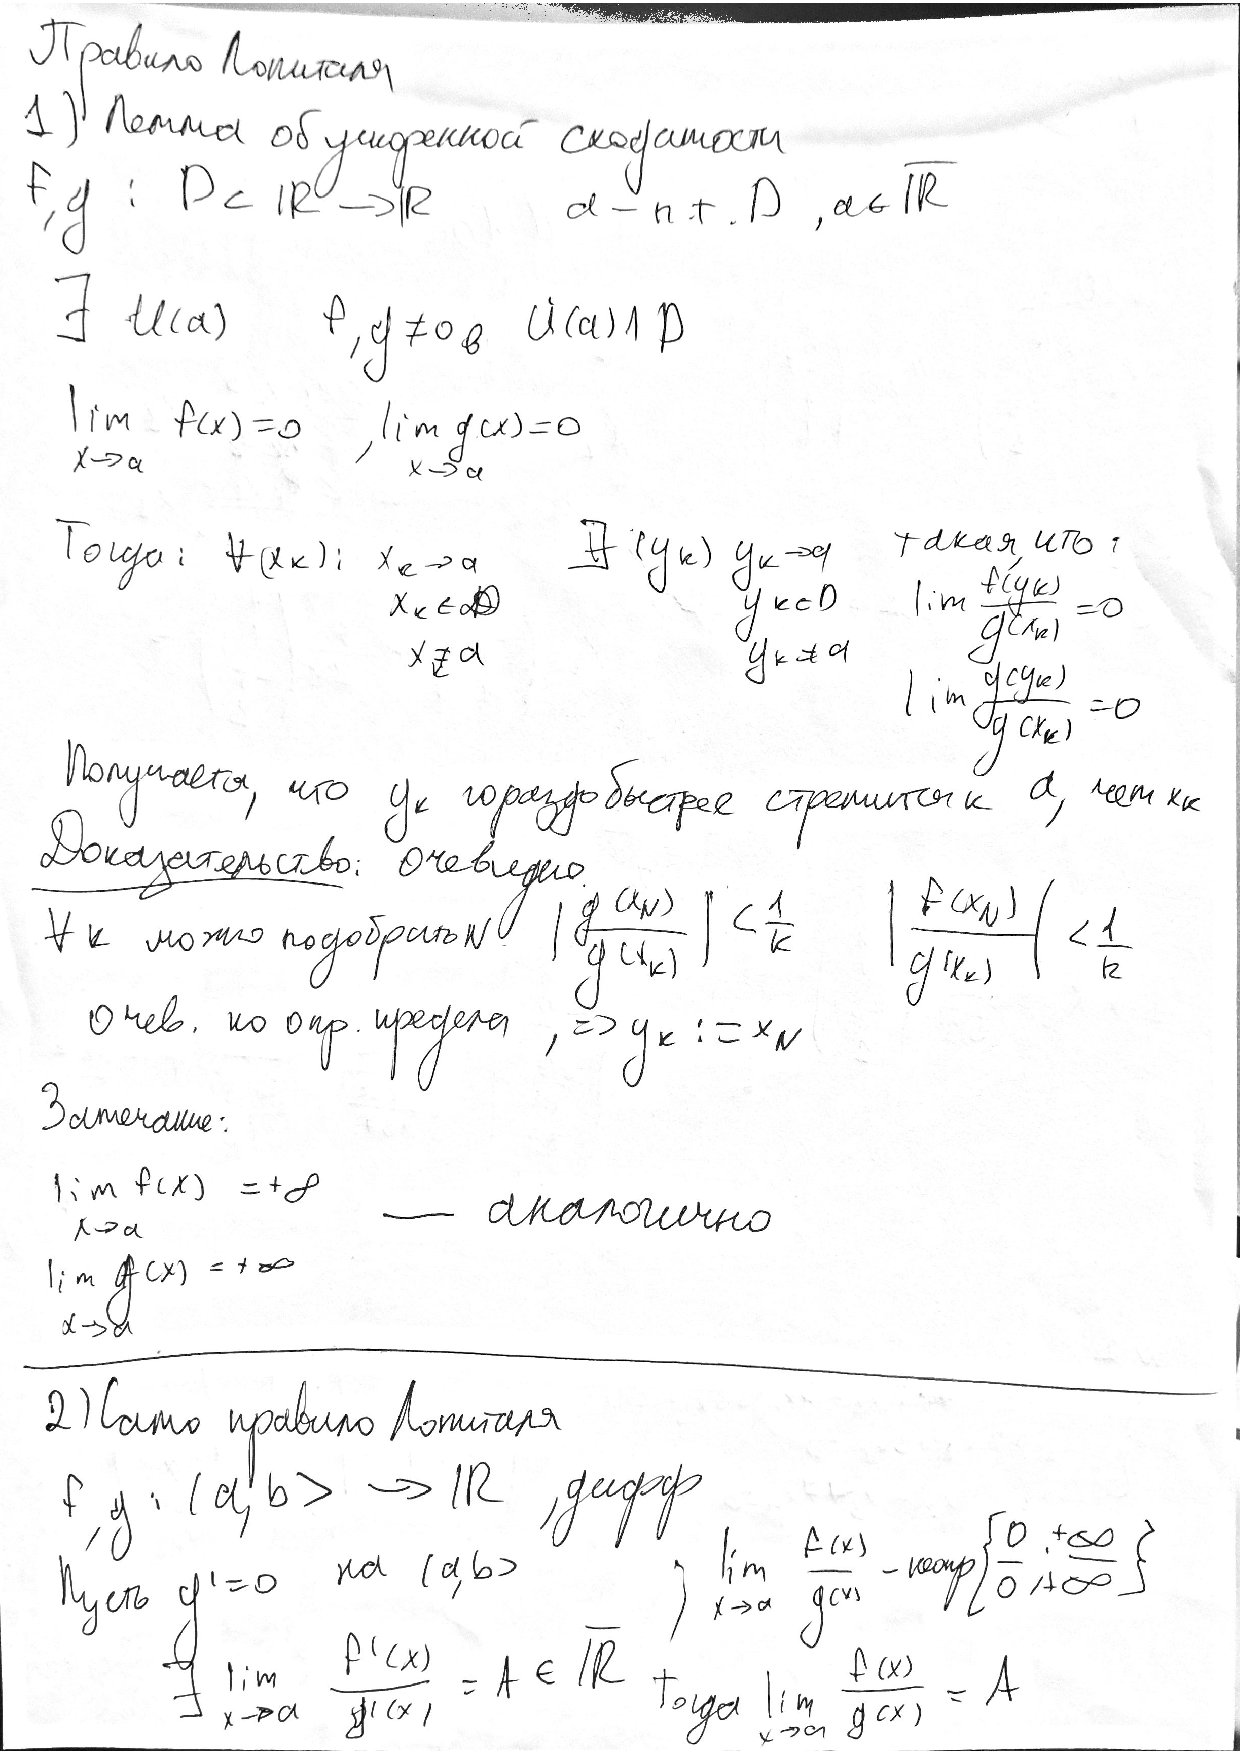
\includepdf[pages={-}]{../images/Lopit.pdf}

\subsubsection{Теорема Штольца\texorpdfstring{$^1$}{}}
\paragraph{Лемма о смешной сумме}
Ну что вы хотели, КПК же
\subparagraph{Формулировка}
$$
s < \frac ab< t
$$
$$
s < \frac c d < t
$$
$$
s < \frac {a+c}{b+d} < t
$$
\subparagraph{Доказательство}
Упражнение \Smiley

\subparagraph{Формулировка}
$x_n, y_n$ --- вещественные последовательности, $x_n, y_n \underset{\text{монотонно}}{\rightarrow} 0$

$$
\lim \frac{x_{n+1} - x_{n}}{y_{n+1} - y_n} = \lim \frac{x_n}{y_n}
$$

\subparagraph{Доказательство}
$\rhd$
Nota bene: Вообще мы тут рассматриваем только положительные числа, т.к. вышеупомянутая лемма вроде как работает только там. Но тут не должно быть проблем с сохранением общности, так что пофиг.

$$
\lim \frac{x_{n+1} - x_{n}}{y_{n+1} - y_n} = c \Rightarrow \forall \varepsilon > 0 \exists N: \forall N_1 > N, \forall n > N_1 \quad c-\varepsilon < \frac{x_{N_1+1} - x_{N_1}}{y_{N_1+1} - y_{N_1}} < c + \varepsilon
$$
Тут трюк такой: поскольку данное определение верно для всех $N_1 > N$, то мы можем продолжать расписывать такие неравенства до бесконечности (то есть рассмотреть $x_{N_1 + 2} - x_{N_1+1}$ и так далее. Давайте применим лемму о смешной сумме и сложим этот ряд неравенств. У нас всё, очевидно, сократится, кроме крайних членов:
$$
c-\varepsilon < \frac{x_{n} - x_{N_1}}{y_{n} - y_{N_1}} < c + \varepsilon
$$
Где $n \rightarrow \infty$. Ну а по определению предела, $x_n \rightarrow 0$, ровно как и $y_n$. Тогда их можно опустить в предельном переходе: 
$$
c-\varepsilon < \frac{y_{N_1}}{y_{N_1}} < c + \varepsilon
$$
$\lhd$

\subsubsection{Теорема Барроу\texorpdfstring{$^1$}{}}
\paragraph{Интеграл с переменным верхним пределом}
$f\in C[a, b], \phi: [a, b] \rightarrow \mathbb{R}$
Обозначим его за 
$$
\phi(x) = \int\limits_a^x f(x) 
$$

\subparagraph{Формулировка}
$$
\forall x\in [a, b] \quad \phi'(x) = f(x)
$$
Вот это прикол! Взяли какие-то странные интегралы, которые определены как какая-то недоплощадь, ещё и сделали область интегрирования переменной. А получили (внезапно) аж первообразную! 

\subparagraph{Доказательство}

Давайте распишем производную этой непонятной функции:
$$
\phi'(x) = \lim_{y\rightarrow x+0}\frac{\phi(y)-\phi(x)}{y-x} = \lim_{y\rightarrow x+0}\frac{\int\limits_a^y f - \int\limits_a^x f}{y-x} = \lim_{y\rightarrow x+0}\frac{\int\limits_x^y f}{y-x} \underset{\text{Теорема о среднем}}{=}
$$
$$
=\lim_{y\rightarrow x+0}f(c), c \in [x, y] \underset{\text{Наконец-то предельный переход}}{\longrightarrow} f(x)
$$

\subsubsection{Интегральное неравенство Чебышева. Неравенство для сумм\texorpdfstring{$^2$}{}}

\subparagraph{Формулировка}

\textit{ВИНОГРАДЫЧ}

$f, g : \left[a, b\right] \rightarrow \mathbb{R}$, причём $f$ --- возрастает, а $g$ --- убывает.

Тогда:

\[\frac{1}{b - a}\int_a^b{fg} \le \left(\frac{1}{b - a} \int_a^bf\right) \cdot \left(\frac{1}{b - a} \int_a^bg\right)\]


\textit{КОХАСЬ}

$f, g : \left[a, b\right] \rightarrow \mathbb{R}$, монотонны \textsc{одинаково}

Let $I_f = \frac{\int_a^b{f}}{b - a}$

Тогда:

\[ I_f \cdot I_g \le I_{fg}\]


\subparagraph{Доказательство}
$\rhd$

$\forall x, y \in [a, b] : \left(f(x) - f(y)\right)\left(g(x) - g(y)\right) \ge 0$, так как монотонны одинаково. 

Раскрываем скобки:

$f(x)g(x) - f(x)g(y) - f(y)g(x) + f(y)g(y) \ge 0$

Интегрируем по $y$ на промежутке $[a, b]$ и делим на $(b - a)$ 

$f(x)g(x) - I_fg(x) - f(x)I_g + I_fg \ge 0$

Интегрируем по $x$ на промежутке $[a, b]$ и делим на $(b - a)$

$I_{fg} - I_fI_g - I_fI_g + I_{fg} \ge 0$

$I_fI_g \le I_{fg}$

$\lhd$


\subparagraph{Формулировка}

\textit{ВИНОГРАДЫЧ}

$n \in \mathbb{N}; a, b \in \mathbb{R}^n$, причём $a_1 \le a_2 \le \ldots \le a_n$ и $b_1 \ge b_2 \ge \ldots \ge b_n$

Тогда:

\[\frac{1}{n}\sum_{k = 1}^n{a_kb_k} \le \left(\frac{1}{n}\sum_{k = 1}^n{a_k}\right) \cdot \left(\frac{1}{n}\sum_{k = 1}^n{b_k}\right)\]

\textit{КОХАСЬ}

$n \in \mathbb{N}; a, b \in \mathbb{R}^n$, причём $a_1 \le a_2 \le \ldots \le a_n$ и $b_1 \le b_2 \le \ldots \le b_n$

Тогда:

\[\left(\frac{1}{n}\sum_{k = 1}^n{a_k}\right) \cdot \left(\frac{1}{n}\sum_{k = 1}^n{b_k}\right) \le \frac{1}{n}\sum_{k = 1}^n{a_kb_k} \]


\subparagraph{Доказательство}

$\rhd$

Возьмём т.н. кусочно-постоянные функции $f, g: [0, 1] \rightarrow \mathbb{R}$, которые разбиты на $n$ кусочков, и $\left(\frac{k - 1}{n}, \frac{k}{n}\right)$-й кусочек равен $a_k$ и $b_k$ соответственно. Тогда просто запишем стандартное неравенство Чебышева и у нас всё получится! (на разрывы в конечном числе точек пофигу).

$\lhd$


\subsubsection{Свойства определенного интеграла: линейность, интегрирование по частям, замена переменных\texorpdfstring{$^2$}{}}

\paragraph{Линейность}

\[\int_a^b{\alpha f(x)} = \alpha \int_a^b{f(x)}\]
\[\int_a^b{f(x) + g(x)} = \int_a^b{f(x)} + \int_a^b{g(x)}\]


\paragraph{Интегрирование по частям}

\[\int_a^b{fg^\prime} = fg|_a^b - \int_a^b{gf^\prime}\]


\paragraph{Замена переменных}

\[\int_\alpha^\beta{f(\phi(x))\phi^\prime(x)} = \int_{\phi(\alpha)}^{\phi(\beta)}{f}\]

\paragraph{Доказательство}

Всё выводится из таких же свойств неопределённого интеграла

\subsubsection{Иррациональность числа пи\texorpdfstring{$^2$}{}}

Let $H := \frac{1}{n!}\int_{-\frac{\pi}{2}}^{\frac{\pi}{2}}{\left(\frac{\pi^2}{4} - t^2\right)^n\cos t dt} = \ldots$

Проинтегрируем по частям:

$u = \left(\frac{\pi^2}{4} - t^2\right)^n \Rightarrow du = -2nt\left(\frac{\pi^2}{4} - t^2\right)^{n - 1}dt$

$dv = \cos t dt \Rightarrow v = \sin t$

Следовательно, $\ldots = \frac{1}{n!}\left(\frac{\pi^2}{4} - t^2\right)\sin t|_{-\frac{\pi}{2}}^{\frac{\pi}{2}} + \frac{2}{(n - 1)!}\int_{-\frac{\pi}{2}}^{\frac{\pi}{2}}{t\sin t \left(\frac{\pi^2}{4} - t^2\right)^{n - 1}dt} = \ldots$ (причём слагаемое с синусом занулится)

Опять проинтегрируем по частям:

$u = t\left(\frac{\pi^2}{4} - t^2\right)^{n - 1} \Rightarrow du = \left(\left(\frac{\pi^2}{4} - t^2\right)^{n - 1} - 2t^2(n - 1)\left(\frac{\pi^2}{4} - t^2\right)^{n - 2}\right)dt$

$dv = \sin t dt \Rightarrow v = -\cos t$

Поработаем с $du$, приплюсуем и вычтем $2(n - 1)\frac{\pi^2}{4}\left(\frac{\pi^2}{4} - t^2\right)^{n - 2}$ и вынесем $2(n - 1)\left(\frac{\pi^2}{4} - t^2\right)^{n - 2}$ у минусового слагаемого в $du$ и плюсового $2(n - 1)\frac{\pi^2}{4}\left(\frac{\pi^2}{4} - t^2\right)^{n - 2}$:

$du = \left( 2(n - 1)\left( \frac{\pi^2}{4} - t^2\right)^{n - 2}\left(\frac{\pi^2}{4} - t^2\right) + \left(\frac{\pi^2}{4} - t^2\right)^{n - 1} - 2(n - 1)\frac{\pi^2}{4}\left(\frac{\pi^2}{4} - t^2\right)^{n - 2}\right)dt$

$= \left((2n - 1)\left(\frac{\pi^2}{4} - t^2\right)^{n - 1} - (n - 1)\frac{\pi^2}{2}\left(\frac{\pi^2}{4} - t^2\right)^{n - 2}\right)dt$

$\ldots = 0 + \frac{2}{(n - 1)!}t\left(\frac{\pi^2}{4} - t^2\right)^{n - 1}(-\cos t)|_{-\frac{\pi^2}{4}}^{\frac{\pi^2}{4}} + \frac{2}{(n -1)!}\left((2n - 1)\left(\frac{\pi^2}{4} - t^2\right)^{n - 1} - (n - 1)\frac{\pi^2}{2}\left(\frac{\pi^2}{4} - t^2\right)^{n - 2}\right)\cos tdt$

$= (4n - 2)H_1 - \pi^2H_2$


\subparagraph{Формулировка}

Число $\pi$ --- иррационально.

\subparagraph{Доказательство}

$H_0 = 2, H_1 = \ldots [\text{ по частям }] = 4$

$H_n = (\ldots)H_1 + (\ldots)H_0 = P_n(\pi^2)$ --- многочлен от $\pi^2$ степени $\le n$.

Почему? Ну типа мы взяли произвольное $n$, и посчитали для него $H_n$, и по рекуррентной формуле просто раскрыли всё до примитивов $(H_0, H_1)$  получили в конечном итоге огромный многочлен, зависящий от $\pi^2$.

Пусть $\pi^2 = \frac{p}{q}$ (рациональное)

$q^{n}P_n(\frac{p}{q}) = $ целое число (у нас огромный многочлен степени не больше $n$, в котором переменные $= \pi^2 = \frac{p}{q}$) $ = q^{n}H_n > 0$ (интеграл положителен на нашем интервале) $\Rightarrow q^{n}H_n \ge 1$ (так как интеграл положительный, $q^n$ --- целое, произведение тоже целое, а значит минимальное положительное целое --- 1)

$1 \le \frac{q^{n}}{n!}\int_{-\frac{\pi}{2}}^{\frac{\pi}{2}}{\left(\frac{\pi^2}{4} - t^2\right)^n\cos t dt} \le \frac{q^{n}}{n!}4^n\pi \rightarrow_{n \rightarrow \infty} 0$

Противоречие!

\subsubsection{Компактность и конечные эпсилон-сети\texorpdfstring{$^2$}{}}

\paragraph{Определения}

\begin{enumerate}
    \item Множество $N \subset X$ называется $\varepsilon$-сетью для $D$, если $\varepsilon > 0 \dbl \forall x \in D \exists y \in N \quad \rho(x, y) < \varepsilon$
    \item Множество $D$ --- сверхограниченное в $X$, если $\forall \varepsilon > 0 \exists$ конечная $\varepsilon$-сеть
\end{enumerate}

\paragraph{Свойства}

\begin{enumerate}
    \item $D\text{ --- сверхограниченно в }X \Leftrightarrow D\text{ --- сверхограниченно в себе}$
    
    \textbf{Доказательство:}
    $\rhd$
    
    $\Leftarrow$ ОЧЕВИДНО.
    
    $\Rightarrow$ Отметим $\{x_1, x_2, \ldots, x_n\} $ --- $ \frac{\varepsilon}{2}$ сеть в $X$. Теперь в каждом шарике $B(x_i, \frac{\varepsilon}{2})$ берём $y_i \in D$, если такая есть. Вуаля, $\{y_1, \ldots, y_{m \le n}\}$ --- $\varepsilon$-сеть для $D$.
    
    $\lhd$

    \item $\text{Сверхограниченность сохраняется при равномерно непрерывном отображении}$ \[\forall \varepsilon > 0 \exists \delta > 0 \forall u, v \in X: \rho(u, v) < \delta \dbl \rho(f(u), f(v)) < \varepsilon; f(\delta\text{-сети}) = \varepsilon\textit{-сеть}\]
    
    \textbf{Доказательство:}
    $\rhd$
    
    Возьмём $\delta$ из условия, выберем конечную $\delta$-сеть $N$ для $D$. Тогда, нам необходимо узнать, что при $E = f(D)$, $y = f(x)$, $E$ --- сверхорганиченно. Давайте возьмём любую точку $x$, найдём ближайшую $x_i$ из $D$ и посмотрим $f(x_i)$. Окажется, что $\rho(y, f(x_i)) < \varepsilon$. Вы скажете --- а почему??? Да всё просто, по равномерной непрерывности!
    
    $\lhd$

    
    \item $D\text{ --- сверхограниченно }\Rightarrow Cl(D)\text{ --- сверхограниченно}$
    
    \textbf{Доказательство:}
    $\rhd$
    
    $N$ --- конечная $\varepsilon$-сеть.
    
    $\forall x \in D \exists y \in N : \rho(x, y) < \varepsilon$
    
    Тогда:
    
    $\forall x \in Cl(D) \exists y \in N : \rho(x, y) \le \varepsilon$
    
    Возьмём $a \in D, a_i \rightarrow b (b \in Cl(D))$. Покрасим эту бесконечную последовательность в конечное число цветов, следовательно существует подпоследовательность одинакового цвета $a_{n_k}$. Следовательно, $a_{n_k} : \exists x_i \in N : \rho(a_{n_k}, x_i) < \varepsilon \ldots$ (предельный переход) $\rho(b, x_i) \le \varepsilon$. Получается, что мы получили т.н. $2\varepsilon$-сеть, типа, типа эпсилон надо взять чуть-чуть побольше.
    
    $\lhd$

    
    \item $D\text{ --- сверхограниченно }\Leftrightarrow \forall\text{ последовательность из $D$ содержит фундаментальную подпоследовательность}$
    
  \textbf{Доказательство:}
    $\rhd$
    
    $\Rightarrow$
    
    $\{y_n\}$ --- последовательность из $D$. Зафиксируем $\varepsilon = 1 : \{x_1, \ldots, x_n\}$. Логично, что в одном из шаров $B(x_i, \varepsilon)$ --- содержится бесконечно много элементов последовательности. Далее будем рассматривать только те элементы последовательности, которые внутри шара.
    
    Зафиксируем $\varepsilon = \frac{1}{2} : \{\hat{x}_1, \ldots, \hat{x}_n\}$. Логично, что в одном из шаров $B(\hat{x}_i, \varepsilon = \frac{1}{2})$ --- содержится бесконечно много элементов последовательности. Далее будем рассматривать только те элементы последовательности, которые внутри шара.
    
    И так далее!
    
    А почему же построенная система из под-шаров будет являться фундаментальной последовательностью? Да дело в том, что по определению фундаментальной последовательности, начиная с какого-то номера все элементы подпоследовательности будут лежать сколь угодно близко. А мы тут делаем ровно это --- просто берём нужный эпсилон и строим шары.
    
    $\Leftarrow$
    
    Очевидно. \Smiley
    
    Так как если нет конечной $\varepsilon$-сети, то $\exists \{x_n\}$ в $D : \rho(x, x_i) \ge \varepsilon \Rightarrow$ нельзя выбрать фундаментальную подпоследовательность. 

    $\lhd$
\end{enumerate}

\paragraph{Теорема}

\subparagraph{Формулировка:}

$(X, \rho)$ --- метрическое пространство, $X$ --- полное, $D \subset X$

Тогда эквивалентно:

\begin{enumerate}
    \item $D$ --- компактно.
    \item $D$ --- сверхограничено, замкнуто.
\end{enumerate}

\subparagraph{Доказательство: }
(в метрическом пространстве)

$X$ --- компактно $\Leftrightarrow X$ --- секвенциально компактно

$\rhd$

$\Rightarrow$

Полноту получаем автоматически. Если $\exists$ фундаментальная последовательность $\{y_n\}$, не имеющая предела, то из секвенциальной компактности $X$ следует, что существует сходящаяся подпоследовательность $\{x_{n_k}\}$

Допустим, что $X$ --- не сверограниченно $\Rightarrow \exists \{x_n\}$, из которой нельзя извлечь фундаментальную подпоследовательность, однако, это противоречит секвенциальной компактности (сх. подпосл. фундаментальна).

$\Leftarrow$

Сверхограниченно $\Rightarrow$ из любой последовательности можно извлечь фундаментальную $\Rightarrow$ она сходится (в силу полноты) $\Rightarrow$ оно секвенциально компактно $\Rightarrow_{\text{в } X}$ компактно.

$\lhd$

\subsubsection{Площадь криволинейного сектора: в полярных координатах и для параметрической кривой\texorpdfstring{$^2$}{}}

\subparagraph{Формулировка:}

$f(\varphi): [0, 2\pi] \rightarrow [0, \infty)$ --- непрерывная функция.

$\Phi([\alpha, \beta]) = S_{\text{сектора } [\alpha, \beta]}, \dbl g(\phi) = \frac{r^2(\phi)}{2}$

\[\Phi([\alpha, \beta]) = \int_\alpha^\beta{g(\phi)d\phi} = \frac{1}{2}\int_\alpha^\beta{r^2(\phi)d\phi}\]

Для параметрической:

\[S =  \frac{1}{2}\int_{t_\alpha}^{t_\beta}{(y^\prime(t)x(t) - x^\prime(t)y(t))dt}\]

\subparagraph{Доказательство:}

$\rhd$

Во первых, возьмём функцию промежутка (угла) $\Phi([\alpha, \beta]) = S_{\text{сектора }[\alpha, \beta]}$ и 'функцию' $g(\varphi) = r^2(\varphi)/2$. Если мы докажем, что $g$ --- плотность $\Phi$, то теореме о вычислении АФП по плотности у нас всё будет супер.

Заметим, что кусочек круга (круговой сектор) имеет площадь $\frac{1}{2}(\beta - \alpha) r^2$ (цитата: \textit{школьная формула}, а вообще, это достаточно логично, мы выбираем кусок круга, ограниченный двумя углами, причём мы смотрим внутри одной четверти, поэтому делим обычную площадь $\pi r^2$ на 4). Также, достаточно очевидно, что если мы на нашем промежутке (любом) найдём минимум и максимум функции, то \textit{сектор}(минимума) $\subset$ \textit{сектор}(функции) $\subset$ \textit{сектор}(максимума). Ура! 

\[\frac{1}{2}(\beta - \alpha) \min{r^2(\varphi)}_{\varphi \in [\alpha, \beta]} \le \Phi([\alpha, \beta]) \le \frac{1}{2}(\beta - \alpha) \max{r^2(\varphi)}_{\varphi \in [\alpha, \beta]}\]

Тогда по определению, $g$ --- плотность $\Phi$.

$\lhd$

Теперь просто переведём для параметрической формулы. $r(\varphi) = \sqrt{x^2(t) + y^2(t)}$. Также, проведём замену переменный в интеграле,
$\phi(t) = \arctan {\frac{y(t)}{x(t)}}$

\[\Phi([\alpha, \beta]) = \frac{1}{2}\int_\alpha^\beta{r^2(\varphi)d\varphi} = \frac{1}{2}\int_{\phi(\alpha)}^{\phi(\beta)}{r^2(\varphi)\phi^\prime(t)dt} = \frac{1}{2}\int_{\phi(\alpha)}^{\phi(\beta)}{(x^2(t) + y^2(t))\left(\arctan {\frac{y(t)}{x(t)}}\right)^\prime dt} = \]

\[ = \frac{1}{2}\int_{\phi(\alpha)}^{\phi(\beta)}{(x^2(t) + y^2(t))\left(\frac{1}{1 + \left(\frac{y(t)}{x(t)}\right)^2}\right)\left(\frac{y(t)}{x(t)}\right)^\prime dt} = \] 

\[ = \frac{1}{2}\int_{\phi(\alpha)}^{\phi(\beta)}{(x^2(t) + y^2(t))\left(\frac{x^2(t)}{x^2(t) + y^2(t)}\right)\left(\frac{y^\prime(t)x(t) - x^\prime(t)y(t)}{x^2(t)}\right) dt} = \]

\[ = \frac{1}{2}\int_{\phi(\alpha)}^{\phi(\beta)}{y^\prime(t)x(t) - x^\prime(t)y(t) dt} \]


\subsubsection{Изопериметрическое неравенство\texorpdfstring{$^2$}{}}
\subparagraph{Формулировка:}

$G \subset \mathbb{R}^2$ --- замкнуто и ограничено.

$\text{diam } G = \sup{\{\rho(x, y) : \forall x, y \in G\}} \le 1$

$\sigma(G) \le \frac{\pi}{4}$

\subparagraph{Доказательство:}

$\rhd$

Рассмотрим наше множество в 1 четверти декартовой системы координат:

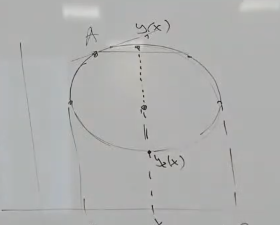
\includegraphics[]{../images/isoperim1.png}

Рассмотрим его над- и под- графики. Заметим, что эти функции почти дифференцируемые (?). Возьмём какую-нибудь производную (касательную) и примем её за Oy:

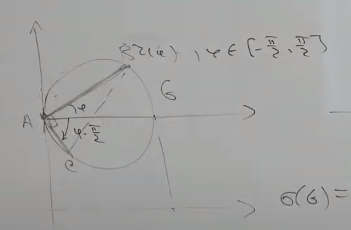
\includegraphics[]{../images/isoperim2.png}

Теперь можем ввести функцию для площади сектора $r(\varphi) \Rightarrow \frac{1}{2}\int_{-\frac{\pi}{2}}^{\frac{\pi}{2}}{r^2(\varphi)d\varphi}$.

Возьмём какой-нибудь уголок $\varphi$, и отложим от него 90 градусов вниз, тем самым получим с Ox новый угол $\varphi - \frac{\pi}{2}$. Теперь делаем финт ушами, делим наш интеграл на промежуток до 0 и после, в части от $-\frac{\pi}{2}$ до 0 заменяем переменную на $\alpha = \varphi - \frac{\pi}{2}$ и потом грациозно меняем $\alpha$ на $\varphi$, так как нам по барабану, как называется переменная. Суммируем интегралы:

\[\frac{1}{2}\int_0^{\frac{\pi}{2}}{r^2(\varphi) + r^2(\varphi - \frac{\pi}{2}) d\varphi}\]

А теперь самое интересное. Посмотрим на отрезки $AB$ и $AC$, заметим, что это прямоугольный треугольник, и, соответственно, сумма их квадратов равна $BC$. А $BC \le \textsc{diag}(G) \le 1$, следовательно:

\[\frac{1}{2}\int_0^{\frac{\pi}{2}}{1 d\varphi} = \frac{\pi}{4}\]

$\lhd$

\subsubsection{Обобщенная теорема о плотности\texorpdfstring{$^1$}{}}
\subparagraph{Формулировка}
$\letus \phi: \segm \langle a, b \rangle \rightarrow \mathbb{R}$ --- аддитивная функция промежутка

$\letus f: \langle a, b \rangle \rightarrow \mathbb{R}$ --- непрерывна

$\letus \delta$ --- произвольный отрезок $\in \langle a, b \rangle$

$\letus m_\delta \le \inf_{x\in \delta}f(x)$, $M_\delta \ge \sup_{x\in \delta}f(x)$

\begin{enumerate}
    \item $m_\delta \cdot l_\delta \le \phi(\delta) \le M_\delta \cdot l_\delta$
    \item $\forall x \in \delta \quad m_\delta \le f(x) \le m_\delta$
    \item $\forall \delta \rightarrow [x, x] \quad M_\delta - m_\delta \rightarrow 0$
\end{enumerate}

Вот это ВСЁ должно выполняться. И тогда мы утверждаем, что верно: $\phi([p, q]) = \int_p^q f(x)\D x$. Это утверждение --- синоним того, что $f$ --- плотность $\phi$

\subparagraph{Доказательство}
$\rhd$

Для начала введём функцию, для которой потом будем пытаться доказать то, что она первообразная.

$\letus F(x) = 0$, если $x = p$ (отрезок $[p, p]$). $F(x) = \phi([p, x])$, если $x \in (p, q]$.

$\letus \delta = [x, y] \in [p, q]$

Идём просто по порядку нумерованных утверждений:
\begin{enumerate}
    \item Разделим всё на $l_\delta$. $m_\delta \le \frac{\phi(\delta)}{l_\delta} \le M_\delta$. Заметим, что $\phi(\delta) = F(y) - F(x)$, т.к. $\phi$ аддитивна.
    
    \item Заметили, что наши достижения из прошлого пункта и в этом зажаты в одном промежутке ($[m_\delta, M_\delta]$). Давайте этим воспользуемся и вычтем из первого второе: $|\frac{F(y) - F(x)}{l_\delta} - f(x)| \le M_\delta - m_\delta$.
    
    \item Возьмём достижение из прошлого пункта. Заметим, что $l_\delta = y - x$. А теперь давайте устремим $l_\delta$ в $0$. $\lim\limits_{y\rightarrow x} |\frac{F(y) - F(x)}{y - x} - f(x)| \le M_\delta - m_\delta$. Вспоминаем что мы писали в условии про 3 пункт, выясняется, что $M_\delta - m_\delta \rightarrow 0$, то есть всё это выражение стремится к 0. О БОЖЕ!!! Мы же получили ровно определение производной!
\end{enumerate}
$\lhd$


\subsubsection{Объём фигур вращения\texorpdfstring{$^1$}{}}
$\letus \delta = [p, q] \in \langle a, b \rangle$

$f: \langle a, b \rangle$ непрерывна (или кусочно-непрерывна, но там мы рассматриваем эти куски отдельно, ничего интересного)

$\letus \phi_x$ --- объём фигуры вращения $f$ относительно оси $x$ (получится криволинейная сосиска \Smiley)

$\letus \phi_y$ --- объём фигуры вращения $f$ относительно оси $y$ (получится бублик). Обращаем внимание, что радиус бублика в каждой точке вращения разный (чем дальше от оси, тем больше)

Утверждаем, что $\phi_x(\delta) = \pi \cdot \int_p^q f^2(x) \D x$. Вместо доказательств давайте разберёмся что откуда берётся: $\pi$ мы просто вынесли как константу, $\pi f^2(x)$ --- это площадь среза нашей колбасы в точке $x$. Ну и интегрируем её просто на нужном отрезке.

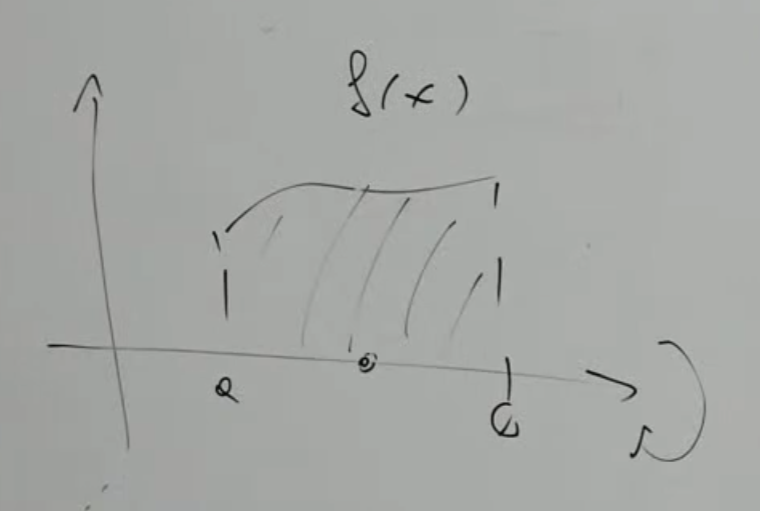
\includegraphics[]{rotate_x.png}

Далее, $\phi_y(\delta) = 2\pi \cdot \int_p^q x \cdot f(x) \D x$. Тут не всё так очевидно на первый взгляд. На самом деле, всё элементарно: $2\pi x$ --- это просто длина окружности в точке вращения. $f(x)$ же просто высота среза в этом месте. 

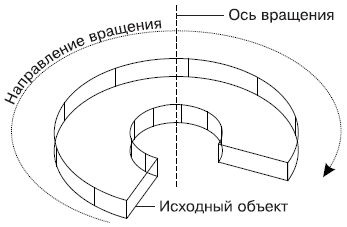
\includegraphics[]{rotate_y.png}


\subsubsection{Формула Тейлора с остатком в интегральной форме\texorpdfstring{$^1$}{}}
\subparagraph{Формулировка}
$f \in C^{n+1}(\langle a, b\rangle)$

$x, x_0 \in \langle a, b \rangle$

Тогда
$$
f(x) = f(x_0) + \frac{f'(x_0)}{1!}(x-x_0) + \frac{f''(x_0)}{2!}(x-x_0)^2 + \ldots + \frac{f^{(n)}(x_0)}{n!}(x-x_0)^n + \frac{1}{n!}\int_{x_0}^x (x-t)^n f^{(n+1)}(t)\D t
$$

\subparagraph{Доказательство}
$\rhd$

А получается это очень просто, по индукции.
База $n = 0$:
$$
f(x) = f(x_0) + \int_{x_0}^x f'(t) \D t
$$
Важно: чтобы такие трюки работали, производная должна существовать (по условию $f \in C^{n+1}$

Интегрируем по частям:
$\int 1 \D t = t + C = t - x = -(x - t)$
$$
\int_{x_0}^x f'(t) \D t = -(x - t) \cdot f'(t) + \int_{x_0}^x (x - t) \cdot f''(t) \D t
$$

Ещё раз:
$\int -(x - t) \D t = \frac{1}{2} -(x - t)^2$. Заметили, что степень будет каждую итерацию инкрементиться, а так же каждую итерацию будет появляться множитель--дробь с знаменателем $i$. Так, когда мы дойдём до $n$, эта часть будет равна $\frac{1}{n!} -(x-t)^n$
$\lhd$


\subsubsection{Вычисление длины гладкого пути\texorpdfstring{$^1$}{}}
\subparagraph{Формулировка}
$\letus \gamma: [a, b] \rightarrow \mathbb{R}^m$, $\gamma$ --- гладкий путь.
$$
l(\gamma) = \int\limits_a^b |\gamma'(t)| \D t
$$

Note: работает только когда $\gamma$ инъективен.

\subparagraph{Доказательство}
$\rhd$

$\letus [p, q] \in \segm[a, b]$

Введём функцию $\phi([p, q]) = l(\gamma|_{[p, q]})$. Заметим, что это аддитивная функция промежутка (по 2 аксиоме гладкого пути). Вспоминаем "Теорема о вычислении аддитивной функции промежутка по плотности". То есть мы уже можем сказать, что на всём $[a, b]$ длина считается через $\int\limits_a^b ||\gamma'(t)|| \D t$. Однако, нам надо доказать, что $||\gamma'(t)||$ --- плотность $\phi$.

Для этого нужно проверить 3 утверждения:

$M_i([p, q]) := \max_{t\in[p, q]} |\gamma_i'(t)|$
\begin{enumerate}
    \item $m_{[p, q]} \cdot l_{[p, q]} \le \phi([p, q]) \le M_{[p, q]} \cdot l_{[p, q]}$
    
    Введём $\overline{\gamma}: [p, q] \rightarrow \mathbb{R}^m \quad \overline{\gamma}(t) = M([p,q]) \cdot t$
    
    Введём носители путей $\gamma$ и $\overline{\gamma}$: $C_\gamma C_{\overline{\gamma}}$
    
    Заметим, что отображение $T: C_\gamma \rightarrow C_{\overline{\gamma}}$ --- растяжение, т.к. $\forall i, j \in [p, q] \quad \rho(\gamma(i), \gamma(j)) = \sqrt{\sum_{k=1}^m (\gamma_k(i) - \gamma_k(j))^2} \underset{\text{Т. Лагранжа}}{=} \sqrt{\sum_{k=1}^m (\gamma'_k(c_k) \cdot (j - i) )^2} \le |j-i| \cdot \sqrt{\sum_{i=1}^m M_i^2([p, q])} = |j - i| \cdot M_{[p, q]} = \rho(\overline{\gamma}(i), \overline{\gamma}(j))$
    
    А это ровно и обозначает то, что мы записали в условии: $\phi([p, q]) \le |j - i| \cdot M_{[p, q]}$.
    
    Для минимумов симметрично
    
    \item $\forall x \in [p, q] \quad m_{[p, q]} \le ||\gamma'(x)|| \le M_{[p, q]}$
    
    $\gamma'(x) = \sqrt{\sum_{i=1}^m (\gamma'_i(x))^2} \le M_{[p, q]}$, т.к. никакое $\gamma'_i(x)$ не может быть больше максимума на промежутке. Для минимума симметрично.
    
    \item $\forall x \in [p, q] \quad M_{[p, q]} - m_{[p, q]} \underset{q - p \rightarrow 0}{\rightarrow} 0$
    
    Поскольку все $\gamma'_i(x)$ непрерывны, то предел максимума на отрезке, стремящемся к нему будет равен самому $\gamma'_i(x)$. Таким образом, разность минимума и максимума $\rightarrow 0$ (из непрерывности $\gamma'$ и предыдущего утверждения)
\end{enumerate}

$\lhd$


\subsubsection{Свойства верхнего и нижнего пределов\texorpdfstring{$^1$}{}}
\subparagraph{Формулировка}
$\letus x_n$

Если ничего не написано про нижний предел, значит там всё работает аналогично.
\begin{enumerate}
    \item $\underline{\lim} x_n \le \overline{\lim} x_n$
    \item $\letus k_n \le x_n \quad \overline{\lim} k_n \le \overline{\lim} x_n$
    \item $\letus \lambda \ge 0 \quad \overline{\lim} (\lambda x_n) = \lambda \overline{\lim} x_n$
    \item $\overline{\lim} (-x_n) = -\underline{\lim} x_n$
    \item $\letus k_n \quad \overline{\lim} (x_n + k_n) \le \overline{\lim} x_n + \overline{\lim} k_n$\\
    $\underline{\lim} (x_n + k_n) \ge \underline{\lim}x_n + \underline{\lim}k_n$
    \item $\letus t_n \rightarrow l \in \mathbb{R} \quad \overline{\lim} (x_n + t_n) = \overline{\lim} (x_n) + l$
    \item $\letus t_n \rightarrow l > 0 \in \mathbb{R} \quad \overline{\lim} (t_n \cdot x_n) = l \cdot \overline{\lim} x_n$
\end{enumerate}

\subparagraph{Доказательство}
Тут я буду ссылаться на простейшие свойства из определения \nameref{ВНП}.
\begin{enumerate}
    \item Очевидно из свойства 2.
    
    \item $\overline{\lim} x_n = \sup(x_n, x_{n+1}, \ldots)$\\
    $\overline{\lim} k_n = \sup(k_n, k_{n+1}, \ldots)$. Следовательно, поскольку все элементы меньше, то и точная граница будет меньше. 
    
    \item Очевидно по той же логике. Если мы берём $\sup(\lambda x_n, \lambda x_{n+1}, \ldots) = \lambda \sup(x_n, x_{n+1}, \ldots)$
    
    \item Простая логика неравенств: $x < a \Rightarrow -x > -a$. $\sup(-x_n, -x_{n+1}, \ldots) = -\inf(x_n, x_{n+1}, \ldots)$
    
    \item Очевидно. Равенство достигается, когда последовательности положительны. В противном случае, одна может вычесть другую и вместо увеличения верхнего предела, он уменьшится.
    
    \item $\forall \varepsilon > 0 \exists N_0 : \forall k > N_0 \quad l - \varepsilon \le t_k \le l + \varepsilon$\\
    $l - \varepsilon + x_k \le t_k + x_k \le l + \varepsilon + x_k$\\
    $\sup x_k = y_N$. Возьмём $N > N_0$. Перейдём к $\sup$: $l - \varepsilon + y_N \le \sup(t_N + x_N, t_{N+1} + x_{N+1}, \ldots) \le l + \varepsilon + y_N$\\
    $y_N \rightarrow \overline{\lim}x_n, \sup(t_N + x_N, t_{N+1} + x_{N+1}, \ldots) \rightarrow \overline{\lim} (x_n + t_n)$\\
    $\overline{\lim}(x_n) + l - \varepsilon \le \overline{\lim} (x_n + t_n) \le \overline{\lim} (x_n) + l + \varepsilon$. А поскольку $\varepsilon \rightarrow 0$, мы его опускаем и получаем выражение из условия
    
    То есть что мы тут сделали: расписали предел $t_k$, прибавили к нему $x_k$, перешли к супремуму, устремили $N$ в бесконечность и сделали предельный переход, после которого всё превратилось в верхние пределы и сошлось.
    
    \item КПК не хочет доказывать \Smiley
\end{enumerate}


\subsubsection{Техническое описание верхнего предела\texorpdfstring{$^1$}{}}
\label{ТехВерхПредел}
\subparagraph{Формулировка}
$\letus x_n$
\begin{enumerate}
    \item $\overline{\lim} x_n = +\infty \Leftrightarrow x_n$ не ограничено сверху
    \item $\overline{\lim} x_n = -\infty \Leftrightarrow x_n \rightarrow -\infty$
    \item $\overline{\lim} x_n = l \in \mathbb{R} \Leftrightarrow $ \begin{enumerate}
        \item $\forall \varepsilon > 0 \exists N : \forall n > N \quad x_n < l + \varepsilon$
        \item $\forall \varepsilon > 0 \exists$ беск. число $n : x_n > l - \varepsilon$
    \end{enumerate}
\end{enumerate}

\subparagraph{Доказательство}
\begin{enumerate}
    \item Очевидно
    
    \item $\Rightarrow$\\ 
    Так же очевидно: $\sup(x_n, x_{n+1},\ldots) = -\infty$, а по свойству 2, $x_n \le y_n$.\\
    $\Leftarrow$\\
    Если $x_n$ стремится к $-\infty$, то $\forall E < 0 \exists N : \forall n > N \quad x_n < E \Rightarrow sup(x_n, x_{n+1}, \ldots) < E$
    
    \item $\Rightarrow$\\
    \begin{enumerate}
        \item По свойству 2, $x_n \le y_n$, а $y_n$ монотонно убывает и $y_n \rightarrow l$
        \item Очевидно из того факта, что последовательность $y_n$ имеет бесконечное количество элементов, при том, что $y_n \rightarrow l$. То есть мы можем брать бесконечное число элементов и получим выполнение условия.
    \end{enumerate}
    $\Leftarrow$\\
    $\forall \varepsilon > 0 \exists N : \forall n > N \quad x_n < l + \varepsilon, \forall \varepsilon > 0 \exists$ беск. число $n : x_n > l - \varepsilon$. Возьмём эти неравенства и перейдём к супремуму (который мы обозначаем как $y_n$:\\
    $l - \varepsilon \le y_n \le l + \varepsilon$. Верхняя оценка верна по умолчанию, а нижняя потому, что $y_n$ --- супремум, то есть ВЕРХНЯЯ граница.
\end{enumerate}


\subsubsection{Теорема о существовании предела в терминах верхнего и нижнего пределов\texorpdfstring{$^1$}{}}
\subparagraph{Формулировка}
$\overline{\lim}x_n = \underline{\lim}x_n \Leftrightarrow \exists \lim x_n$

\subparagraph{Доказательство}
$\Rightarrow$

$\underline{\lim}x_n$ это предел последовательности $z_m$, которая состоит из $\inf_{n\in [m, +\infty) \cap \mathbb{N}} x_n$. Очевидно, $z_n \le x_n$. Аналогичное верно для $\overline{\lim}x_n$ (пусть последовательность тут будет $k_n$). 

Соответственно, $z_n \le x_n \le k_n$. А поскольку $\overline{\lim}x_n = \underline{\lim}x_n$, то по теореме о двух городовых, $x_n$ имеет тот же предел.

$\Leftarrow$

$\overline{\lim}x_n = l \Rightarrow \forall \varepsilon > 0 \exists N : \forall n > N x_n < l + \varepsilon$. Заметим, что если мы сюда подставим определение предела последовательности по Коши, то это определение так же выполняется. Разумеется, в оба определения в качестве предела мы подставляем точку $l$ и видим, что ничего не нарушается ($\varepsilon$-окрестность точки $l$, в которой лежат все точки, начиная с $N$, гарантирует выполнение $x_n < l + \varepsilon$. Для нижнего предела всё то же самое, а поскольку точка у нас фиксирована, мы видим равенство верхнего и нижнего пределов.


\subsubsection{Теорема о характеризации верхнего предела как частичного\texorpdfstring{$^1$}{}}
\subparagraph{Формулировка}
$\overline{\lim}x_n = l \Rightarrow \exists \lim x_{n_k}=l$

\subparagraph{Доказательство}
Очевидно, чтобы такое доказать, надо предъявить подходящую подпоследовательность. По тех. определению верхнего предела, точка является предельной в последовательности, то есть мы можем сколько угодно приближать $\varepsilon$, в ней найдётся нужная точка.

$$
\forall k \in \mathbb{N} \exists n_k : l - \frac{1}{k} \le x_{n_k} \le l + \frac{1}{k}
$$

То есть грубо говоря, мы выдумали последовательность, которая стремится к $l$. Супремум является предельной точкой, а значит, мы можем приближать нашу последовательность в любом из супремумов (у нас же предел --- последовательность супремумов). Ну другими словами, это значит, что мы можем при всём этом сделать так, чтобы последовательность $n_k$ была возрастающей. И таким образом мы вытащили самую настоящую подпоследовательность, а значит нашли частичный предел, равный верхнему.

Ещё не забываем, что верхний предел может быть бесконечностью, но там всё очевидно. Выбираем подпоследовательность, стремящуюся в бесконечность. У нас последовательность не ограничена, а значит такой есть.

\subsubsection{Теорема о формуле трапеций, формула Эйлера--Маклорена\texorpdfstring{$^2$}{}}

\subparagraph{Формулировка (Теорема о формуле трапеций):}

$f \in C^2[a, b], \tau$ --- дробление, $\delta = \max(x_i - x_{i - 1})$

Тогда
\[\left|\int_a^b{f} - \sum{\frac{f(x_i) + f(x_{i - 1})}{2}(x_i - x_{i - 1})}\right| \le \frac{\delta^2}{8}\int_a^b{\left|f^{\prime\prime}\right|}\]

\subparagraph{Доказательство (Теорема о формуле трапеций):}

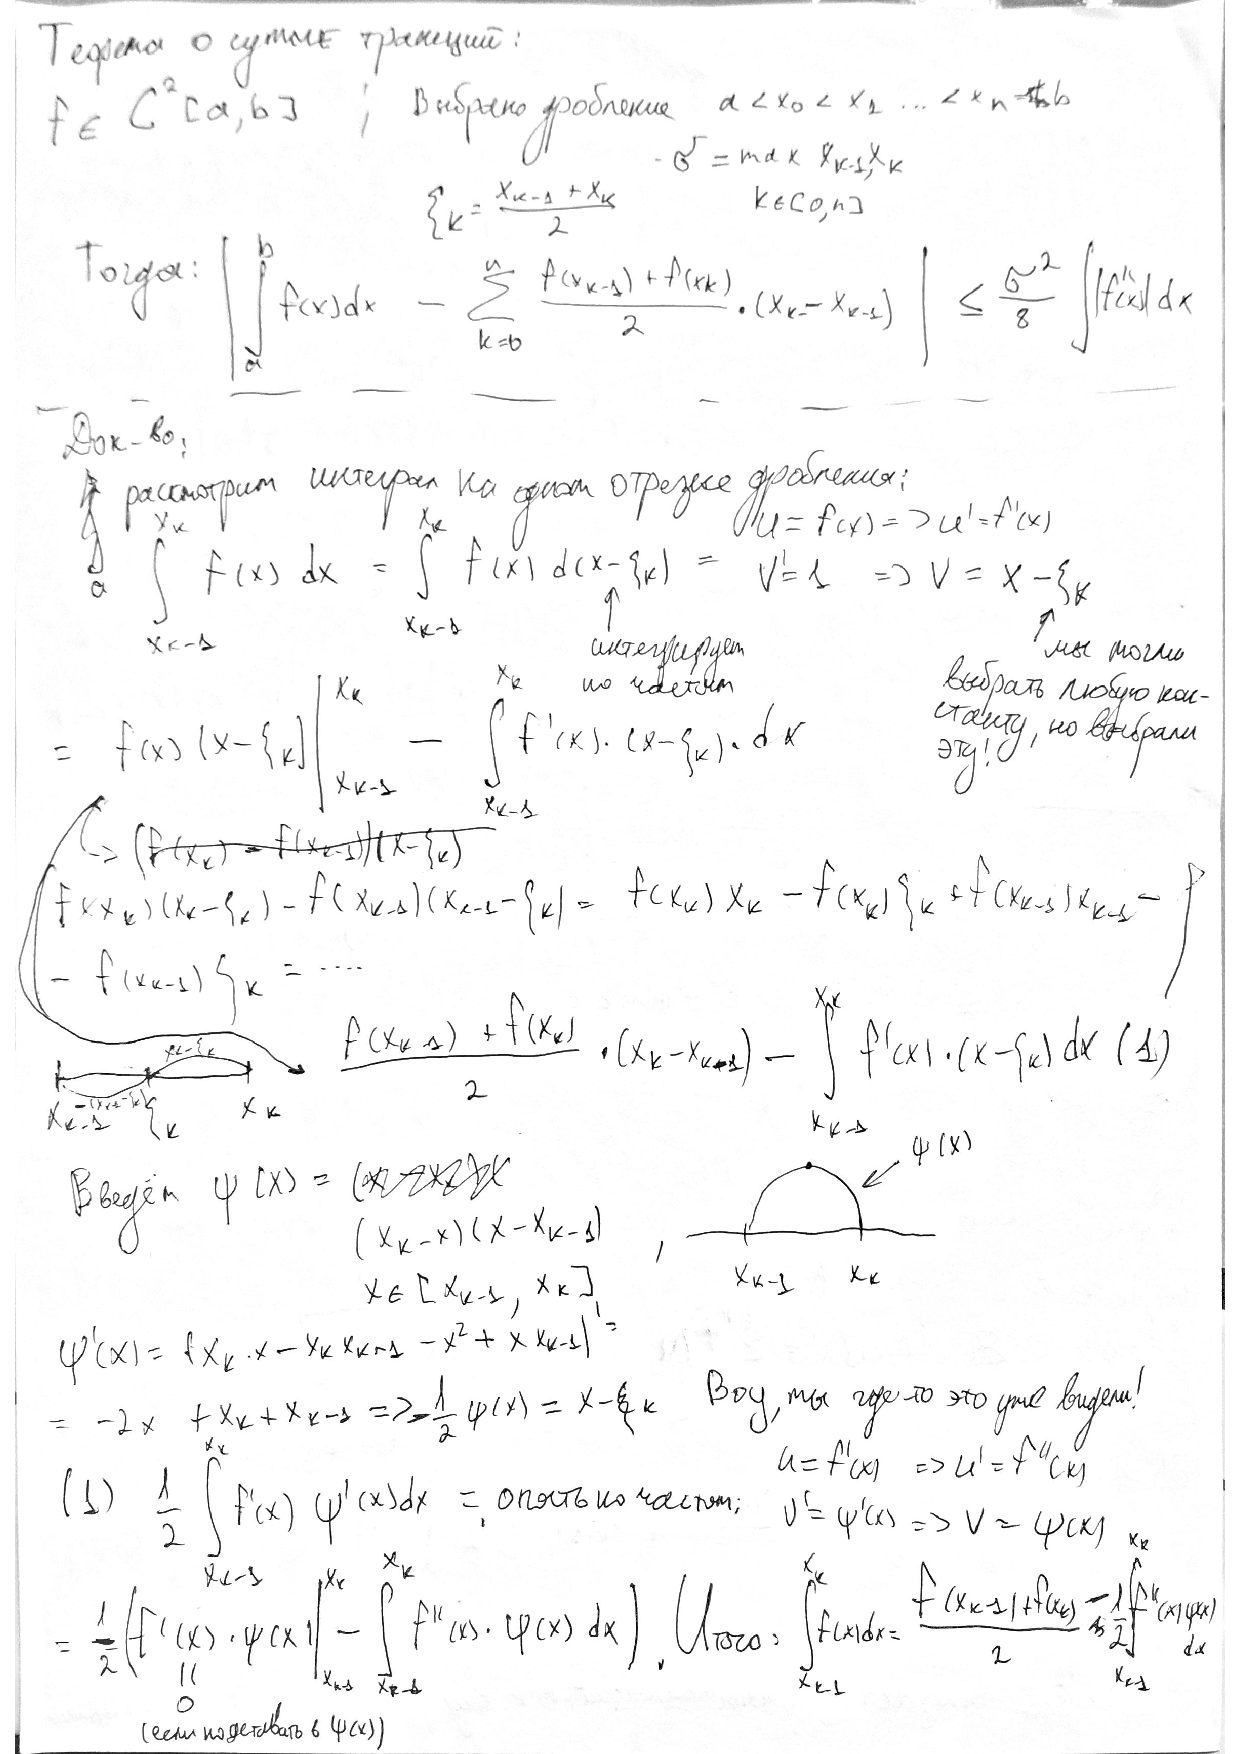
\includepdf[pages={-}]{../images/trapezoid_Euler-McLoren.pdf}

\subparagraph{Формулировка (Формула Эйлера--Маклорена):}

$m, n \in \mathbb{Z}, f \in C^2[m, n]$

Тогда 

\[\int_m^nf = \sum_{i = m}^n{f(i)} - \frac{1}{2}\int_m^n{f^{\prime\prime}(x)\{x\}(1 - \{x\})}\]

Причём первое и последнее слагаемое в сумме входят с множителем $\frac{1}{2}$

\subparagraph{Доказательство (Формула Эйлера--Маклорена):}

Выше

\subsubsection{Асимптотика степенных сумм\texorpdfstring{$^2$}{}}
\subparagraph{Формулировка:}

Наша функция $p > 1, f(x) = x^p$. Возьмём сумму первых $n$ членов:
\[1^p + 2^p + \ldots + n^p = \int_1^n{f(x)} = \sum_{i = 1}^{n - 1}{x^p} + \frac{1}{2}1^p + \frac{1}{2}n^p - \frac{1}{2}\int_m^n{p(p - 1)x^{p - 2}\{x\}(1 - \{x\})} \\= \ldots = \frac{n^{p + 1}}{p + 1} + \frac{1}{2}n^p + O(\max{1, n^{p - 1}})\]

\subparagraph{Доказательство:}

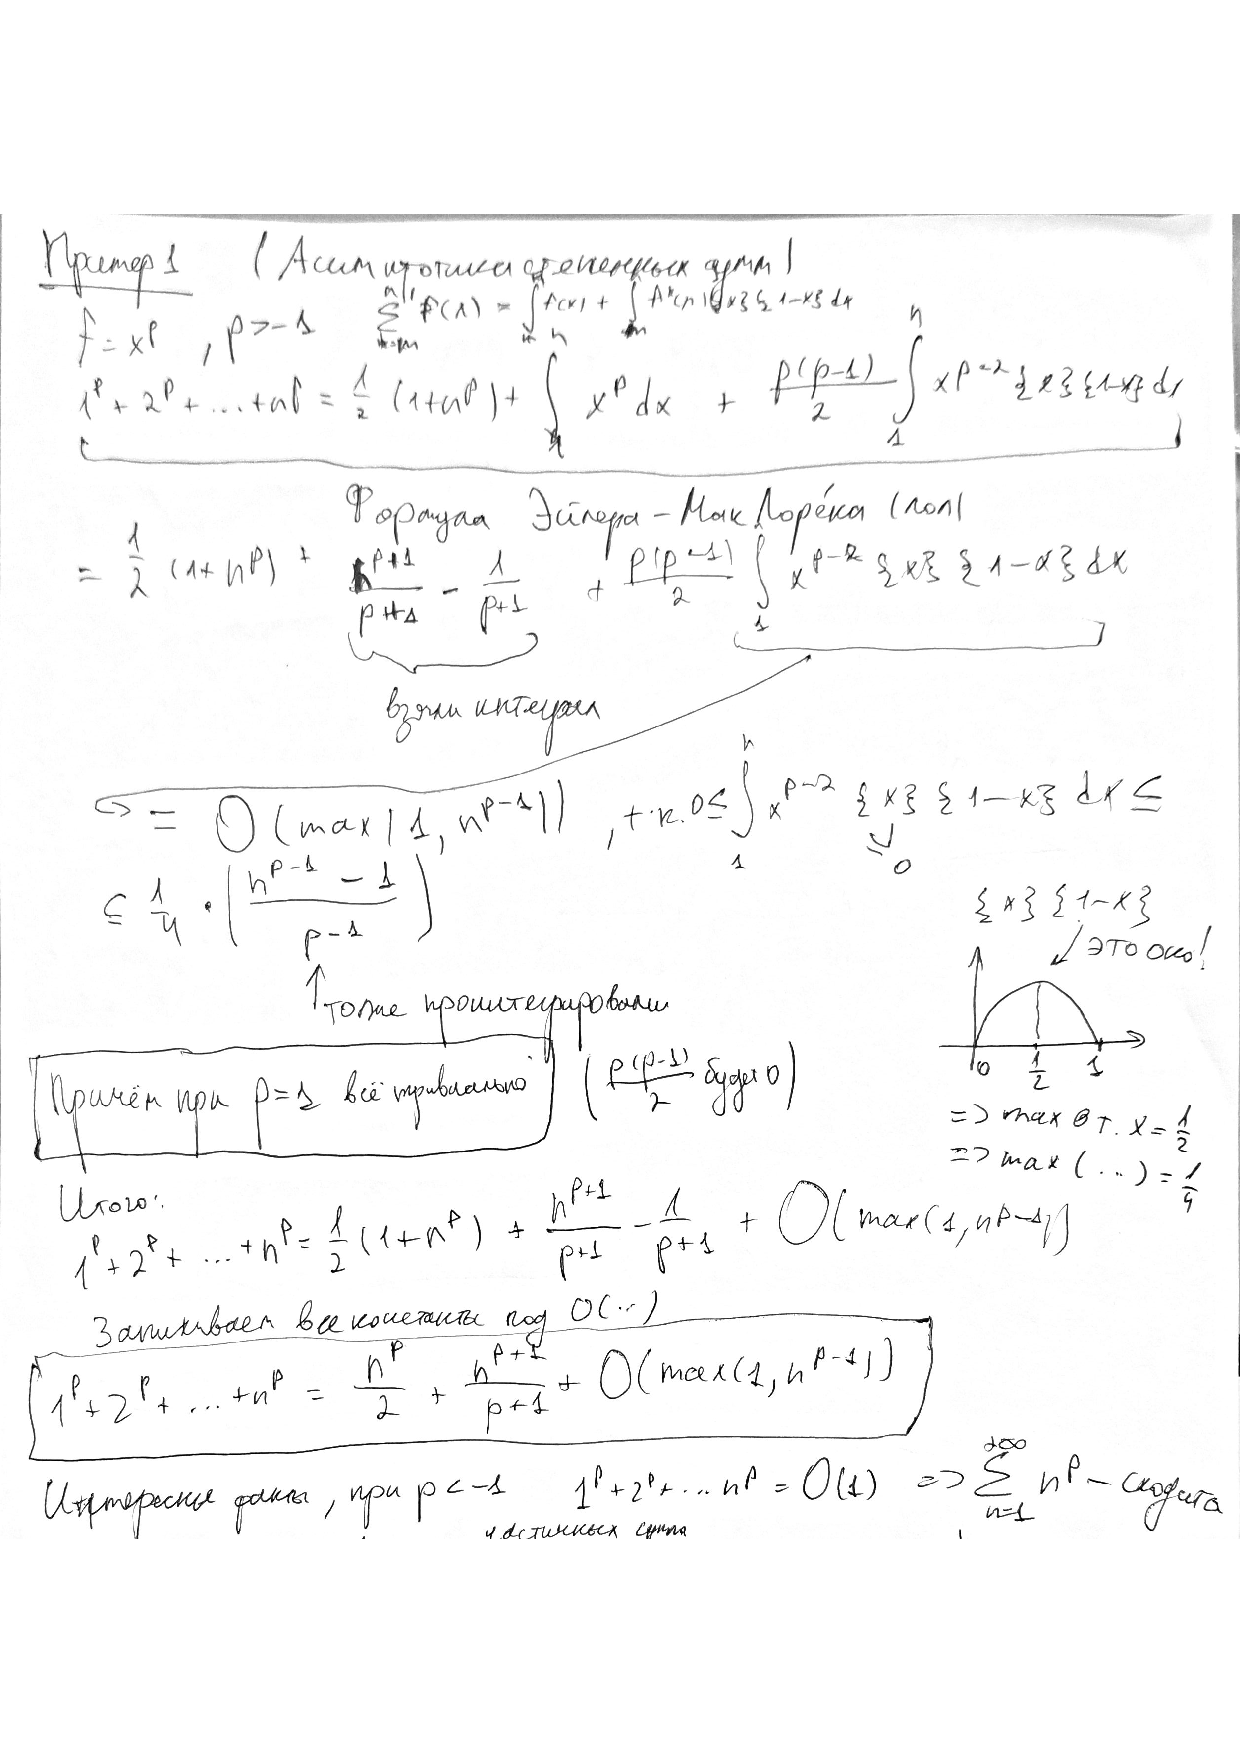
\includepdf[pages={-}]{../images/asym_step.pdf}


\subsubsection{Асимптотика частичных сумм гармонического ряда\texorpdfstring{$^2$}{}}

\subparagraph{Формулировка:}

\[1 + \frac{1}{2} + \frac{1}{3} + \ldots + \frac{1}{n} = \ldots = \ln{n} + \gamma + o(1), \gamma \in \left[\frac{1}{2}, \frac{1}{2} + \frac{1}{8}\right]\]

\subparagraph{Доказательство:}

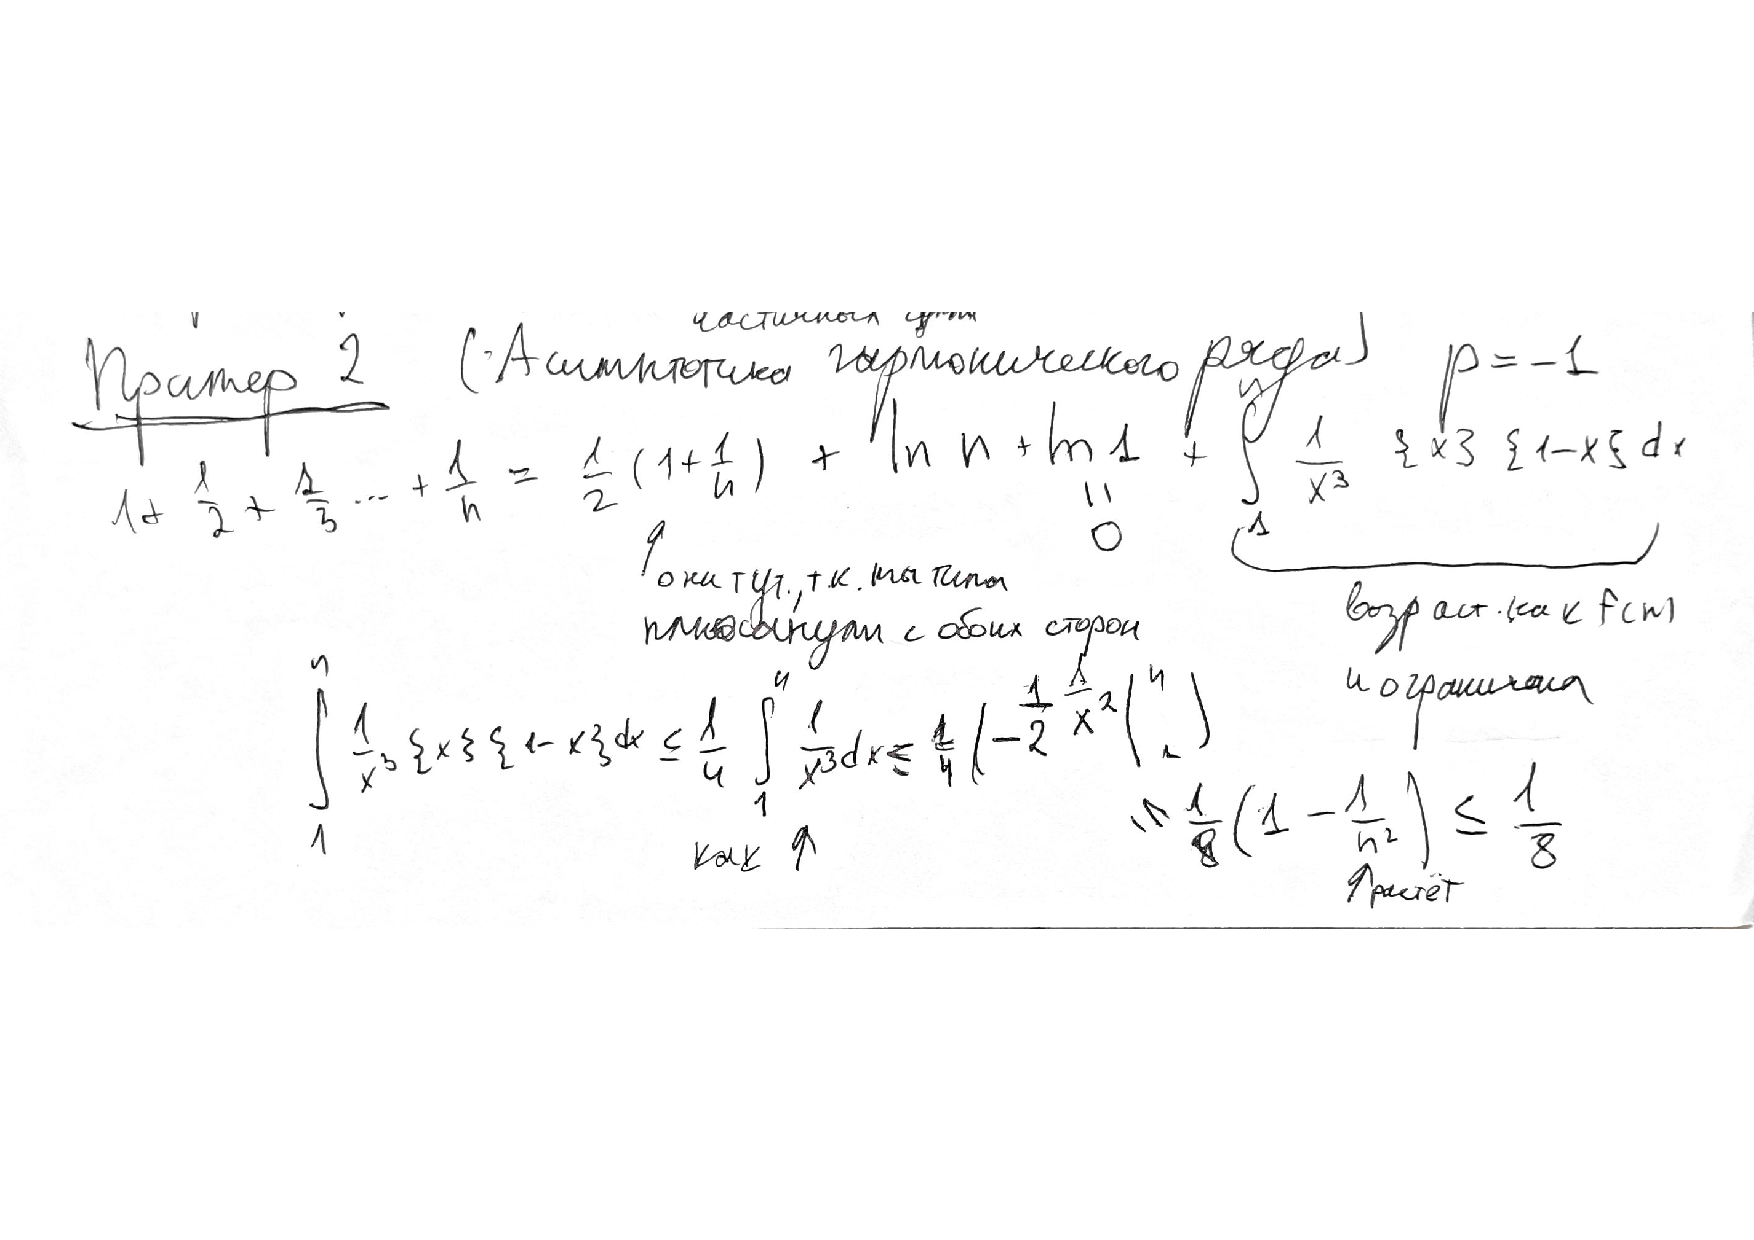
\includepdf[pages={-}, clip, pagecommand={\pagestyle{fancy}}]{../images/asym_garm.pdf}


\subsubsection{Формула Валлиса\texorpdfstring{$^1$}{}}\label{Валлис}
\subparagraph{Формулировка}
$$
\int_0^{\frac{\pi}{2}}\sin^n x \D x = \frac{n-1!!}{n!!}\frac{\pi}{2}, n\text{-- чётно}
$$
$$
\int_0^{\frac{\pi}{2}}\sin^n x \D x = \frac{n-1!!}{n!!}, n\text{-- нечётно}
$$

\subparagraph{Доказательство}
$\rhd$
$$
I_n := \int_0^{\frac{\pi}{2}}\sin^n x \D x
$$

$$
I_0 = \frac{\pi}{2}
$$
$$
I_1 = 1
$$

$$
I_n = \int_0^{\frac{\pi}{2}}\sin^n x \D x = \int_0^{\frac{\pi}{2}}\sin x \cdot \sin^{n-1}x \D x \underset{\text{по частям}}{=} -\cos x \sin^{n-1} x |_0^{\frac{\pi}{2}} + (n-1)\int_0^\frac{\pi}{2} \sin^{n-2}x \cos^2x \D x =
$$

$$
-\cos x \sin^{n-1} x |_0^{\frac{\pi}{2}} = 0
$$

$$
= (n-1)\int_0^\frac{\pi}{2} \sin^{n-2}x (1 - \sin^2x) \D x = (n-1)\int_0^\frac{\pi}{2} (\sin^{n-2}x - \sin^n x) \D x = 
$$
$$
= (n-1)\int_0^\frac{\pi}{2} \sin^{n-2}x \D x - (n-1)\int_0^\frac{\pi}{2} \sin^n x \D x = (n-1) I_{n-2} - (n-1) I_n 
$$
$$
I_n + (n-1)I_n = (n-1)I_{n-2}
$$
$$
I_n = \frac{n-1}{n}I_{n-2}
$$
$\lhd$

\subsubsection{Простейшие свойства несобственного интеграла\texorpdfstring{$^2$}{}}

\subparagraph{Формулировка:}

\begin{enumerate}
    \item \textbf{Критерий Больцано-Коши}
    
    $\lim_{A \rightarrow b - 0}{\int_a^A}$ --- конечный $\Leftrightarrow \forall \varepsilon > 0 \dbl \exists \delta \in (a, b) \dbl \forall A, B \in (\delta, b) \quad \left|\int_A^B\right| < \varepsilon$
    
  \item \textbf{Аддитивность по промежутку}
    
    $f$ --- допустима, $[a, b), c \in (a, b)$. Тогда $\int_a^{\rightarrow b}$ и $\int_c^{\rightarrow b}$ --- сходятся и расходятся одновременно. А если сходятся, то $\int_a^{\rightarrow b} = \int_a^{c} + \int_c^{\rightarrow b}$
    
  \item \textbf{Линейность}
    
    $f, g$ --- допустимы, $\int_a^{\rightarrow b}f, \int_a^{\rightarrow b}g$ --- сходятся, $\lambda \in \mathbb{R}$. Тогда $\lambda f, f \pm g$ --- допустимы, $\int_a^{\rightarrow b}{\lambda f}$ и $\int_a^{\rightarrow b}{f \pm g}$ --- сходятся. 
    
    \begin{enumerate}
        \item $\int_a^{\rightarrow b}{\lambda f} = \lambda \int_a^{\rightarrow b}{f}$
        
         \item $\int_a^{\rightarrow b}{f \pm g} = \int_a^{\rightarrow b}{f} + \int_a^{\rightarrow b}{g}$
    \end{enumerate}
    \item \textbf{Интегрирование неравенств}
    
    $f, g$ --- допустимы, $\int_a^{\rightarrow b}f, \int_a^{\rightarrow b}g$ --- существуют в $\overline{\mathbb{R}}$, $f \le g$ на $[a, b)$. Тогда $\int_a^{\rightarrow b}f \le \int_a^{\rightarrow b}g$
    
    \item \textbf{Интегрирование произведения}
    
    $f, g$ --- дифф. на$[a, b)$, $f^\prime, g^\prime $ --- допустимы. $\Leftrightarrow f, g \in C[a, b]$.
    
    $\int_a^{\rightarrow b}{fg^\prime} = fg|_a^{\rightarrow b} - \int_a^{\rightarrow b}{f^\prime g}$ (если существуют хотя бы 2 предела, то существует и 3й, и равенство выполняется)
    
    \item \textbf{Интегрирование композиции}
    
    $\phi: [\alpha, \beta) \rightarrow \langle A, B \rangle, \phi \in C[\alpha, \beta]$ 
    $f: \langle A, B \rangle \rightarrow \mathbb{R}, \exists \phi(\beta - 0) \in \overline{\mathbb{R}}$
    
    Тогда:
    
    $\int_\alpha^{\rightarrow \beta}{f(\phi(t))\phi^\prime(t)dt} =
     \int_{\phi(\alpha)}^{\rightarrow \phi(\beta - 0)}{f(x)dx}$
     
     \textit{Примечание:}
     $f$ --- кусочно непрерывна на $[a, b]$. Если рассмотреть на $[a, b)$, то $\int_a^{\rightarrow b}{f} = \int_a^b{f}$
    

\end{enumerate}

\subparagraph{Доказательство:}

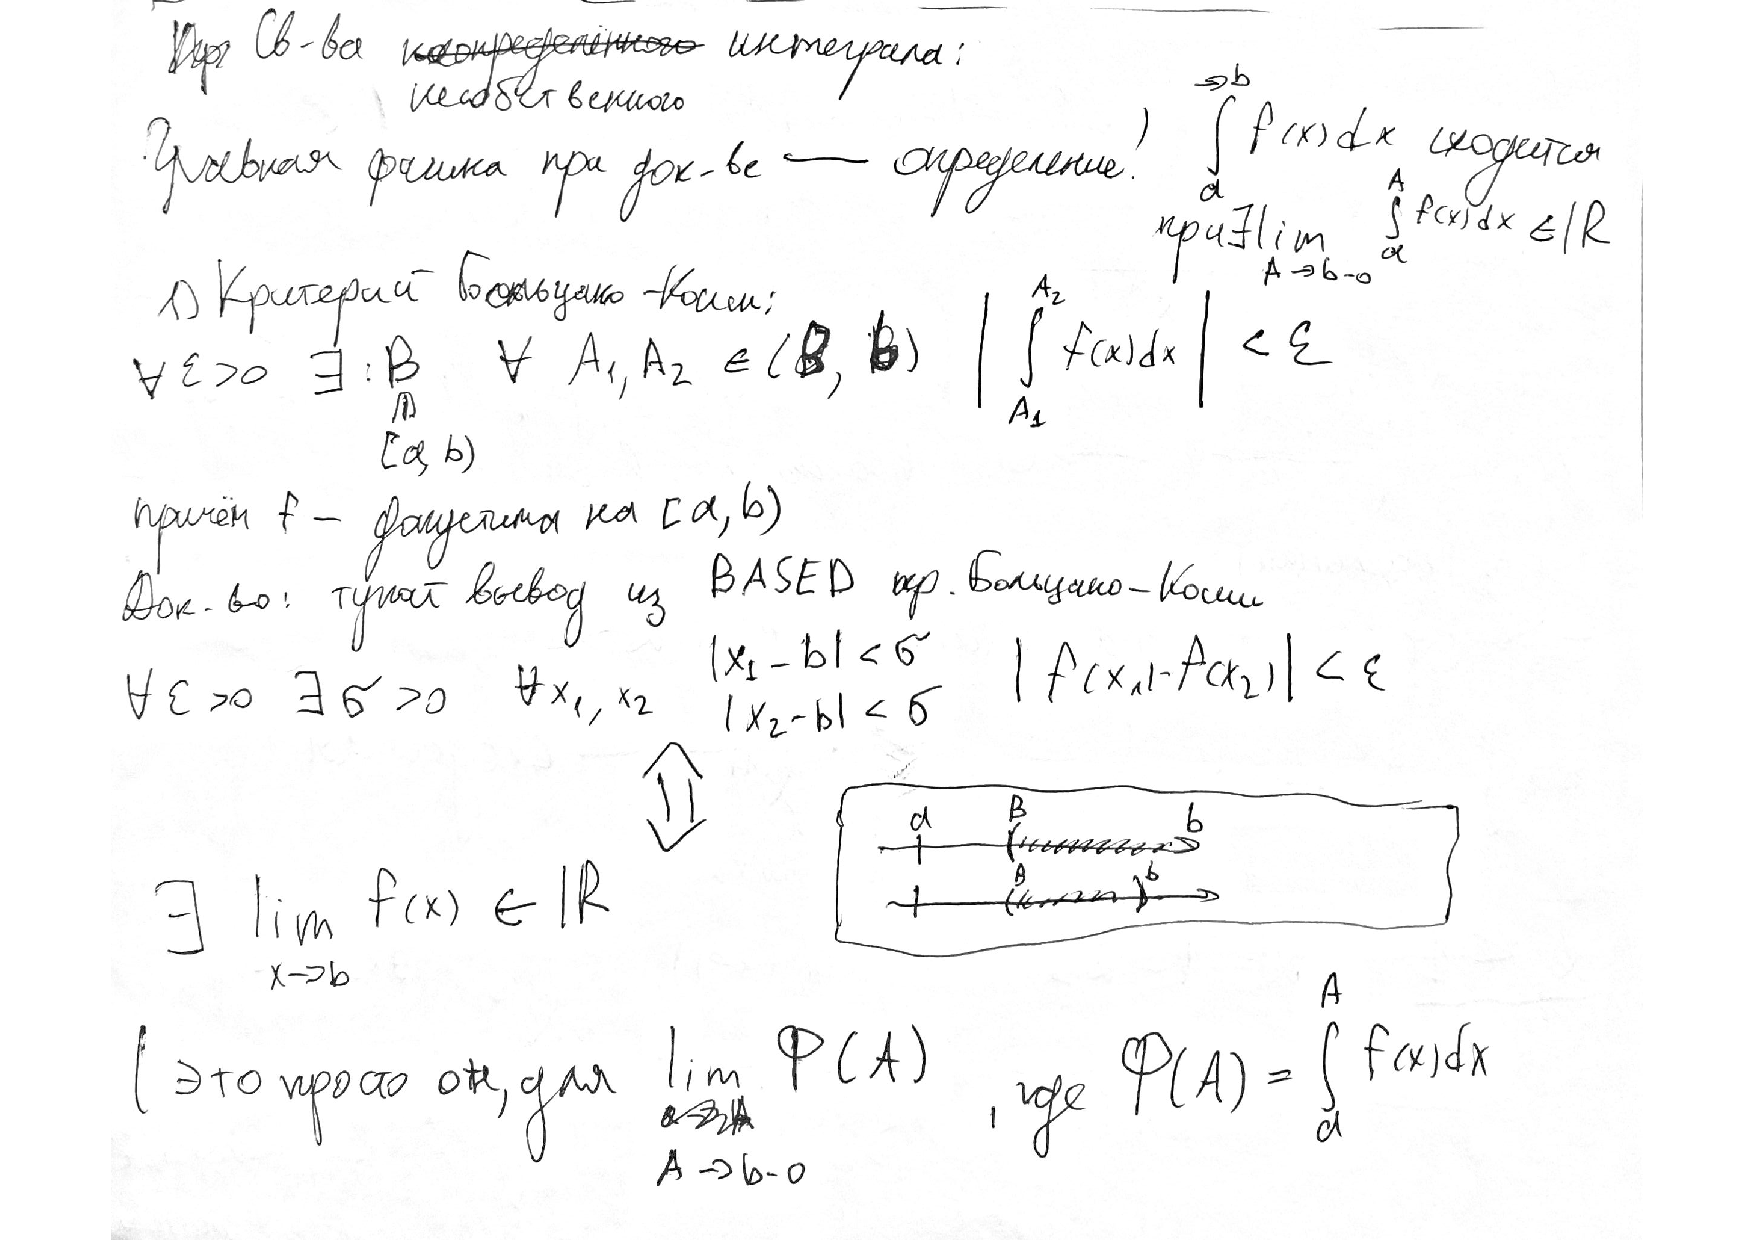
\includepdf[pages={-}]{../images/pr_svva_nes_int.pdf}


\subsubsection{Изучение сходимости интеграла \texorpdfstring{$\int_{10}^\infty \frac{dx}{x^\alpha (\ln x)^\beta}$}{int [10, inf] dx/x\^a(ln x)\^b}\texorpdfstring{$^2$}{}}

\subparagraph{Формулировка:}

$\int_{10}^\infty \frac{dx}{x^\alpha (\ln x)^\beta}$

\subparagraph{Доказательство:}

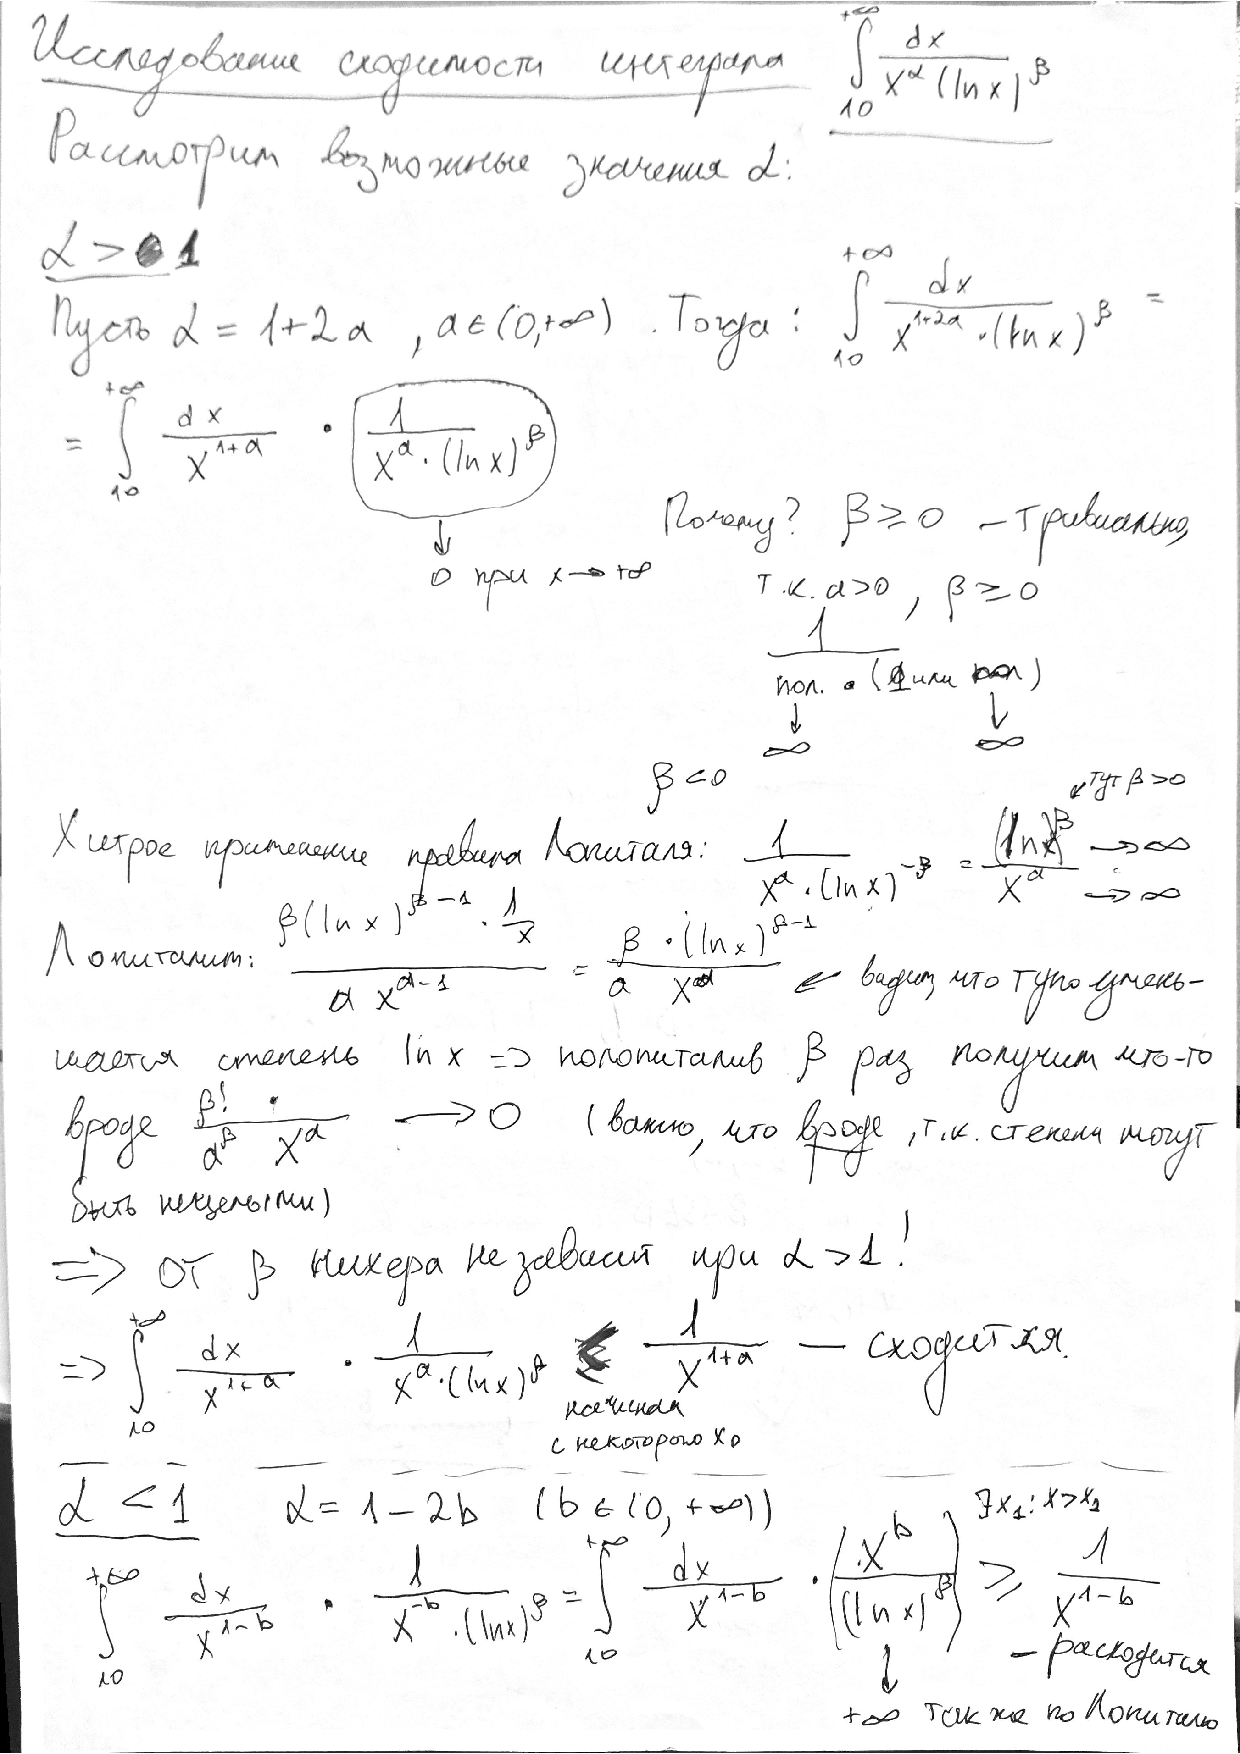
\includepdf[pages={-}]{../images/issl_sh_iks_log.pdf}

\section{Период Мезозойский}
\subsection{Важные определения}
\subsubsection{Гамма функция Эйлера\texorpdfstring{$^1$}{}}
$$
\Gamma(x) = \int^{+\infty}_0 t^{x-1} e^{-t} \D t
$$

\subsubsection{Абсолютно сходящийся интеграл, ряд\texorpdfstring{$^1$}{}}
\paragraph{Интеграл}
$\letus f: [ a, b ) \rightarrow \mathbb{R} $ допустима

Несобственный интеграл называется абсолютно сходящимся, когда выполняются 2 условия:
\begin{enumerate}
    \item $\int_a^{\rightarrow b} f(x) \D x$ сходится
    \item $\int_a^{\rightarrow b} |f(x)| \D x$ сходится
\end{enumerate}

\paragraph{Ряд}
$\letus a_n$
\begin{enumerate}
    \item $\sum_{n=1}^{+\infty} a_n$ сходится
    \item $\sum_{n=1}^{+\infty} |a_n|$ сходится
\end{enumerate}

\subsubsection{Числовой ряд, сумма ряда, сходимость, расходимость\texorpdfstring{$^1$}{}}
\paragraph{Числовой ряд}
Выражение
$$
\sum_{k=1}^{+\infty} a_k \quad | \quad a_1+a_2+a_3+\ldots
$$
называется формальным рядом. Введём понятие частичных сумм:
$$
S_N = a_1+a_2+\ldots+a_N
$$
Тогда ряд можно представить как предел последовательности частичных сумм:
$$
\lim_{N\rightarrow +\infty} S_N = S
$$

\paragraph{Сумма ряда}
$S$ называют суммой ряда.
\paragraph{Сходимость}
Если $S \in \mathbb{R}$, то такой ряд называют сходящимся
\paragraph{Расходимость}
Если $S = \pm\infty$ или $\nexists \lim S_N$, то такой ряд называют расходящимся



\newpage
\subsection{Определения}

\subsubsection{\texorpdfstring{$n$}{n}-й остаток ряда\texorpdfstring{$^1$}{}}
$R_N = \sum_{k=N}^{+\infty} a_k$ --- $N$-ый остаток ряда.

\subsubsection{Критерий Больцано--Коши сходимости числового ряда\texorpdfstring{$^1$}{}}
\nameref{КБК}

\newpage
\subsection{Важные теоремы}
\subsubsection{Гамма функция Эйлера. Простейшие свойства.\texorpdfstring{$^1$}{}}
\subparagraph{Формулировка + доказательство}
\begin{enumerate}
    \item Область определения
    
    Поищем где интеграл сходится:
    
    Рассмотрим промежуток интегрирования от 0 до 1. Очевидно, при $t\rightarrow 0 \quad t^{x-1} e^{-t} \equiv t^{x-1}$. Ну а так как $x-1 > -1$, то и интеграл сходится. Обратите внимание, это именно то условие, почему при $x \le 0$ всё ломается.
    
    Теперь осталось посмотреть на промежуток от 1 до $+\infty$:
    Надо просто заметить что экспонента стремится к нулю быстрее, чем возрастает $t^{x-1}$. Соответственно, мы можем отломить от неё кусок, заметив, что вся наша формула неотрицательна (т.к. все члены положительны):
    $$
    0 \le t^{x-1} e^{-t} = t^{x-1} e^{-\frac t2} e^{-\frac t2}
    $$
    Так как экспонента стремится к нулю быстрее при росте $t$, а $t^{x-1}$ ограничена, то $t^{x-1} e^{-\frac t2}$ тоже стремится к нулю, а значит:
    $$
    t^{x-1} e^{-\frac t2} e^{-\frac t2} \le e^{-\frac t2}
    $$
    А это уже стремится к нулю, то есть интеграл сходится.
    
    
    \item Выпуклость
    
    Зафиксируем $t$ и рассмотрим подынтегральную функцию. Тогда формула превратится в $f(x) = t^{x-1}e^{-t}$. Теперь мы смотрим на $t$ как на константу и видим произведение показательной функции с какой-то константой. Показательная функция выпукла $\implies f(\alpha_1 x_1 + \alpha_2 x_2) \le \alpha_1 f(x_1) + \alpha_2 f(x_2)$. Теперь если всё это безобразие проинтегрировать и подшаманить, то получится $$
    \int^{+\infty}_0 t^{\alpha_1 x_1 + \alpha_2 x_2 -1} e^{-t} \D t \le \alpha_1 \int^{+\infty}_0 t^{x_1-1} e^{-t} \D t + \alpha_2 \int^{+\infty}_0 t^{x_2-1} e^{-t} \D t
    $$
    
    А это определение выпуклости нашей рассматриваемой функции. BTW, из выпуклости следует непрерывность этой функции на всей области определения.
    
    \item Значение
    Проинтегрируем нашу гамма-функцию по частям:
    $$
    \Gamma(x+1) = \int^{+\infty}_0 t^{x} e^{-t} \D t = -t^x e^{-t} |^{+\infty}_0 + x\int^{+\infty}_0 t^{x-1} e^{-t} \D t = 0 + x\int^{+\infty}_0 t^{x-1} e^{-t} \D t = x\cdot \Gamma(x)
    $$
    
    Теперь заметим, что $\Gamma(1) = 1$, из чего по индукции получаем $\Gamma(n+1) = n!$
    
    \item График
    
    Рассмотрим $\Gamma(x) = \frac{\Gamma(x+1)}{x}$
    
    При $x \rightarrow 0 \quad \Gamma(x+1) \rightarrow \Gamma(1) = 1 \Rightarrow \Gamma(x) = \frac{\Gamma(x+1)}{x} \rightarrow \frac 1x$ 
    
    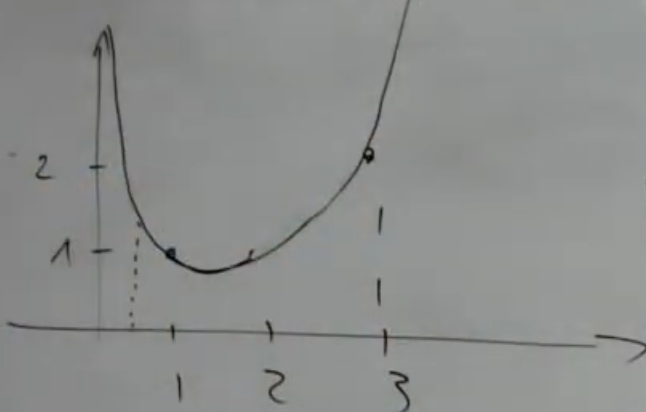
\includegraphics[]{../images/gamma-euler.png}
    
    \item Связь с $\pi$
    $$
    \Gamma(\frac 12) = \int_0^{+\infty} t^{-\frac 12} e^{-t} \D t \underset{t:= x^2}{=} 2\int_0^{+\infty} x \cdot x^{-1} e^{-x^2} \D x = 2\int_0^{+\infty} e^{-x^2} \D x \underset{\text{\nameref{ИЭП}}}{=} \sqrt \pi
    $$
\end{enumerate}


\subsubsection{Неравенство Йенсена для сумм\texorpdfstring{$^1$}{}}
\subparagraph{Формулировка}
$f: \langle a, b \rangle \rightarrow \mathbb{R}$ выпуклая.

$\forall x_1, x_2, \ldots, x_n \in [a, b]$

$\forall \alpha_1, \alpha_2, \ldots, \alpha_n : \sum_i \alpha_i = 1$

$$
f(\alpha_1 x_1 + \alpha_2 x_2 + \ldots + \alpha_n x_n) \le \alpha_1 f(x_1) + \alpha_2 f(x_2) + \ldots + \alpha_n f(x_n)
$$


\subparagraph{Доказательство}

Пользуясь выпуклостью, мы можем провести опорную прямую такую, что $f(x)$ будет выше этой прямой. Нас интересует прямая в точке $x^* := \alpha_1 x_1 + \alpha_2 x_2 + \ldots + \alpha_n x_n$ по условию. Но сначала надо убедиться, что точка лежит в $\langle a, b \rangle$:
$$
a \le \min_{i}(x_i) \le \sum_i \alpha_i \cdot x_i \le \sum_i \alpha_i \cdot \max_j (x_j) = \max_j (x_j) \sum_i \alpha_i = \max_j (x_j) \le b
$$

Теперь проводим опорную прямую:
$$
f(x^*) = kx^* + b = \sum_i(k \alpha_i \cdot x_i) + b = \sum_i(k \alpha_i \cdot x_i + b\cdot\alpha_i) = \sum_i(\alpha_i (k \cdot x_i + b)) \le \sum_i\alpha_i f(x_i) 
$$
Note: $b = \sum_i(\alpha_i \cdot b)$, так как сумма $\alpha_i = 1$


\subsubsection{Неравенство Гельдера для интегралов\texorpdfstring{$^2$}{}}
\textit{Формулировка}

Пусть $f, g \in C[a, b]; \frac{1} {p} + \frac{1} {q} = 1$. Тогда
\begin{equation*}
\left|\int_a^b fg\right| \leq \left(\int_a^b |f|^p\right)^{1/p} \left(\int_a^b |g|^q\right)^{1/q}
\end{equation*}
\begin{proof}
Распишем интегральные суммы: $x_k := a + k\frac{b - a} {n}; \Delta x_k = \frac{b - a} {n}$. Пусть $a_i = f(x_k) (\Delta x_k)^{1/p}, b_i = g(x_k) (\Delta x_k)^{1/q}$, тогда, по неравенству Гёльдера для сумм:
\begin{align*}
\left|\sum f(x_k) g(x_k) (\Delta x_k)^{\frac{1} {p} + \frac{1} {q}} \right| &\leq \left(\sum|f(x_k)|^p \Delta x_k\right)^{1/p} \left(\sum|g(x_k)|^q \Delta x_k\right)^{1/q}\\
\left|\sum f(x_k) g(x_k)  \right| &\leq \left(\sum|f(x_k)|^p \right)^{1/p} \left(\sum|g(x_k)|^q \right)^{1/q}
\end{align*} 
Осталось лишь сделать предельный переход при $n \to \infty$
\begin{equation*}
\left|\int_a^b fg\right| \leq \left(\int_a^b |f|^p\right)^{1/p} \left(\int_a^b |g|^q\right)^{1/q}
\end{equation*}
\end{proof}

\subsubsection{Признак сравнения сходимости положительных рядов\texorpdfstring{$^1$}{}}
\paragraph{Лемма о сходимости положительных рядов}
\subparagraph{Формулировка}
$a_n \ge 0$

$\sum a_n$ сходится $\Leftrightarrow S_n$ ограничено.
\subparagraph{Доказательство}
Тривиально следует из того, что ввиду того, что $a_n \ge 0$, последовательность частичных сумм $S_n$ монотонно возрастает. То есть оно ограничено своим пределом частичных сумм и монотонно к нему стремится снизу.

\paragraph{Теорема}
\subparagraph{Формулировка}
$\letus a_n \ge 0, b_n \ge 0, \sum a_n, \sum b_n$
\begin{enumerate}
    \item $a_n \le b_n \Rightarrow \sum b_n$ сходится $\Rightarrow \sum a_n$ сходится, $\sum a_n$ расходится $\Rightarrow \sum b_n$ расходится. 
    
    Замечание: аналогичное утверждение верно для $\forall k a_n \le k \cdot b_n$, так как сходимость $b_n$ и $k \cdot b_n$ эквивалентна и можно безопасно их тут подменить.
    
    \item $\exists \lim \frac{a_n}{b_n} = l$. Тогда 
    если $l \in \mathbb{R}_+$, то сходимость $\sum a_n$ эквивалентна сходимости $\sum b_n$.

    Если $l = \infty$, то $\sum a_n$ сходится $\Rightarrow \sum b_n$ сходится, $\sum b_n$ расходится $\Rightarrow \sum a_n$ расходится.
    
    Если $l = 0$, то $\sum b_n$ сходится $\Rightarrow \sum a_n$ сходится, $\sum a_n$ расходится $\Rightarrow \sum b_n$ расходится.
\end{enumerate}

\subparagraph{Доказательство}
\begin{enumerate}
    \item Воспользуемся приведённой леммой и просто сведём наши сходящиеся ряды к частичным суммам и обратно:
    $a_n \le b_n \Rightarrow S_n^{(a)} \le S_n^{(b)}$. Положим $\sum b_n$ сходится, тогда по лемме $S_n^{(b)}$ ограничено. Тогда $S_n^{(a)}$ тоже ограничено, а значит и $\sum a_n$ сходится. Аналогично работает наоборот.
    
    \item Давайте всё сведём к предыдущему пункту. Если $l \in \mathbb{R}_+$, то мы всегда можем домножить $a_n$ на какое-то вещественное число, чтобы оно стало меньше $b_n$ (т.к. начиная с какого-то $n$ частное всей последовательности будет лежать в какой-то окрестности $l$). Также наоборот, мы всегда можем сделать $k \cdot a_n > b_n$, то есть мы получили первое утверждение в обоих случаях симметрично. То есть действительно сходимость у этих рядов эквивалентна. 
    
    Примечание: то, что мы рассматриваем сходимость рядов начиная с какого-то $n$, абсолютно законно, так как мы ранее доказывали эквивалентность сходимости $n$--го остатка и самого ряда.
    
    При $l = \infty$ всё тривиально, так как в этом случае начиная с какого-то места, очевидно, $a_n > b_n$, что уже свелось к первому признаку. Для $l = 0$ аналогично.
\end{enumerate}

\paragraph{Важные эталонные ряды, с которыми надо всё сравнивать}
\begin{enumerate}
    \item $\sum \frac{1}{n^p}$ расходится при $p \le 1$, сходится при $p > 1$.
    \item $\sum q^n$ сходится при $0 < q < 1$, расходится при $q \ge 1$.
\end{enumerate}

\subsubsection{Признак Коши сходимости положительных рядов\texorpdfstring{$^1$}{}}
\label{КошиРяды}
\subparagraph{Формулировка}
$$
\sum a_n \ge 0; \letus k_n = \sqrt[n]{a_n}
$$
Тогда:
\begin{enumerate}
    \item Начиная с какого-то места $\exists q : k_n < q < 1$ ($q$ мы ввели чтобы потом сравнивать с ним, так как признак сравнения у нас строго $<1$ и с $1$ сравнивать неудобно) $\Rightarrow \sum a_n$ сходится
    \item $\exists$ бесконечное число элементов $k_n \ge 1 \Rightarrow \sum a_n$ расходится.
\end{enumerate}

\subparagraph{Доказательство}
\begin{enumerate}
    \item Выразим из "волшебного" $k_n$ нормальный $a_n$. $k_n = \sqrt[n]{a_n} \Rightarrow a_n = k_n^n < q^n$. У нас $q < 1$, а значит можно сравнить его с ближайшим рациональным $<1$ и у нас получается эталонный $\frac{1}{\alpha^n}$ где $n$ у нас, разумеется $> 1$, а значит всё сходится.
    \item Прошлая стратегия не работает т.к. $q \ge 1$, а значит мы не подберём рациональную дробь для эталонного. Но зато у нас тут не выполнится необходимый признак сходимости, так как $k_n$ не стремится к 0, сколько не возводи его в большую степень, он только увеличится.
\end{enumerate}

\newpage
\subsection{Теоремы}
\subsubsection{Интеграл Эйлера--Пуассона\texorpdfstring{$^1$}{}}\label{ИЭП}
\subparagraph{Формулировка}
$$
\int_0^{+\infty}e^{-x^2}\D x = \frac{\sqrt{\pi}}{2}
$$

\subparagraph{Доказательство}
Простое неравенство, которое непросто запомнить:
$$
1 - x^2 \le e^{-x^2}\le \frac{1}{1 + x^2}
$$
Следует из выпуклости ($e^t \ge 1 + t$) и работает для $x \in \mathbb{R}$

Как обычно, проинтегрируем (неравенство по середине выражения обуславливается положительностью функции) и возведём всё в степень $n$:
$$
\int_0^1 (1-x^2)^n\D x \le \int_0^1 e^{-nx^2}\D x \le \int_0^{+\infty} e^{-nx^2}\D x \le \int_0^{+\infty} \frac{1}{(1+x^2)^n} \D x 
$$

Теперь аккуратно считаем части неравенства:
$$
\int_0^1 (1-x^2)^n\D x \underset{x := \cos t}{=} \int_0^{\frac \pi 2}(\sin t)^{2n+1}\D t = \underset{\text{\nameref{Валлис}}}{=} \frac{(2n)!!}{(2n+1)!!}
$$

$$
\int_0^1 e^{-nx^2}\D x \underset{t:= \sqrt n \cdot x}{=} \frac{1}{\sqrt n} \int_0^{+\infty}e^{-t^2}\D t
$$

$$
\int_0^{+\infty} \frac{1}{(1+x^2)^n} \D x \underset{x:= \tg t}{=} \int_0^{\frac \pi 2} \cos^{2n-2}{t} \D t \underset{\text{\nameref{Валлис}}}{=} \frac{(2n-3)!!}{(2n-2)!!} \frac \pi 2
$$

Домножаем наши достижения на $\sqrt n$:
$$
\frac{(2n)!! \sqrt{n}}{(2n+1)!!} \le \int_0^{+\infty}e^{-t^2}\D t \le \frac{(2n-3)!!}{(2n-2)!!} \frac \pi 2 \sqrt n
$$

Предельный переход:
$$
\frac{(2n)!!}{(2n-1)!!}\cdot \frac{1}{\sqrt n} \underset{\text{\nameref{Валлис}}}{\longrightarrow} \sqrt \pi
$$

$$
\frac{\sqrt n}{2n + 1} \equiv \frac 1 {2\sqrt n}
$$

$$
\frac{(2n)!! \sqrt{n}}{(2n+1)!!} = \frac{(2n)!!}{(2n-1)!!} \frac{\sqrt n}{2n+1} \equiv \frac{(2n)!!}{(2n-1)!!} \frac{1}{\sqrt n} \frac 1 2 \underset{\text{\nameref{Валлис}}}{\longrightarrow} \frac{\sqrt \pi}{2}
$$

$$
\frac{(2n-3)!!}{(2n-2)!!} \frac \pi 2 \sqrt n = \frac{1}{\frac{(2n-2)!!}{(2n-3)!!}\cdot\frac{1}{\sqrt{n-1}}} \cdot \frac{\sqrt{n}}{\sqrt{n-1}} \cdot \frac \pi 2 \rightarrow \frac{1}{\sqrt\pi} \cdot 1 \cdot \frac \pi 2 = \frac{\sqrt \pi}{2}
$$

По Т. О двух городовых 
$$
\int_0^{+\infty}e^{-t^2}\D t = \frac{\sqrt \pi}{2}
$$


\subsubsection{Теорема об абсолютно сходящихся интегралах и рядах\texorpdfstring{$^1$}{}}
\subparagraph{Формулировка}
\paragraph{Интегралы}
$\letus f: [a, b) \rightarrow \mathbb{R}$ допустима

Тогда эквивалентны следующие утверждения:
\begin{enumerate}
    \item $\int_a^b f(x) \D x$ абсолютно сходится
    \item $\int_a^b |f(x)| \D x$ сходится
    \item $\int_a^b f_+$ и $\int_a^b f_-$ сходятся
\end{enumerate}

\paragraph{Ряды}
$\letus a_n$ ряд.

Тогда эквивалентны следующие утверждения:
\begin{enumerate}
    \item $\sum_{n=1}^{+\infty} a_n$ абсолютно сходится
    \item $\sum_{n=1}^{+\infty} |a_n|$ сходится
    \item $\sum_{n=1}^{+\infty} a_n^+$ и $\sum_{n=1}^{+\infty} a_n^-$ сходятся
\end{enumerate}

\subparagraph{Доказательство}
\underline{$1 \rightarrow 2$}

По определению абсолютной сходимости

\underline{$2 \rightarrow 3$}

Заметим, что $f_+$ и $f_-$ либо положительны, либо константный $0$. Другими словами, одна из срезок будет равна $|f(x)|$, а другая в это время будет равна $0$. Соответственно, существует конечный предел $f(x)$ при $x \rightarrow b-0$. Ну а значит, что и срезка будет его иметь и всё сойдётся. В $0$ проблем не будет по Т. О стабилизации знака.

\underline{$3 \rightarrow 1$}

Очевидно, т.к. можно выразить $f = f_+ - f_-$

\subsubsection{Изучение интеграла \texorpdfstring{$\int_1^{\infty} \frac{\sin x\,dx}{x^p}$}{int [1, inf] sin(x) dx / x\^p} на сходимость и абсолютную сходимость\texorpdfstring{$^2$}{}}

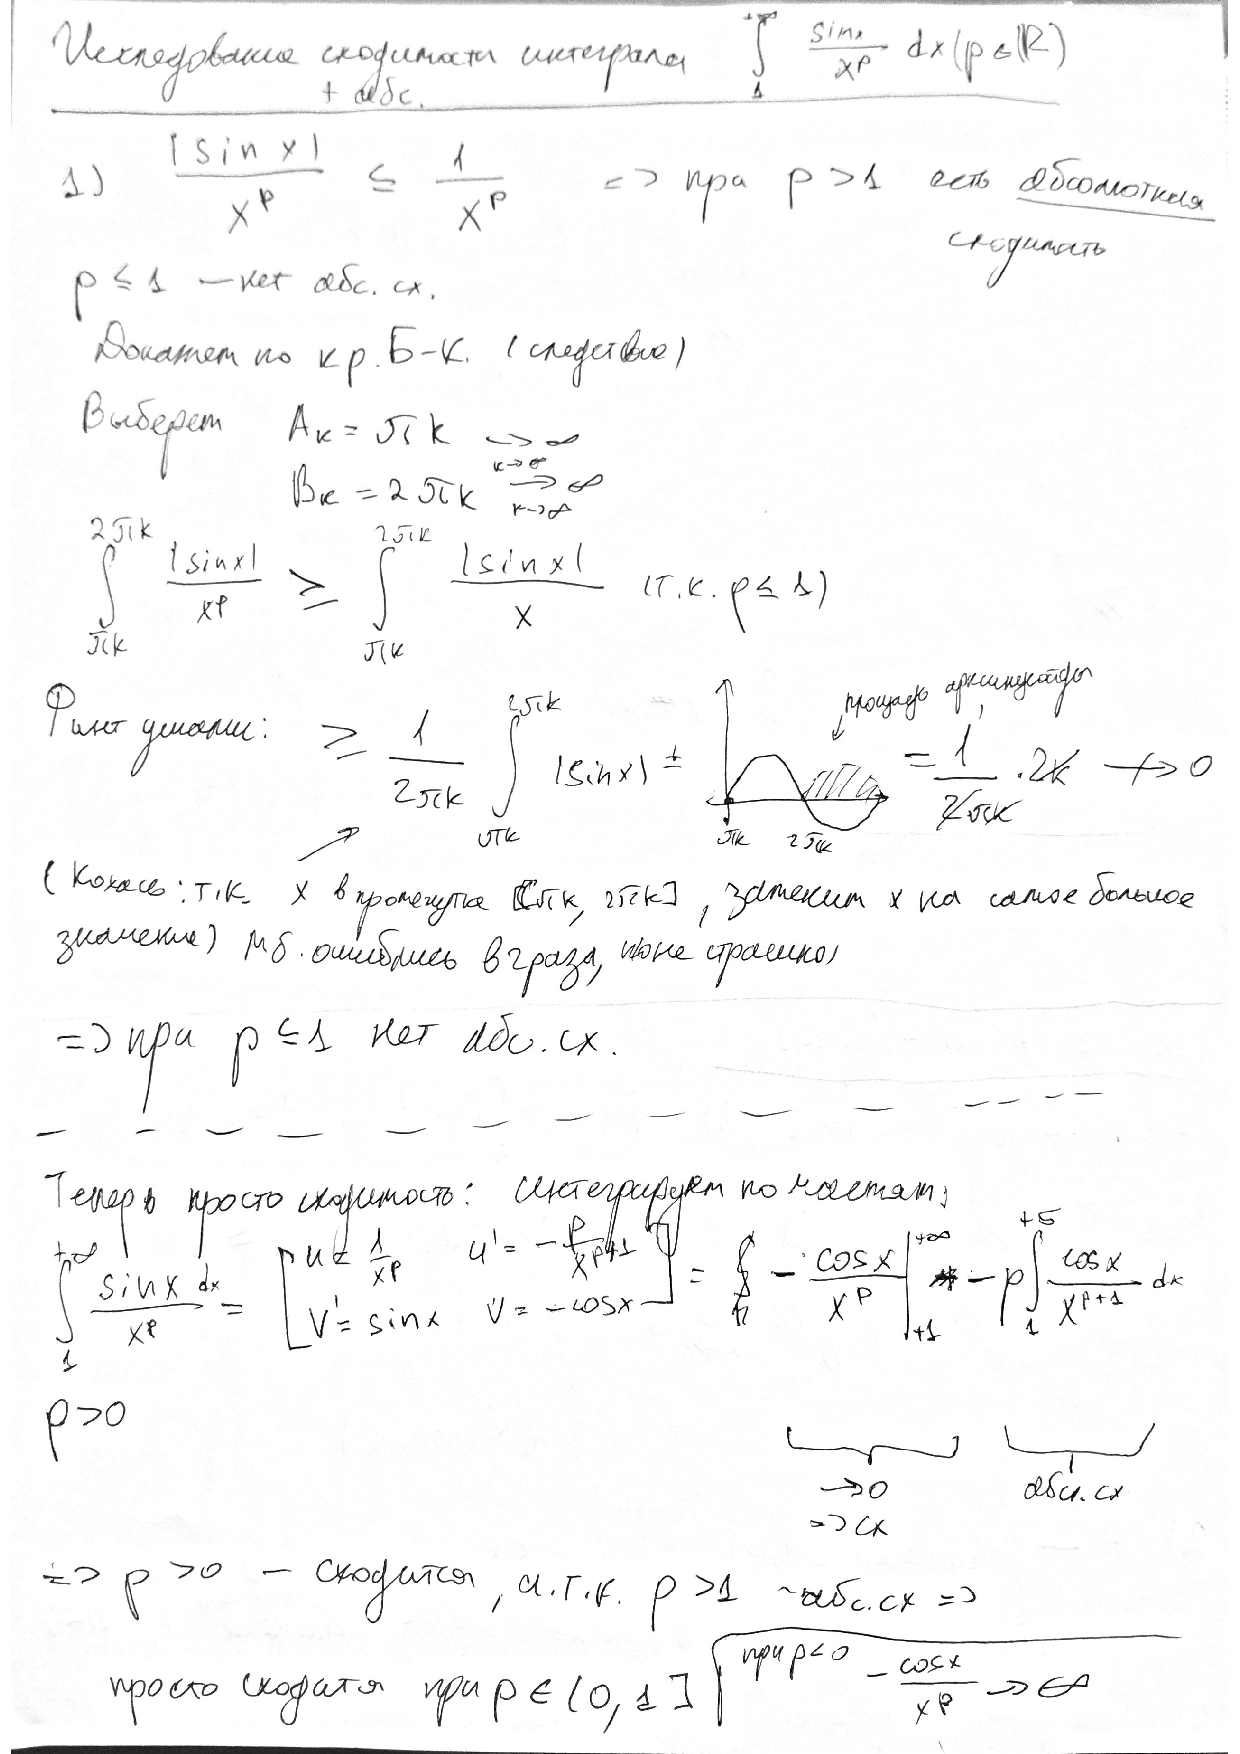
\includepdf[pages={-}]{../images/cov_sinx.pdf}

\subsubsection{Признак Абеля--Дирихле сходимости несобственного интеграла\texorpdfstring{$^2$}{}}

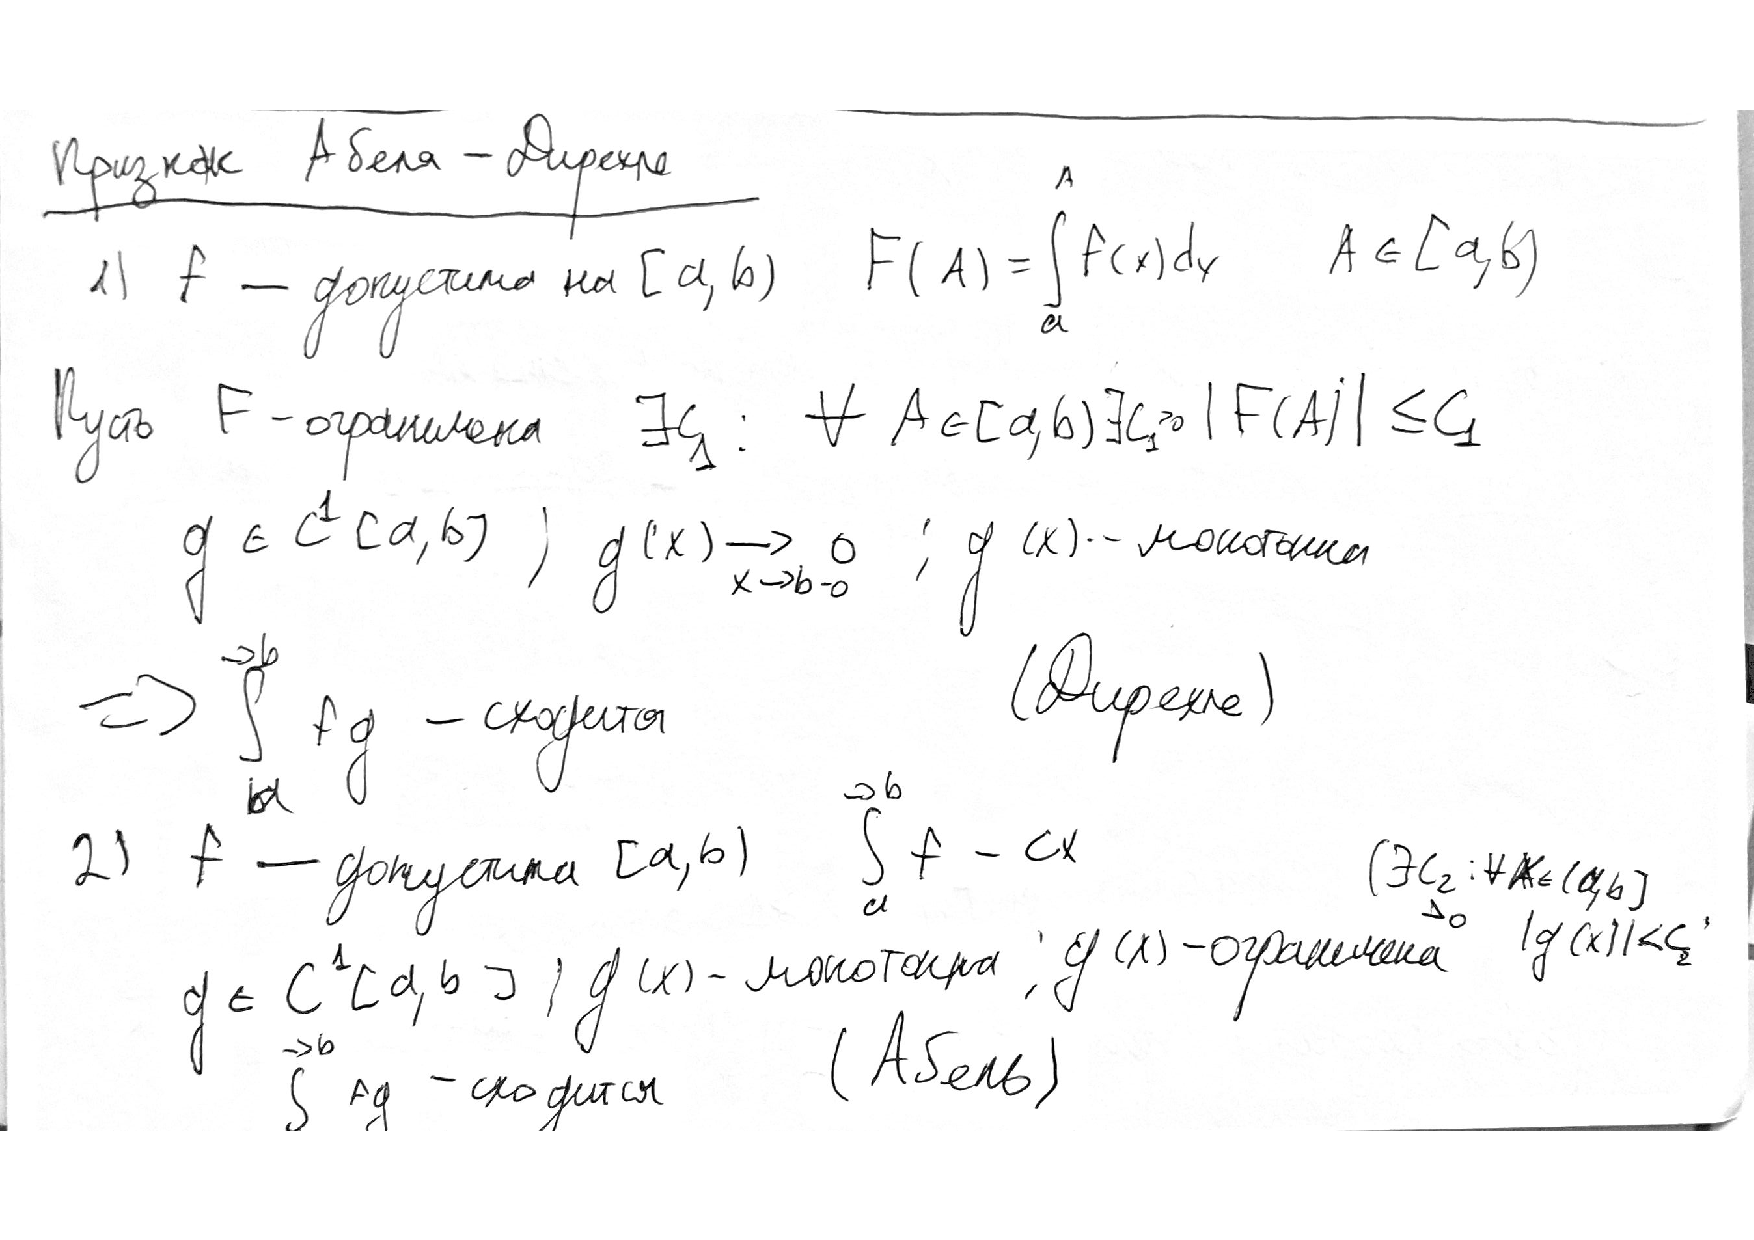
\includepdf[pages={-}]{../images/Abel-Direhle.pdf}

\subsubsection{Интеграл Дирихле\texorpdfstring{$^2$}{}}

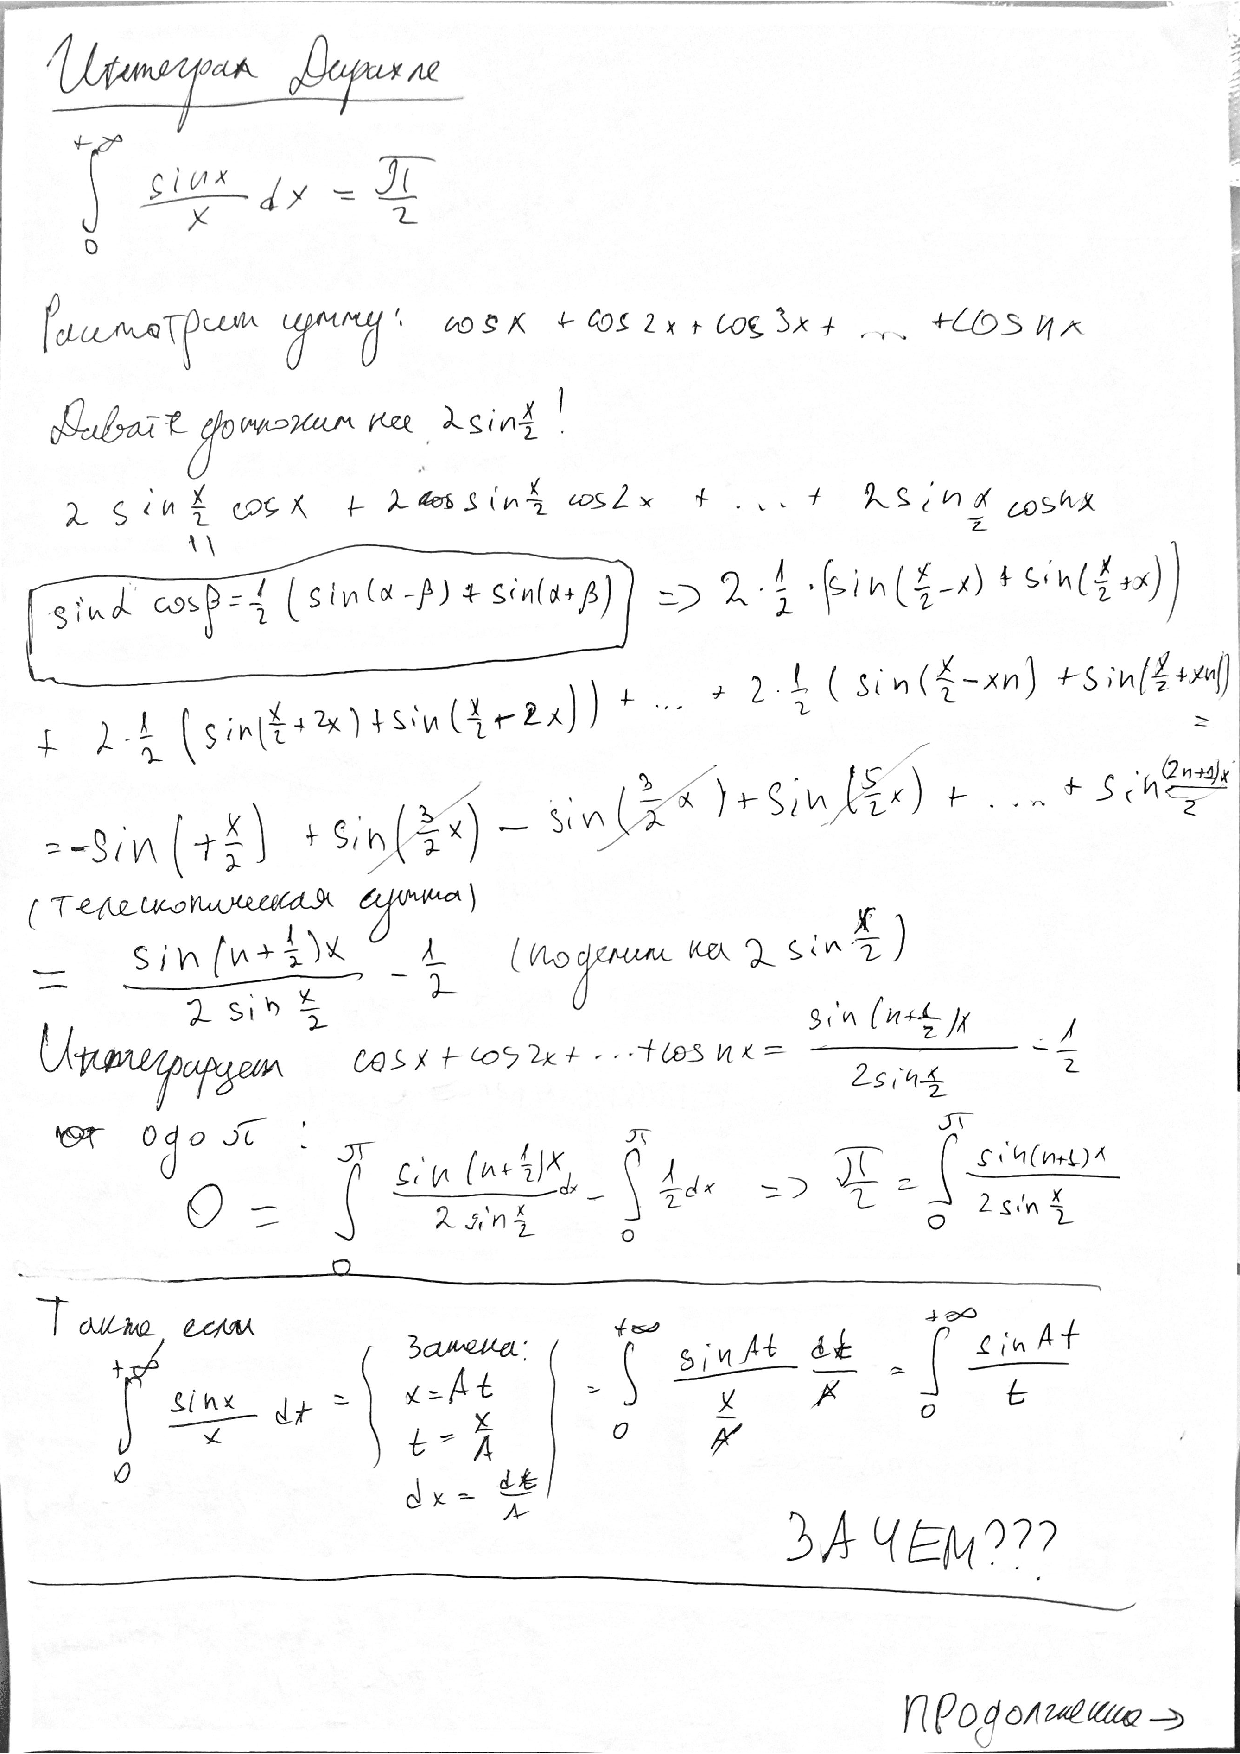
\includepdf[pages={-}]{../images/int_Dir.pdf}

\subsubsection{Неравенство Йенсена для интегралов\texorpdfstring{$^1$}{}}
\subparagraph{Формулировка}
$f: \langle A, B \rangle \rightarrow \mathbb{R}$ выпуклая, непрерывная.

$x: [a, b] \rightarrow \langle A, B \rangle$, непрерывная.

$\alpha: [a, b] \rightarrow \mathbb{R}_+$, непрерывная. $\int_a^b \alpha(t) \D t = 1$

$$
f(\int_a^b x(t) \alpha(t) \D t) \le \int_a^b \alpha(t) f(x(t)) \D t
$$


\subparagraph{Доказательство}
Тупо везде подставляем вместо сумм интеграл. ФСЁ!


Пользуясь выпуклостью, мы можем провести опорную прямую такую, что $f(x)$ будет выше этой прямой. Нас интересует прямая в точке $x^* := \int_a^b \alpha(t) x(t) \D t$ по условию. Но сначала надо убедиться, что точка лежит в $\langle a, b \rangle$:
$$
m := \inf_{t\in [a, b]} x(t)
$$
$$
M := \sup_{t\in [a, b]} x(t)
$$
$$
a \le m \le \int_a^b x(t) \alpha(t) \D t \le \int_a^b M \cdot \alpha(t) \D t = M \int_a^b \alpha(t) \D t = M \le b
$$

Теперь проводим опорную прямую:
$$
f(x^*) = kx^* + b = k \cdot \int_a^b \alpha(t) x(t) \D t + b = \int_a^b \alpha(t) \cdot k \cdot x(t) \D t + \int_a^b b \cdot \alpha(t) \D t = \int_a^b \alpha(t) (k \cdot x(t) + b) \D t \le \int_a^b \alpha(t) f(x(t)) \D t
$$
Note: $b = \int_a^b\alpha(t) \cdot b \D t$, так как сумма $\alpha_i = 1$

\subsubsection{Неравенство Коши (для сумм и для интегралов)\texorpdfstring{$^2$}{}}
\paragraph{Неравенство для сумм}
\textit{Формулировка}

$a_i > 0; \frac{1} {n} \sum a_i \geq \sqrt[n]{a_1 \ldots a_n}$
\begin{proof}
Напишем неравенство Йенсена для $\alpha_i = \frac{1} {n}; f(x) = \ln{x}$ - вогнутой:
\begin{align*}
\ln{\left(\frac{1} {n} a_1 + \frac{1} {n} a_2 + \ldots +  \frac{1} {n} a_n\right)} &\geq \frac{1} {n} \ln{a_1} + \frac{1} {n} \ln{a_2} + \ldots + \frac{1} {n} \ln{a_n}\\
\ln{\left(\frac{a_1 + a_2 + \ldots + a_n} {n} \right)} &\geq \frac{1} {n}\ln{(a_1 a_2 \dots a_n)}\\
\ln{\left(\frac{a_1 + a_2 + \ldots + a_n} {n} \right)} &\geq \ln{(a_1 a_2 \dots a_n)}^\frac{1} {n}
\end{align*}
Осталось только проэкспоненцировать получившееся неравенство:
\begin{equation*}
\frac{a_1 + a_2 + \ldots + a_n} {n} \geq \sqrt[n] {a_1 a_2 \dots a_n}
\end{equation*}
\end{proof}

\paragraph{Неравенство для интегралов}
\textit{Формулировка}

Пусть $f \in C[a, b], f > 0$. Тогда 
\begin{equation*}
exp\left(\frac{1} {b - a} \int_a^b \ln{f}\right) \leq \frac{1} {b - a} \int_a^b f
\end{equation*}
\begin{proof}
Рассмотрим интегральное неравенство Йенсена:
\begin{equation*}
f(\int_a^b x(t) \alpha(t) \D t) \le \int_a^b \alpha(t) f(x(t)) \D t
\end{equation*}
для $f(x) = \ln{x}$ - вогнутой, непрерывной. $\alpha(t) = \frac{1} {b - a} = const$. Видно, что $\int_a^b \alpha(t) \D t = 1$. Итого:
\begin{align*}
\ln{\left(\int_a^b x(t) \frac{1} {b - a} \D t\right)} &\geq \int_a^b \frac{1} {b - a} \ln{x(t)} \D t\\
\ln{\left(\frac{1} {b - a} \int_a^b x(t)\D t\right)} &\geq\frac {1}{b - a} \int_a^b \ln{x(t)} \D t
\end{align*}
Остается проекспоненцировать и получить требуемое неравенство:
\begin{equation*}
exp\left(\frac{1} {b - a} \int_a^b \ln{x(t)} \D t\right) \leq \frac{1} {b - a} \int_a^b x(t) \D t
\end{equation*}
\end{proof}

\subsubsection{Неравенство Гельдера для сумм\texorpdfstring{$^2$}{}}
\textit{Формулировка}

Пусть, $p > 1, q: \frac{1} {p} + \frac{1} {q} = 1 \Leftrightarrow q = \frac{p} {p - 1}$
$a_1, a_2, \dots, a_n, b_1, b_2, \dots, b_n > 0$
Тогда
\begin{equation*}
\sum a_i b_i \leq \left(\sum a_i\right)^\frac{1}{p} \left(\sum b_i\right)^\frac{1} {q}
\end{equation*}
\begin{proof}
Возьмем $x^p$ - строго выпуклая $\Leftrightarrow$ по неравенству Йенсена 
\begin{equation*}
\left(\sum \alpha_i x_i\right)^p \leq \sum \alpha_i x_i^p
\end{equation*}
Положим
\begin{align*}
\alpha_i :&= \frac{b_i^q} {\sum b_j^q}\\
x_i &= a_i b_i^{-\frac {1} {p - 1}} \sum b_j^q
\end{align*}
Тогда 
\begin{align*}
\sum \alpha_i x_i &= \sum \frac{b_i^q} {\sum b_j^q} a_i b_i^{-\frac {1} {p - 1}} \sum b_j^q = \\
&= \sum a_i b_i^{\frac{p} {p - 1} - \frac{1} {p - 1}} = \sum a_i b_i\\
\sum \alpha_i x_i^p &= \sum \frac{b_i^q} {\sum{b_j^q}} a_i^p b_i^{-\frac{p} {p - 1}}\left( \sum b_j^q\right) ^{p - 1} = \\
&= \sum a_i^p b_i^0 \left(\sum b_j^q\right)^{p - 1} = \left(\sum b_j^q\right)^{p - 1} \sum a_i^p
\end{align*}
Подставляем полученные выражения в неравенство Йенсена:
\begin{equation*}
\left(\sum a_i b_i\right)^p \leq \left(\sum b_j^q\right)^{p - 1} \sum a_i^p
\end{equation*}
Возводим обе части в степень $\frac{1} {p}$ и получаем требуемое неравенство:
\begin{equation*}
\sum a_i b_i \leq \left(\sum a_i^p\right)^\frac{1} {p} \left(\sum b_j^q\right)^\frac{1} {q}
\end{equation*}
\end{proof}

\subsubsection{Неравенство Минковского\texorpdfstring{$^2$}{}}
\textit{Формулировка}

Пусть, $p \geq 1$. Тогда
\begin{equation*}
\left(\sum(a_i + b_i)^p\right)^\frac{1} {p} \leq \left(\sum a_i^p\right)^\frac{1} {p} + \left(\sum b_i^p\right) ^\frac{1} {p}
\end{equation*}
\begin{proof}
Отображение $(x_1, x_2, \dots, x_n) \mapsto \left( \sum |x_i|^p\right)^\frac{1} {p}$ является нормой, т.е. выполняется неравенство треугольника:
\begin{equation*}
\left( \sum|a_i + b_i|^p\right)^\frac{1} {p} \leq  \left( \sum |a_i|^p\right)^\frac{1} {p} + \left( \sum |b_i|^p\right)^\frac{1} {p}
\end{equation*}
При $p = 1$ - очевидно.
Пусть $p > 1$, будем рассматривать только положительные $a_i, b_i$, все остальные будем сводить к ним.

Рассмотрим 
\begin{equation*}
\sum |a_i| |a_i + b_i|^{p - 1}, \qquad \sum|b_i| |a_i + b_i|^{p - 1}
\end{equation*}
Неравенство Гёльдера делает бррррр:
\begin{equation*}
\sum |a_i| |a_i + b_i|^{p - 1} \leq \left(\sum (a_i)^p\right)^\frac{1} {p} \left(\sum(a_i + b_i)^{(p - 1) * q}\right)^\frac{1} {q} = \left(\sum (a_i)^p\right)^\frac{1} {p} \left(\sum (a_i + b_i)^p\right)^\frac{1} {q}
\end{equation*}
Аналогично поступаем с $\sum |a_i| |a_i + b_i|^{p - 1} $ и складываем:
\begin{equation*}
\sum |a_i + b_i|^p \leq \sum |a_i + b_i| ^{p - 1} |a_i + b_i| \leq \left(\left(\sum|a_i^p|\right)^\frac{1} {p} + \left(\sum|b_i|^p\right)^\frac{1} {p}\right) \left(\sum|a_i + b_i|^p\right)^\frac{1} {q}
\end{equation*}
Делим обе части уравнения на $\left(\sum|a_i + b_i|^p\right)^\frac{1} {q}$:
\begin{align*}
\left(\sum|a_i + b_i|^p\right) ^{1 - \frac{1} {q}} &\leq \left(\sum|a_i|^p\right)^\frac{1} {p} + \left(\sum|b_i|^p\right)^\frac{1} {p}\\
\left(\sum|a_i + b_i|^p\right) ^\frac{1} {p} &\leq \left(\sum|a_i|^p\right)^\frac{1} {p} + \left(\sum|b_i|^p\right)^\frac{1} {p}
\end{align*}
\end{proof}

\subsubsection{Свойства рядов: линейность, свойства остатка, необх. условие сходимости, критерий Больцано--Коши\texorpdfstring{$^1$}{}}
\paragraph{Линейность}
$\sum a_n, \sum b_n$ сходятся, $c_n = a_n + b_n \Rightarrow \sum c_n$ сходится, $\sum c_n = \sum a_n + \sum b_n$

$\rhd$
$$
c_n = a_n + b_n \Rightarrow S_N^c = S_N^a + S_N^b
$$
$\lhd$

$\sum a_n$ сходится $\Rightarrow \forall \alpha \in \mathbb{R} \quad \sum \alpha a_n$ сходится, $\sum \alpha a_n = \alpha \cdot \sum a_n$

$\rhd$
$$
S_N^{\alpha a} = \alpha a_1 + \alpha a_2 \ldots \alpha a_N = \alpha (a_1 + a_2 + \ldots + a_N) = \alpha S_N^a \in \mathbb{R}
$$
$\lhd$
\paragraph{Свойства остатка}
\begin{enumerate}
    \item $\sum_{k=1}^{+\infty} a_k$ сходится $\Rightarrow \forall N \quad R_N$ сходится.
    
    $\rhd$
    Рассмотрим частичные суммы:
    $$
    S_N^a = \sum_{k=1}^N a_k = \sum_{k=1}^m a_k + \sum_{k=m+1}^N a_k
    $$
    При $n \rightarrow +\infty$
    $$
    \sum_{k=1}^{+\infty} a_k = \sum_{k=1}^m a_k + \sum_{k=m+1}^{+\infty} a_k
    $$
    $\lhd$
    
    \item $\exists N : R_N$ сходится $\Rightarrow \sum_{k=1}^{+\infty} a_k$ сходится.
    
    $\rhd$
    Такое же доказательство.
    $\lhd$
    
    \item $\sum_{k=1}^{+\infty} a_k$ сходится $\Leftrightarrow R_N \rightarrow 0$
    
    $\rhd$
    
    $\Rightarrow$

    Воспользуемся предыдущим доказательством, после предельного перехода мы получили выражение $\sum_{k=1}^{+\infty} a_k = \sum_{k=1}^m a_k + \sum_{k=m+1}^{+\infty} a_k$. $\sum_{k=1}^{+\infty} a_k$ ограничено, $\sum_{k=1}^m a_k$ ограничено. Причём $R_N = \sum_{k=m+1}^{+\infty} a_k$ и оно тоже ограничено. При $N \rightarrow +\infty$ всё больше членов ряда "отщипывается" в $\sum_{k=1}^m a_k$, следовательно, эта частичная сумма стремится к исходному ряду. В таком случае, $R_N$ ничего не остаётся, кроме как стремиться к 0, иначе доказанная выше сумма не выполнится.

    $\Leftarrow$
    
    Если мы рассматриваем последовательность остатков $R_N$ как какой-то объект, то там должна быть последовательность каких-то чисел, то есть они существуют, то есть существуют такие остатки в этой последовательности, которые будут сходиться к этим числам, то есть выполняется свойство 2.
    
    $\lhd$
\end{enumerate}

\paragraph{Необх. условие сходимости}
\subparagraph{Формулировка}
$\sum a_n$ сходится $\Rightarrow a_n \rightarrow 0$

\subparagraph{Доказательство}
$\sum a_n$ сходится $\Rightarrow$ последовательность $R_n \rightarrow 0$.
Это мы доказали выше. А теперь скажем $a_n = R_n - R_{n+1}$. $R_{n+1} \rightarrow 0$ так же, как и $R_n$.
Таким образом, $a_n \rightarrow 0$ как разность двух бесконечно-малых.

\paragraph{Критерий Больцано--Коши}
\label{КБК}
Хотим предложить какой-нибудь достаточный критерий для выяснения сходимости.
$$
\forall \varepsilon > 0 \exists N : \forall n > N \forall p > 0 \quad |a_n + a_{n+1} + \ldots + a_{n+p}| < \varepsilon
$$
Правое выражение эквивалентно следующему:
$$
|S_{n+p}-S_n| < \varepsilon
$$

При помощи этого мусора нетрудно доказать, что $\sum\frac{1}{n^p}$ расходится при $p \le 1$. Давайте просто предъявим $\varepsilon = 10^{-6}$, $n = N+1, p = N$. Там всё оценивается снизу по минимальному члену, $n$ сокращается и получается $\frac{1}{2} > \varepsilon$

\subsubsection{Признак Коши сходимости положительных рядов (pro)\texorpdfstring{$^1$}{}}
\subparagraph{Формулировка}
$$
\sum a_n \ge 0; \letus k_n = \sqrt[n]{a_n}
$$
Тогда:
\begin{enumerate}
    \item $\exists \overline{\lim} k_n < 1 \Rightarrow \sum a_n$ сходится
    \item $\exists \overline{\lim} k_n > 1 \Rightarrow \sum a_n$ расходится
    \item $\exists \overline{\lim} k_n = 1 \Rightarrow$ \Frowny
\end{enumerate}

\subparagraph{Доказательство}
Вспоминаем \nameref{КошиРяды}. Там сказаны чудесные слова про $k_n < q < 1$, а так же про бесконечное число элементов $\ge 1$. А теперь нам дали какие-то верхние пределы. Отлично! 

Вспоминаем \nameref{ТехВерхПредел}, а там у нас написано РОВНО ЭТО! В первом случае в качестве $\varepsilon$ предложим наше $q - k_n$, а во втором просто найдём какую-то точку $x : 1 < x < \overline{\lim} k_n$. И снова у нас будет выполняться тех. описание верхнего предела. Короче, мы в 2 строчки свелись к \nameref{КошиРяды}.

Если посмотреть на $\overline{\lim} k_n = 1$, то там всё грустно, так как предел не запрещает нашей функции быть в $\varepsilon$--окрестности как сверху от $1$, так и снизу. Так что признак не работает. 

Есть даже примеры: $\sum \frac{1}{n}$ и $\sum \frac{1}{n^2}$, один из них расходится, второй сходится, однако наша выбранная $k_n$ всё равно будет стремиться к $1$.


\subsubsection{Признак Даламбера сходимости положительных рядов\texorpdfstring{$^1$}{}}
\subparagraph{Формулировка}
$$
\sum a_n \ge 0; \letus D_n = \frac{a_{n+1}}{a_n}
$$
Тогда:
\begin{enumerate}
    \item Начиная с какого-то места $\exists q : D_n < q < 1$ ($q$ мы ввели чтобы потом сравнивать с ним, так как признак сравнения у нас строго $<1$ и с $1$ сравнивать неудобно) $\Rightarrow \sum a_n$ сходится
    \item Начиная с какого-то места $D_n \ge 1 \Rightarrow \sum a_n$ расходится.
\end{enumerate}
\paragraph{Pro версия:}
$\exists \lim D_n = D$
\begin{enumerate}
    \item $D < 1$ --- сходится
    \item $D > 1$ --- расходится
    \item $D = 1$ --- \Frowny
\end{enumerate}

\subparagraph{Доказательство}
\begin{enumerate}
    \item $\exists N_0 : \forall k \in \mathbb{N} \quad \frac{a_{N_0 + k + 1}}{a_{N_0 + k}} < q < 1$. Теперь распишем это как выражения $\frac{a_{N_0 + 1}}{a_{N_0}} < q, \frac{a_{N_0 + 2}}{a_{N_0 + 1}} < q, \ldots, \frac{a_{N_0 + k + 1}}{a_{N_0 + k}} < q$. 
    
    Главный трюк --- перемножим все эти выражения (левые и правые части) и у нас всё сократится: $\frac{a_{N_0+k+1}}{a_{N_0}} < q^k$. Выразим $a_{N_0 + k + 1}$: $a_{N_0 + k + 1} < q^k \cdot a_{N_0}$.
    
    Теперь устремим $k$ к $+\infty$ и получим, что получившееся неравенство --- это 2 ряда под признаком сравнения, при том, что справа у нас бесконечно убывающая геом. прогрессия, у которой по определению можно посчитать сумму, а значит она сходится. Слева неравенства у нас в таком случае будет записан остаток исходного ряда $R_{N_0 + 1}$. По признаку сравнения остаток сходится, а значит и исходный ряд сходится. 
    
    \item $q \ge 1$, а значит, что как минимум с этого места наш ряд не уменьшается, а значит он не может стремиться у нулю, а значит нет необходимого признака сходимости.
\end{enumerate}
\begin{enumerate}
    \item Доказывать нечего: выберем $\varepsilon$ такой, чтобы верхнее ограничение нашей последовательности было $< 1$, а это уже подходит под пункт 1 упрощённой версии.
    \item Аналогично
    \item Не работает, так как при $\varepsilon > 0$ у нас элементы в последовательности могут быть как $>1$ так и $<1$. Простейший контрпример: $\sum \frac{1}{n}$ и $\sum \frac{1}{n^2}$. У них у обоих $D = 1$
\end{enumerate}

\subsubsection{Признак Раабе сходимости положительных рядов\texorpdfstring{$^1$}{}}
\paragraph{Лемма (улучшенный признак сравнения)}
\subparagraph{Формулировка}
$\letus a_n, b_n > 0$
Если начиная с некоторого места
$$
\frac{a_{n+1}}{a_n} < \frac{b_{n+1}}{b_n}
$$
то
\begin{enumerate}
    \item $\sum b_n$ сходится $\Rightarrow \sum a_n$ сходится
    \item $\sum a_n$ расходится $\Rightarrow \sum b_n$ расходится
\end{enumerate}

\subparagraph{Доказательство}
$\exists N_0 : \forall k \in \mathbb{N} \quad \frac{a_{N_0 + k + 1}}{a_{N_0 + k}} < \frac{b_{N_0 + k + 1}}{b_{N_0 + k}}$. Теперь распишем это как выражения $\frac{a_{N_0 + 1}}{a_{N_0}} < \frac{b_{N_0 + 1}}{b_{N_0}}, \frac{a_{N_0 + 2}}{a_{N_0 + 1}} < \frac{b_{N_0 + 2}}{b_{N_0 + 1}}, \ldots, \frac{a_{N_0 + k + 1}}{a_{N_0 + k}} < \frac{b_{N_0 + k + 1}}{b_{N_0 + k}}$. 
    
Главный трюк --- перемножим все эти выражения (левые и правые части) и у нас всё сократится: $\frac{a_{N_0+k+1}}{a_{N_0}} < \frac{b_{N_0+k+1}}{b_{N_0}}$. Выразим $a_{N_0 + k + 1}$: $a_{N_0 + k + 1} < \frac{a_{N_0}}{b_{N_0}} \cdot b_{N_0+k+1}$.
    
Теперь устремим $k$ к $+\infty$ и получим, что справа неравенства у нас имеет место остаток ряда $R^{(b)}_{N_0+1}$, а слева тоже остаток $R^{(a)}_{N_0+1}$. Получается, мы свели эти все дроби к обычному признаку сравнения для рядов $\sum b_n$ и $\sum a_n$

\paragraph{Теорема}
\subparagraph{Формулировка}
$\letus a_n > 0$
\begin{enumerate}
    \item Начиная с некоторого места $n(\frac{a_n}{a_{n+1}} - 1) \ge r > 1 \Rightarrow \sum a_n$ сходится. Вот тут может быть больно: дробь записана вверх ногами, ещё и все неравенства перевёрнуты и ещё сравнение в обоих случаях нестрогое.
    \item Начиная с некоторого места $n(\frac{a_n}{a_{n+1}} - 1) \le 1 \Rightarrow \sum a_n$ расходится. 
\end{enumerate}

\subparagraph{Доказательство}
\begin{enumerate}
    \item 
    Итак, здесь всё сложно. Сначала давайте возьмём эталонный ряд, про который мы всё хорошо знаем и прогоним его в предельном переходе через формулу из формулировки: 
    $$
    \lim n\left(\frac{\frac{1}{n^S}}{\frac{1}{(n+1)^S}} - 1\right) = \lim n\left(\frac{n^S(1 + \frac{1}{n})^S}{n^S} - 1\right) = \lim n\left(\left(1 + \frac{1}{n}\right)^S - 1\right) = n\cdot S \frac{1}{n} = S
    $$
    Это всё значит, что мы можем взять наш эталонный ряд в такой хитровыебанной форме и с ним сравнивать то, что нам дают. Конкретно тут мы хотим подобрать такое $S$, чтобы оно лежало между $r$ и $1$. Слава Аллаху, это возможно. Разумеется, тогда мы выберем такое $\varepsilon$, что с некоторого места ВЕСЬ целиком эталонный ряд будет лежать между $r$ и $1$. Тогда мы сможем тупо сравнить эталонный ряд с тем, что нам дали по лемме выше. 
    
    Запишем что мы только что доказали:
    $$
    1 < n\left(\frac{\frac{1}{n^S}}{\frac{1}{(n+1)^S}} - 1\right) < r \le n\left(\frac{a_n}{a_{n+1}} - 1\right)
    $$
    Теперь разделим на $n$, прибавляем 1 и получаем красивое:
    $$
    \frac{\frac{1}{n^S}}{\frac{1}{(n+1)^S}} < \frac{a_n}{a_{n+1}}
    $$
    Ой, всё перевёрнуто((, ну ок:
    $$
    \frac{a_{n+1}}{a_n} < \frac{\frac{1}{(n+1)^S}}{\frac{1}{n^S}} 
    $$
    Итак, триумфальное шествие: по лемме если правая часть неравенства сходится, то сходится и левая. А мы знаем, что она (правая) сходится только при $S > 1$. А у нас $1 < S < r$, то есть мы подогнали всё так, что доказали сходимость. ЧТД.
    
    \item
    И вот тут мы наконец узнаем откуда взялось магическое $n(\frac{a_n}{a_{n+1}} - 1)$:
    $$
    n(\frac{a_n}{a_{n+1}} - 1) \ge 1 \Leftrightarrow \frac{a_n}{a_{n+1}} \ge \frac{1}{n} + 1 = \frac{1 + n}{n} = \frac{\frac{1}{n}}{\frac{1}{n + 1}}
    $$
    Оказывается, всё это время в этом выражении было зашито сравнение нашего ряда по нашей лемме с любимым эталонным рядом. Итого имеем:
    $$
    \frac{\frac{1}{n+1}}{\frac{1}{n}} \le \frac{a_{n+1}}{a_n}
    $$
    То есть если ряд слева расходится, то и справа расходится. А слева у нас спрятан ряд $\sum \frac{1}{n^1}$, то есть он как раз расходится.
\end{enumerate}

\paragraph{Pro}
Аналогично, как в Даламбере:
$$
\lim n\left(\frac{a_n}{a_{n+1}} - 1\right) = r
$$
\begin{enumerate}
    \item $r > 1 \Rightarrow \sum a_n$ сходится
    \item $r < 1 \Rightarrow \sum a_n$ расходится
    \item $r = 1 \Rightarrow$ \Frowny. Контрпример: ряды $\sum \frac{1}{n\ln n}$ и $\sum \frac{1}{n\ln^2 n}$
\end{enumerate}


\subsubsection{Интегральный признак Коши сходимости числовых рядов\texorpdfstring{$^1$}{}}
\subparagraph{Формулировка}
$\letus f: [1, +\infty) \rightarrow \mathbb{R}_+$ непрерывная, монотонная.

Тогда
$$
\sum_{k=2}^{+\infty} f(k) \,\text{сходится вместе с}\, \int_1^{+\infty}f(x)\D x
$$

\subparagraph{Доказательство}
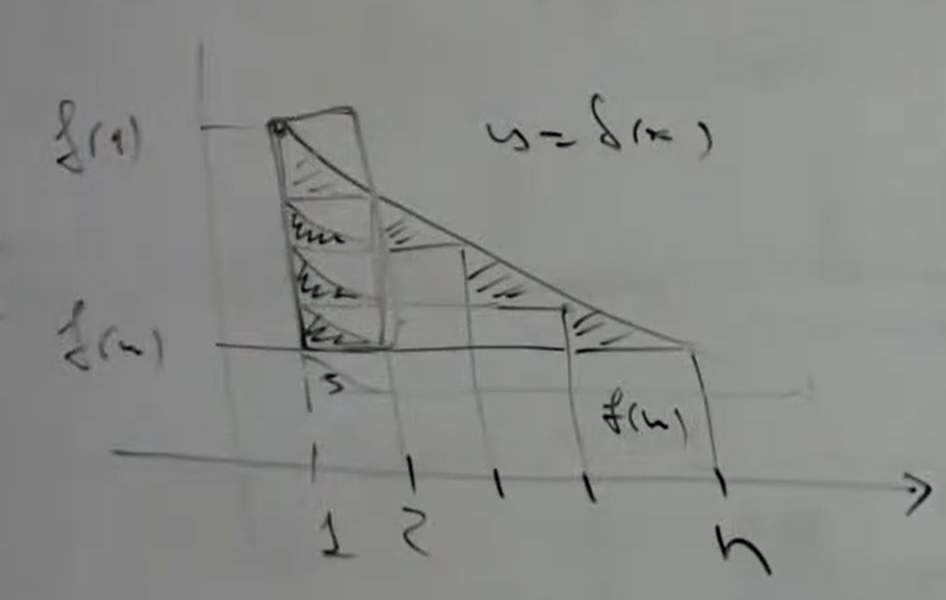
\includegraphics[]{../images/intkoshi.png}

Разбиение здесь единичное, так что ни на что не умножаем, зато мы тут видим, что мы можем достроить неучтённую в Римановой сумме часть функции до прямоугольника по левой стороне каждого отрезка (так как функция монотонно убывает). Сумма таких прямоугольников будет $|f(1) - f(n)|$ где $n$ --- правая граница границы интегрирования/частичной суммы, которую мы фиксируем.

Итак, мы можем записать всё это вот так:
$$
\left| \sum_{k=2}^n f(k) - \int_1^n f(x) \D x \right| \le |f(1) - f(n)|
$$
Для монотонно возрастающей функции всё симметрично.

Отсюда можно выразить частичную сумму
$$
S_n = \int_1^n f(x) \D x + \delta_n, |\delta_n| \le |f(1) - f(n)|
$$
$\delta_n$ --- это наша добавка--разница между суммой и интегралом.

Сходимость ряда будет следовать из существования + конечности предела этого предела при $n\rightarrow +\infty$. Если с влиянием на его конечность интеграла всё понятно, то остаётся только разобраться с влиянием на ответ $\delta_n$.

Заметим, что $\delta_n$ монотонно растёт в одну фиксированную сторону, ввиду монотонности исходной функции. Может ли он быть бесконечным? Очевидно, ввиду наших ограничений на функцию, в частности, непрерывности, бесконечным он может стать только если сама функция стремится в неограниченна, а следовательно, её интеграл тоже будет бесконечным, а значит этот частный случай никак не влияет на ответ. В остальных случаях $\delta_n$ конечная ввиду ограниченности $f$, а значит не влияет на сходимость ряда при предельном переходе.


\section{Период Кайнозойский}
\subsection{Важные определения}
\subsubsection{Сходимость последовательности в \texorpdfstring{$\mathbb{R}^m$}{R\^m}, покоординатная сходимость\texorpdfstring{$^1$}{}}
Последовательность сходится в $\mathbb{R}^m  \Leftrightarrow$ есть покоординатная сходимость.

Когда пишем последовательности в $\mathbb{R}^m$, мы пишем индекс сверху в скобках, а снизу пишем координату.
$$
x^{(n)} \rightarrow a \in \mathbb{R}^m \Leftrightarrow \left\{\begin{array}{c}
     x^{(n)}_1 \underset{n\rightarrow+\infty}{\longrightarrow} a_1 \\
     \vdots \\
     x^{(n)}_m \underset{n\rightarrow+\infty}{\longrightarrow} a_m \\
\end{array}\right.
$$

\subsubsection{Предельная точка, замкнутое множество, замыкание\texorpdfstring{$^1$}{}}
Тут тоже без новостей:

Предельная точка --- точка, любая проколотая окрестность которой непуста.

Замкнутое множество --- множество, включающее все свои предельные точки (или просто дополнение к открытому).

Замыкание --- минимальное по включению замкнутое множество, включающее исходное.

\subsubsection{Отображение бесконечно малое в точке\texorpdfstring{$^2$}{}}

$\varphi : E \subset R^m \rightarrow R^l$ --- \textit{отображение}

$x_0 \in E$ --- \textit{предельная} точка $E$

$\varphi$ является \textit{бесконечно малым в точке} $x_0$, если $\varphi(x) \rightarrow_{x \rightarrow x_0} 0$

\subsubsection{Отображение, дифференцируемое в точке\texorpdfstring{$^2$}{}}

$F : E \subset \mathbb{R}^m \rightarrow \mathbb{R}^l, a \in Int(E)$

Если $\exists L : \mathbb{R}^m \rightarrow \mathbb{R}^l$ --- линейный оператор, $\exists \alpha : E \rightarrow \mathbb{R}^l$ --- бесконечно малое, то $F(x)$ дифференцируемо в точке $a$:

$$
F(a+h)=F(a)+Lh+\alpha \cdot h, h \rightarrow 0
$$
$$
F(a+h)=F(a)+L \cdot h+o(h)
$$
$$
x:=a+h
$$
$$
F(x)=F(d)+L \cdot(x-a)+o(|x-a|)
$$

\subsubsection{Производный оператор, матрица Якоби, дифференциал\texorpdfstring{$^2$}{}}

Из определения выше, $L$ --- производный оператор.
В точке $a$ записывается следующим образом: $F^\prime(a)$


Матрица, задающая производный оператор, называется матрицей Якоби (по сути своей, матрица производных по всем переменным в этой точке).

Дифференциал функции $F$ в точке $a$ --- $F^\prime(x)h$, где $h \rightarrow 0$

\subsubsection{Частные производные\texorpdfstring{$^2$}{}}

$F : E \subset \mathbb{R}^m \rightarrow \mathbb{R}^1 $

Фиксируем какую-нибудь переменную $x_k, 1 \le k \le m$, $a \in Int(E)$

Заведём себе функцию $\varphi_k(t) := f(a_1, a_2, \ldots, a_{k - 1}, t, a_{k + 1}, \ldots, a_m)$, причём $t \in U(a)$.

\[\lim_{s \rightarrow 0} \frac{\varphi_k(t + s)}{\varphi_k(t)}\] --- частная производная $F$ в точке
$a$ по $x_k$. Причём \textit{частная} от слова \textit{partial}, а не от \textit{private}.

Также немаловажным будет отметить, как их обозначают. $\pdv{f}{x_1}{x_2}$ --- это производная 2-го порядка, причём сначала мы дифференцировали по $x_2$, а потом уже по $x_1$. Однако, нам не важно, в каком порядке дифференцировать, что доказывается далее. Причём, через неважность для перестановки 2х спокойно выражаются и перестановки любой длины, через транспозиции (привет, ДМ 1 сем!).



\subsubsection{Формула Тейлора (различные виды записи)\texorpdfstring{$^2$}{}}

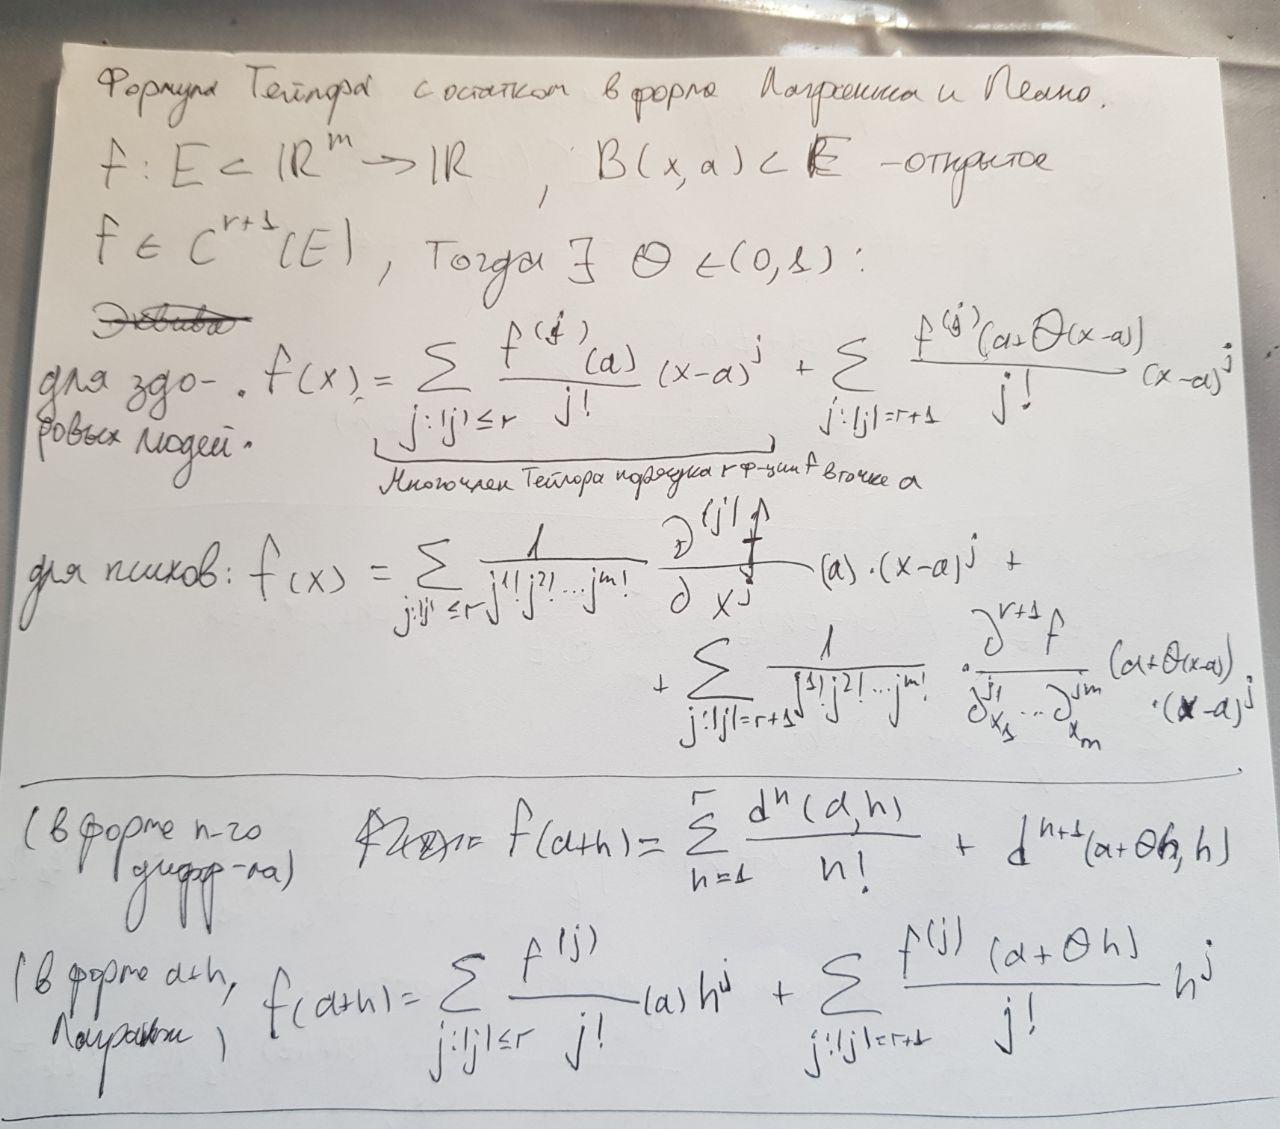
\includegraphics[width=\textwidth]{../images/teilor1.jpg}
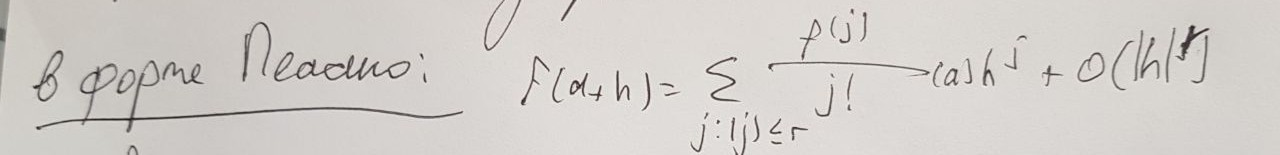
\includegraphics[width=\textwidth]{../images/teilor2.jpg}

\newpage
\subsection{Определения}

\subsubsection{Скалярное произведение, евклидова норма и метрика в \texorpdfstring{$\mathbb{R}^m$}{R\^m}\texorpdfstring{$^1$}{}}
$$
\letus a, b \in \mathbb{R}^m
$$
\paragraph{Скалярное произведение}
$$
\langle a, b \rangle := \sum a_i \cdot b_i
$$

\paragraph{Евклидова норма}
$$
|a| = \sqrt{\langle a, a\rangle}
$$

\paragraph{Метрика в \texorpdfstring{$\mathbb{R}^m$}{R\^m}}
$$
\rho(a, b) = |a - b|
$$
Вообще ничего нового, просто напоминалка, получается. 

\subsubsection{Окрестность точки в \texorpdfstring{$\mathbb{R}^m$}{R\^m}, открытое множество\texorpdfstring{$^1$}{}}
Открытое множество --- множество, все точки которого внутренние (входят вместе с какой-то окрестностью)

Окрестность точки --- какое-то открытое множество, включающее эту точку. Обозначается $U(a)$. Может быть проколото, в этом случае сама точка удаляется. 

Шар $B(a, r)$ --- множество всех точек, для которых верно $\rho(x, a) < r$.

$\varepsilon$--окрестность точки --- открытый шар $B(a, \varepsilon)$

\subsubsection{Компактность, секвенциальная компактность, принцип выбора Больцано-Вейерштрасса\texorpdfstring{$^1$}{}}
Компактное множество в $\mathbb{R}^m$ --- это замкнутое и ограниченное множество (ввиду полноты $\mathbb{R}^m$).

В $\mathbb{R}^m$ компактное множество секвенциально компактно, либо замкнуто + имеет конечную $\varepsilon$--сеть.

Секвенциальная компактность множества гласит, что в любой последовательности, заданной в множестве можно выбрать подпоследовательность, сходящуюся к точке в самом этом множестве.

Принцип выбора Больцано--Вейерштрасса почти про то же. В любой последовательности в ограниченном множестве можно выбрать сходящуюся подпоследовательность (предел не обязательно лежит в множестве, так что этого недостаточно для компактности!)

\subsubsection{Координатная функция\texorpdfstring{$^1$}{}}
$$
f: \mathbb{R}^m \rightarrow \mathbb{R}^l
$$
Такую функцию можно расписать как вектор координатных функций:
$$
x \mapsto f(x) = \left(\begin{array}{c}
     f_1(x) \\
     \vdots \\
     f_l(x)
\end{array} \right)
$$

\subsubsection{Двойной предел, повторный предел\texorpdfstring{$^1$}{}}
$\letus f: (x_1, x_2) \rightarrow \mathbb{R}, (a_1, a_2)$ --- предельная точка

\paragraph{Двойной предел}
На языке окрестностей (иначе зачем мы только что их вводили):
$$
\lim_{\begin{array}{c} x_1\rightarrow a_1 \\ x_2 \rightarrow a_2 \end{array}} f(x_1, x_2) = L \Leftrightarrow \forall U(L) \exists U(a_1) \exists U(a_2) : \forall x_1 \in \dot{U}(a_1) \cap D_1 \forall x_2 \in \dot{U}(a_2) \cap D_2 \quad f(x_1, x_2) \in U(L) 
$$
А ещё мы разрешили $a_1 \in \overline{\mathbb{R}}, a_2 \in \overline{\mathbb{R}}, L \in \overline{\mathbb{R}}$.

Мы нарисовали двойной предел... Добавить нечего.

\paragraph{Повторный предел}
Введём 
$$\phi(x_1) = \lim_{x_2 \rightarrow a_2} f(x_1, x_2)$$
Тогда можно определить предел
$$
\lim_{x_1\rightarrow a_1} \phi(x_1) = \lim_{x_1\rightarrow a_1} \lim_{x_2 \rightarrow a_2} f(x_1, x_2)
$$
Но если вы не прогуливали матан в 1 семестре, вы скажете, что тут как бы надо вообще гарантировать, что $\phi(x)$ возвращает что-то адекватное ($\in \mathbb{R}$, например) при всех $x \in D \setminus a_1$, иначе мы не сможем посчитать этот самый коварный наружный предел.

Вот то, что мы ввели вообще-то прозвали \textit{повторным пределом} в точке $(a_1, a_2)$.

\textit{Nota bene}: таким же образом мы имеем право ввести ещё и другой повторный предел, нарисовав композицию двух пределов в другом порядке (и даже получить другой ответ в некоторых случаях \Smiley)

\subsubsection{Предел по направлению, предел вдоль пути\texorpdfstring{$^1$}{}}
\paragraph{Предел по направлению}
Зададим прямую (направление) как $\phi(t) = a + t\cdot v$, где $a, v \in \mathbb{R}^m$. Физический смысл $a, b$ такой же как и в одномерном случае для начального сдвига и коэффициента наклона.

Тогда можно посчитать предел $\lim_{t\rightarrow 0}(\phi(t)) = \lim_{t\rightarrow 0}(a + t \cdot v)$. 

\paragraph{Предел вдоль пути}
$\letus E$ --- путь, проходящий через $a$ такой, что $[-\varepsilon, \varepsilon] \mapsto (x_1(t), x_2(t)), (x_1(0), x_2(0)) = a$

Тогда можно посчитать предел $\lim_{t\rightarrow 0} f(x_1(t), x_2(t))$. Не то, чтобы прям содержательно, но да.

\subsubsection{Линейный оператор\texorpdfstring{$^1$}{}}
Линейный оператор --- отображение $F: X \rightarrow Y$ (где $X, Y$ --- линейные пространства), которое имеет свойство линейности: $F(\alpha x + \beta y) = \alpha F(x) + \beta F(y)$.


$F: X \rightarrow \mathbb{R}^n$ договорились называть линейным функционалом

Для фиксированного множества $X, Y$ можно задать множество всех линейных операторов и обозначить как $Lin(x, y)$.

Договорились допускать операции над самими лин. операторами, которые сами по себе тоже являются лин. операторами в том же множестве $Lin$:
$$(F + G)(x) := F(x) + G(x)$$
$$(\alpha F)(x) := \alpha F(x)$$
$$F: X \rightarrow Y, G: Y \rightarrow Z \Rightarrow G(F): X \rightarrow Z$$


\subsubsection{\texorpdfstring{$o(h)$}{o(h)} при \texorpdfstring{$h \rightarrow 0$}{h -> 0}\texorpdfstring{$^2$}{}}

$\varphi : E \subset \mathbb{R}^m \rightarrow \mathbb{R}^l, $ 0 --- предельная точка $E$.

Можно задать нашу функцию $\varphi(h)$ двумя способами:
\begin{enumerate}
    \item $ \varphi(h)=o(h)$, при $ h \rightarrow 0 $
    
$ \frac{\varphi(h)}{|h|} \underset{h \rightarrow 0}{\longrightarrow} 0 $

    \item $ \exists \alpha(h) : E \rightarrow \mathbb{R}^l $ бесконечно малая при $ h \rightarrow 0 $
    
    $ \varphi(h)=|h| \cdot \alpha(h) $
\end{enumerate}

\subsubsection{Теорема о двойном и повторном пределах\texorpdfstring{$^1$}{}}
$\letus f: (x_1, x_2) \rightarrow \mathbb{R}$

Если
\begin{enumerate}
    \item $\exists \lim\limits_{\begin{array}{c} x_1\rightarrow a_1 \\ x_2 \rightarrow a_2 \end{array}} f(x_1, x_2) = L$
    \item $\forall x_1 \in D_1 \setminus \{a_1\} \exists$ конечный $\phi(x_1) := \lim\limits_{x_2\rightarrow a_2} f(x_1, x_2)$
\end{enumerate}
Тогда $\exists \lim\limits_{x_1\rightarrow a_1} \phi(x_1) = L$

Был показательный пример с $\frac{x_1+x_2}{x_1-x_2}$, в котором разные повторные пределы давали разный ответ. Так вот, по этой теореме мы сможем убедиться, что тут не выполняется первый пункт, а значит повторный предел не существует.

\subsubsection{Производная по направлению\texorpdfstring{$^2$}{}}

$f: E \subset \mathbb{R}^m \rightarrow \mathbb{R}, \dbl a \in Int(E), \dbl h \in \mathbb{R}^m$

Пусть $t \in \mathbb{R}, |h| = 1$ (такой вектор  называется направлением).

Тогда $\lim_{t \rightarrow 0}{\frac{f(a + th) - f(a)}{t}} = (\pdv{f}{d})(a)$ --- производная по направлению. 

\textit{Замечание}

Функция дифференцируема $\Rightarrow$ функция дифференцируема по любому вектору (направлению)

$\lim_{t \rightarrow 0}{\frac{f(a + th) - f(a)}{t}} = \lim_{t \rightarrow 0}{\frac{f^\prime_1(a)th + f^\prime_2(a)th + \ldots + f^\prime_m(a)th + o(t)}{t}} = f^\prime_1(a)h + f^\prime_2(a)h + \ldots + f^\prime_m(a)h = \langle \grad f, h \rangle$

\subsubsection{Градиент\texorpdfstring{$^2$}{}}

$f: E \subset \mathbb{R}^m \rightarrow \mathbb{R}, \dbl a \in Int(E), \dbl h \in \mathbb{R}^m$

$f(a + h) = f(h) + \langle L, h\rangle + o(|h|), h \rightarrow 0$

Вектор $L$ называется градиентом $f$ в точке $a$.

$L = \text{grad} f = \grad f$

\subsubsection{Мультииндекс и обозначения с ним\texorpdfstring{$^2$}{}}

Мультииндекс $k$ в $\mathbb{R}^m$ --- $(k_1, k_2, \ldots, k_m), \dbl k_i \in \mathbb{N} \setminus \{0\}$

Некоторые обозначения:

\begin{enumerate}
    \item $|k| = k_1 + k_2 + \ldots + k_m$ --- высота мультииндекса
    \item $k! = k_1!k_2!\ldots k_m!$
    \item $x^k = x^{k_1}x^{k_2}\ldots x^{k_m}$
\end{enumerate}

\subsubsection{\texorpdfstring{$n$}{n}-й дифференциал\texorpdfstring{$^2$}{}}

\textsc{Literally this: }
\[ d^n f = \sum_{j : |j| = n}{\frac{n! f^{(n)}}{j!}}(a)h^j \] ($n$-я сумма из леммы о нахождении производной сдвига (?))

Но можно расписать и по-другому, основываясь на выводе полиномиальной формулы (наивная версия):

\[d^n f = \sum_{i_1 = 1}^m \sum_{i_2 = 1}^m \dots \sum_{i_m = 1}^m \frac{\partial^n}{\partial^{j_1}{x_1}\partial^{j_2}{x_2}\ldots\partial^{j_m}{x_m}}(a)dx_1dx_2\ldots dx_m\]

Что тут происходит? Мы ищем производную $n$-го порядка, с какой-нибудь комбинацией переменных, по которым дифференцируем. А также отмечаем, по каким переменных шло дифференцирование, домножая на $dx_i$

\newpage
\subsection{Важные теоремы}

\subsubsection{Признак Лейбница\texorpdfstring{$^1$}{}}
\subparagraph{Формулировка}
$\letus \sum_{n=1}^{+\infty} (-1)^n C_n, C_n \ge C_{n+1} \ge 0$

Тогда
$$
C_n \rightarrow 0 \Rightarrow \sum_{n=1}^{+\infty} (-1)^n C_n
$$
сходится.

\subparagraph{Доказательство}
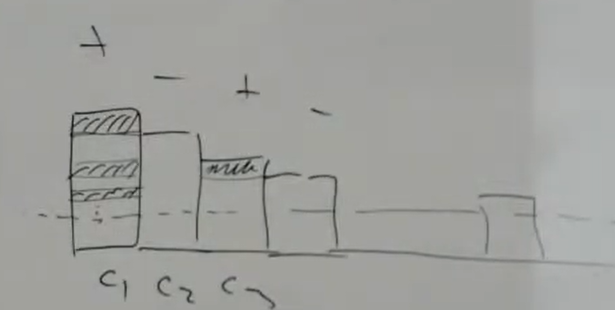
\includegraphics[]{../images/leibniz.png}

Будем попарно брать столбики с противоположными знаками и разницу между ними закрашивать. Заметим, что сумма всех этих "разниц" --- это и будет сумма ряда. А ещё она вся вписывается в первый столбец (очевидно, ввиду монотонности, на рисунке видно).

Но! В условии ещё что-то сказано про $C_n \rightarrow 0$. Так вот, если этого не соблюсти, то у нас произойдёт разночтение предела, т.к. можно будет взять частичные суммы до чётного члена, а также до нечётного. И вот если этот "последний" член окажется нечётным, то он нам добавит чего лишнего, а если предел неоднозначен, то его не существует. И вот, чтобы этого избежать, мы требуем, чтобы оно стремилось к $0$.


\subsubsection{Достаточное условие дифференцируемости\texorpdfstring{$^2$}{}}

\subparagraph{Формулировка: }

$f : E \subset \mathbb{R}^m \rightarrow \mathbb{R}, \dbl a \in Int(E)$

Пусть в окрестности $B(a, r)$ существуют конечные $f^\prime_1, \ldots, f^\prime_m$ и все они непрерывны в точке $a$. Тогда, $f$ дифференцируема в точке $a$.

\subparagraph{Доказательство: }

$\rhd$

Рассмотрим для $m = 2$, для остальных всё аналогично.

Возьмём разность $f(x_1, x_2) - f(a_1, a_2)$. Добавим и вычтем $f(a_1, x_2)$:

\[ = \left(f(x_1, x_2) - f(a_1, x_2)\right) + \left(f(a_1, x_2) - f(a_1, a_2)\right) = \]

Расписываем каждую скобку по теореме Лагранжа, переменные с шапочками --- это что-то среднее между иксом и ашкой:

\[ = f^\prime_{x_1}(\hat{x_1}, x_2)(x_1 - a_1) + f^\prime_{x_2}(a_1, \hat{x_2})(x_2 - a_2) = \]

Теперь добавим и вычтем $i \in \{1, 2\}, \dbl f^\prime_{x_i}(a_1, a_2)(x_i - a_i)$
\[ = f^\prime_{x_1}(a_1, a_2)(x_1 - a_1) + f^\prime_{x_2}(a_1, a_2)(x_2 - a_2) + \]

\[+ (x_1 - a_1)(f^\prime_{x_1}(\hat{x_1}, x_2) - f^\prime_{x_1}(a_1, a_2)) + (x_2 - a_2)(f^\prime_{x_2}(a_1, \hat{x_2}) - f^\prime_{x_2}(a_1, a_2))\]

Заметим, что $i \in \{1, 2\}, \dbl (x_i - a_i) \le |x_i - a_i|$ (нормы), а выражения в скобках --- бесконечно малые при $x \rightarrow a$.

В итоге, получили формулу дифференцирования, где слева стоит формула, справа линейная часть и бесконечно малая.

$\lhd$

\subsubsection{Дифференцирование композиции\texorpdfstring{$^2$}{}}

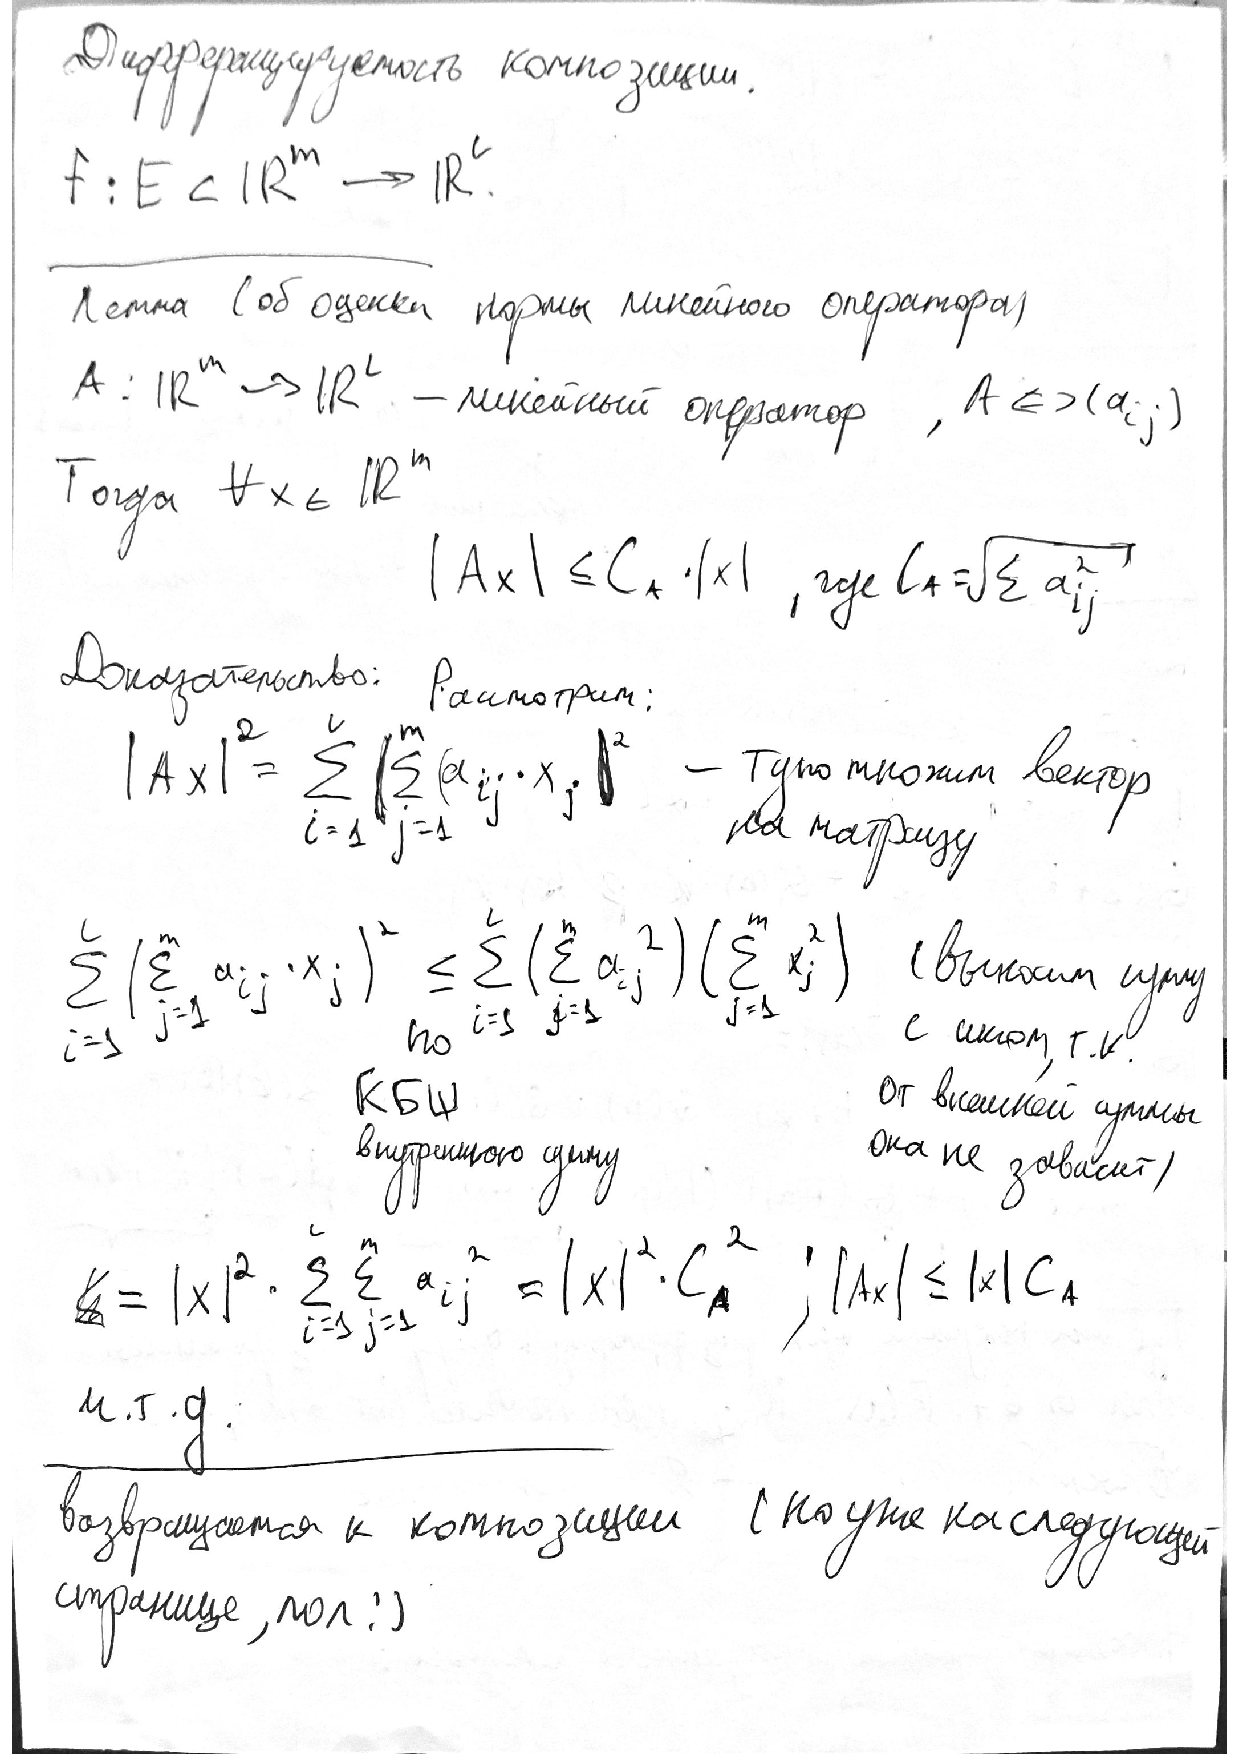
\includepdf[pages={-}]{../images/Diff_comp.pdf}

\subsubsection{Теорема Лагранжа для векторнозначных функций\texorpdfstring{$^2$}{}}

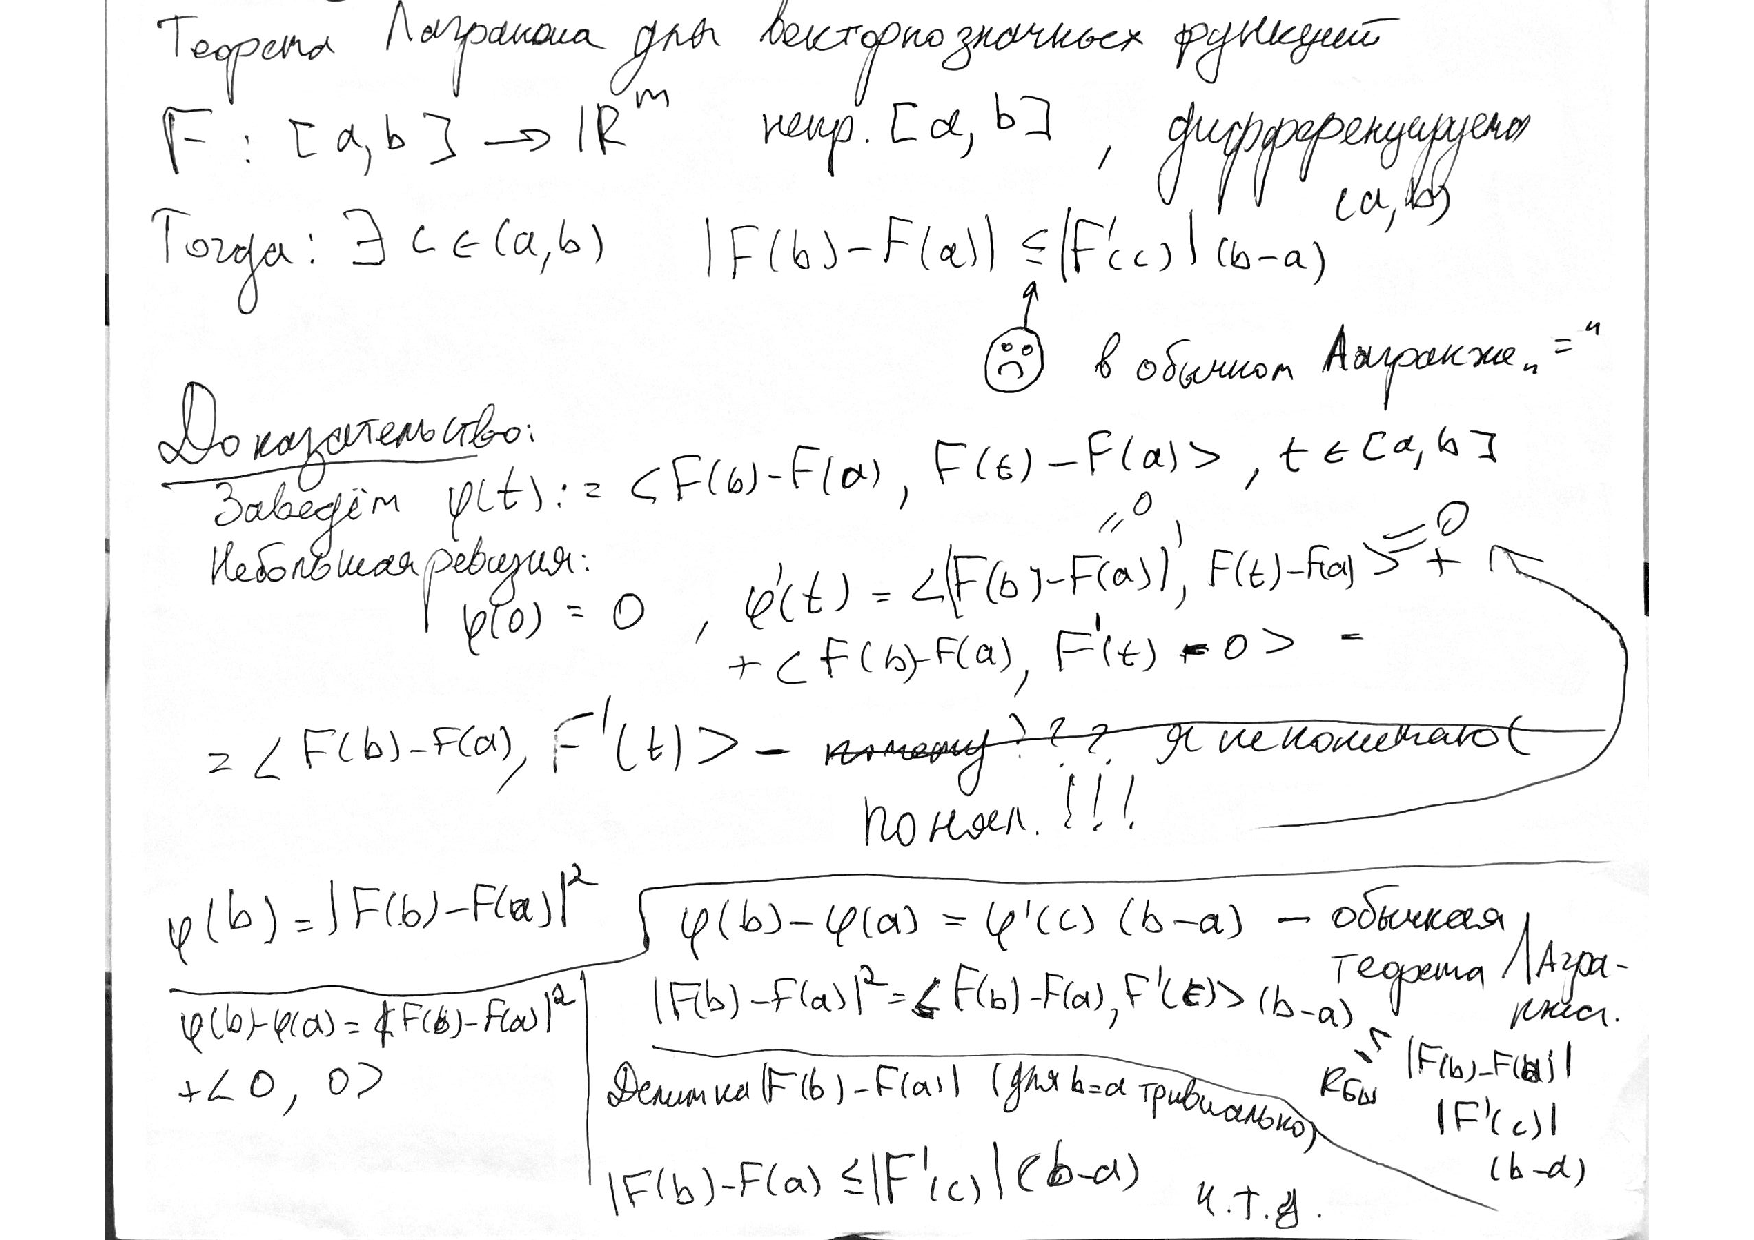
\includepdf[pages={-}]{../images/Lagr_Vect.pdf}

\subsubsection{Многомерная формула Тейлора (с остатком в форме Лагранжа и Пеано)\texorpdfstring{$^2$}{}}

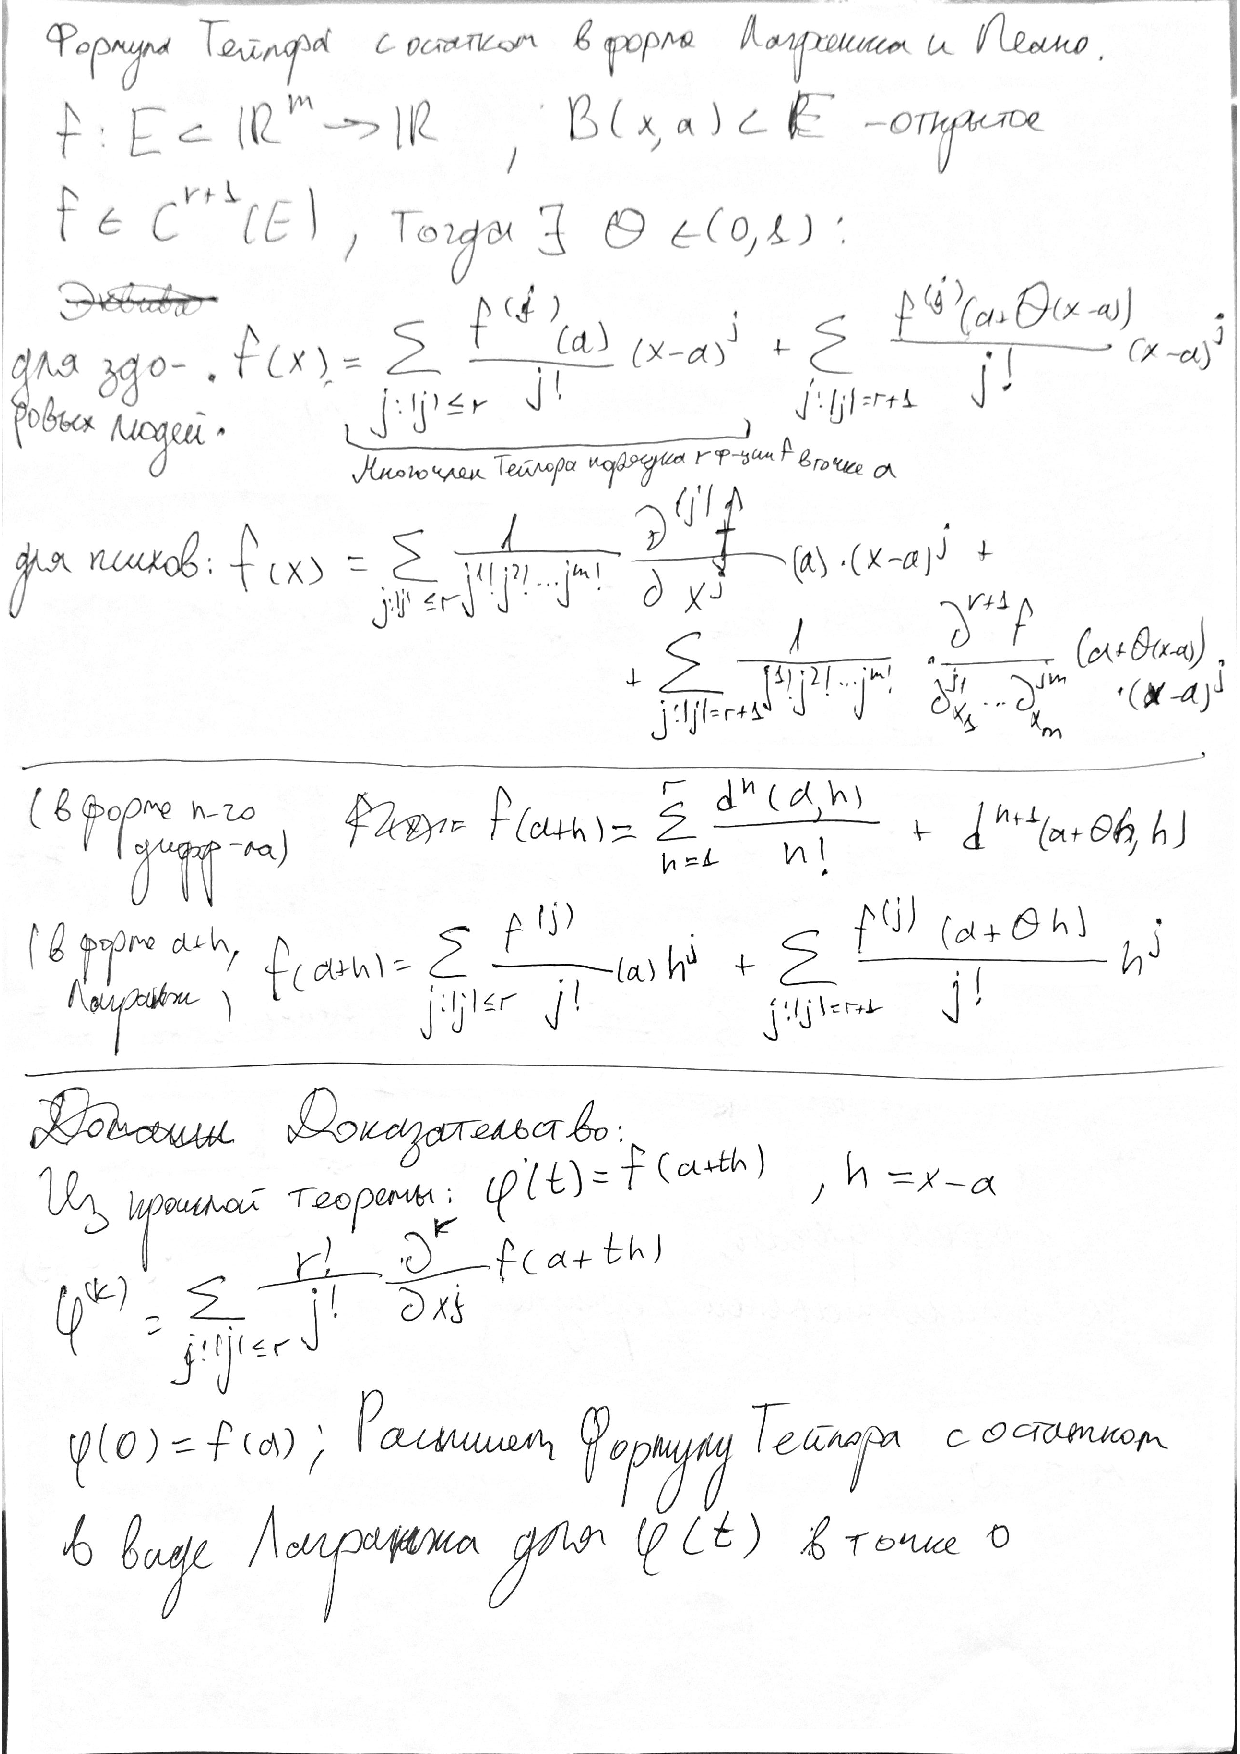
\includepdf[pages={-}]{../images/Form_Teilor.pdf}

\newpage
\subsection{Теоремы}

\subsubsection{Признаки Дирихле и Абеля сходимости числового ряда\texorpdfstring{$^1$}{}}
\paragraph{Преобразование Абеля (суммирование по частям)}
$$
A_n := \sum_{i=1}^n a_i
$$
$$
\sum_{k=1}^N a_k b_k = A_N b_N + \sum_{k=1}^{N-1} A_k (b_k - b_{k+1})
$$

\paragraph{Дирихле}
\subparagraph{Формулировка}
$\letus \sum_{n=1}^{+\infty} a_n b_n$
\begin{enumerate}
    \item $A_n$ ограничено, т.е. $\exists C_A : \forall n > 0 \quad |A_n| \le C_A$
    \item $b_n$ монотонно и $b_n \rightarrow 0$
\end{enumerate}
Если всё выполняется, ряд сходится. 

\subparagraph{Доказательство}
Запишем преобразование Абеля:
$$
\sum_{k=1}^N a_k b_k = A_N b_N + \sum_{k=1}^{N-1} A_k (b_k - b_{k+1})
$$
Здесь $A_N$ ограничено, $b_N$ б.м. $\Rightarrow A_N b_N \rightarrow 0$.

Остаётся доказать абсолютную сходимость $\sum_{k=1}^{N-1} A_k (b_k - b_{k+1})$:
$$
b_n \rightarrow 0 \Rightarrow \exists C_B : \forall n > 0 \quad |b_n| < C_B
$$
$$
\sum_{k=1}^{N-1} |A_k| |b_k - b_{k+1}| \le C_A \sum_{k=1}^{N-1} |b_k - b_{k+1}| = \pm C_A (b_k - b_{k+1} + b_{k+1} - b_{k+2} + \ldots + b_{N-1} - b_N) = \pm C_A (b_k - b_N) \le 2 \cdot C_A \cdot C_B
$$
Все числа здесь конечны, а значит ряд абсолютно сходится (а значит, просто тоже сходится), а значит в исходном преобразовании Абеля у нас все слагаемые сходятся, а значит сам представленный ряд сходится. 

\paragraph{Абель}
\subparagraph{Формулировка}
\begin{enumerate}
    \item $\sum_{n=1}^{+\infty} a_n$ сходится ($\Rightarrow \exists \lim_N \sum_{n=1}^{N} a_n = \alpha$)
    \item $b_n$ монотонно, $b_n$ ограничено
\end{enumerate}
Здесь требования к $a_n$ сильнее, а к $b_n$ слабее.
\subparagraph{Доказательство}
Вспоминаем, что у монотонной и ограниченной последовательности есть предел:
$$
\exists \lim b_n := \beta
$$
Далее нам надо сделать супер--мега--трюк, а именно прибавить и отнять от исходного ряда $\beta\sum_{n=1}^N a_n$:
$$
\sum_{n=1}^N a_n b_n = \beta\sum_{n=1}^N a_n + \sum_{n=1}^{N} a_n b_n - \beta\sum_{n=1}^N a_n = \beta\sum_{n=1}^N a_n + \sum_{n=1}^{N} a_n (b_n - \beta)
$$
При $N \rightarrow +\infty$ происходит предельный переход:
$$
\sum_{k=1}^{+\infty} a_k b_k = \beta\alpha + \sum_{n=1}^{+\infty} a_n (b_n - \beta)
$$
Левое слагаемое конечно, обратим внимание на правое: $\sum_{k=1}^{+\infty} a_k (b_k - \beta)$ сходится по признаку Дирихле, так как $a_k$ сходится $\Rightarrow a_k$ ограничено, $b_k \rightarrow \beta \Rightarrow b_k - \beta \rightarrow 0$, монотонность $b_k$ у нас остаётся по условию.

Таким образом, получившееся выражение тоже целиком сходится.


\subsubsection{Единственность производной\texorpdfstring{$^2$}{}}

\subparagraph{Формулировка: }

Производный оператор (если он существует) определён однозначно.

\subparagraph{Доказательство: }

$\rhd$

Краткий ответ: так как он вычисляется однозначно для каждого $u \in \mathbb{R}^m$.

Докажем этот удивительный аспект!

$F: E \subset \mathbb{R}^m \rightarrow \mathbb{R}^l$

\[F(a + h) = F(a) + Lh + o(h)\]

Пусть $h = tu$, где $t \in \mathbb{R}$. Причём, $|t| < \frac{r}{|u|}, B(a, r) \in E$ Тогда:

\[F(a + tu) = F(a) + tLu + o(t)\]
\[Lu = \frac{F(a + tu) - F(a)}{t} - \frac{o(t)}{t}\]
\[Lu = \lim_{t \rightarrow 0}{\frac{F(a + tu) - F(a)}{t}}\] --- однозначно определено!

$\lhd$

\subparagraph{Замечание (о дифференцируемости функции нескольких переменных): }

Логично, что $x \mapsto (x_1, x_2, \ldots, x_m) \Rightarrow f(x_1, x_2, \ldots, x_m)$. Поэтому в векторном виде можно записать дифференцируемость так:

\[F(x + a) = F(a) + L(x - a) + \Phi(x - a)|x - a|\]

\subsubsection{Лемма о дифференцируемости отображения и его координатных функций\texorpdfstring{$^2$}{}}

\subparagraph{Формулировка: }

$f: E \subset \mathbb{R}^m \rightarrow \mathbb{R}^l$

$F(x) \mapsto (f_1(x), f_2(x), \ldots, f_m(x)), \dbl a \in Int(E)$

\begin{enumerate}
    \item $F(x)$ --- дифференцируема в точке $a \Leftrightarrow$ все $f_i$ дифференцируемы в точке $a$
    
    \item $i$-я строчка матрицы Якоби $F$ является матрицей Якоби для $f_i$
\end{enumerate}

\subparagraph{Доказательство: }

$\rhd$

Просто распишем производную в точке $a$ для $i$ координатной функции:

$f_i(x) = f(a) + (\lambda_{i1} + \lambda_{i2} + \ldots + \lambda_{im}) (x - a) + \Phi_i(x - a)|x - a|$


(очевидно всё выполняется, плюс они все ещё и непрерывны, что очевидно, если расписать по координатам)

$\lhd$

\subsubsection{Необходимое условие дифференцируемости\texorpdfstring{$^2$}{}}

\subparagraph{Формулировка: }

$F: E \subset \mathbb{R}^m \rightarrow \mathbb{R}, \dbl a \in Int(E)$

$F$ --- дифференцируема в точке $a$.

Тогда $\exists f^\prime_1, f^\prime_2, \ldots, f^\prime_m$ и матрица Якоби в точке $a = (f^\prime_1, f^\prime_2, \ldots, f^\prime_m)$

\subparagraph{Доказательство: }

$\rhd$

Распишем определение дифференцируемости:

\[f(a + h) = f(a) + \lambda_1h_1 + \lambda_2h_2 + \ldots + \lambda_mh_m + \alpha(h)|h|\]

Зафиксируем точку $k \in [1, m]$. Пусть $h_k := s \cdot (0, 0, 0, 0, 0, 1, \ldots, 0, 0, 0)$ (единичка на $k$-том месте), причём $s < r$, где $B(a, r) \subset E$.

\[f(a_1, a_2, \ldots, a_k + s, \dots, a_m) = f(a) + \lambda_k \cdot s + \alpha(h(s))|s|\]

Выражаем $\lambda_k$ :

\[\lambda_k = \pdv{f}{x_k} (a)\]

Итого, все производные существуют и в матрице Якоби действительно располагаются они.

$\lhd$

\subsubsection{Дифференцирование 'произведений'\texorpdfstring{$^2$}{}}

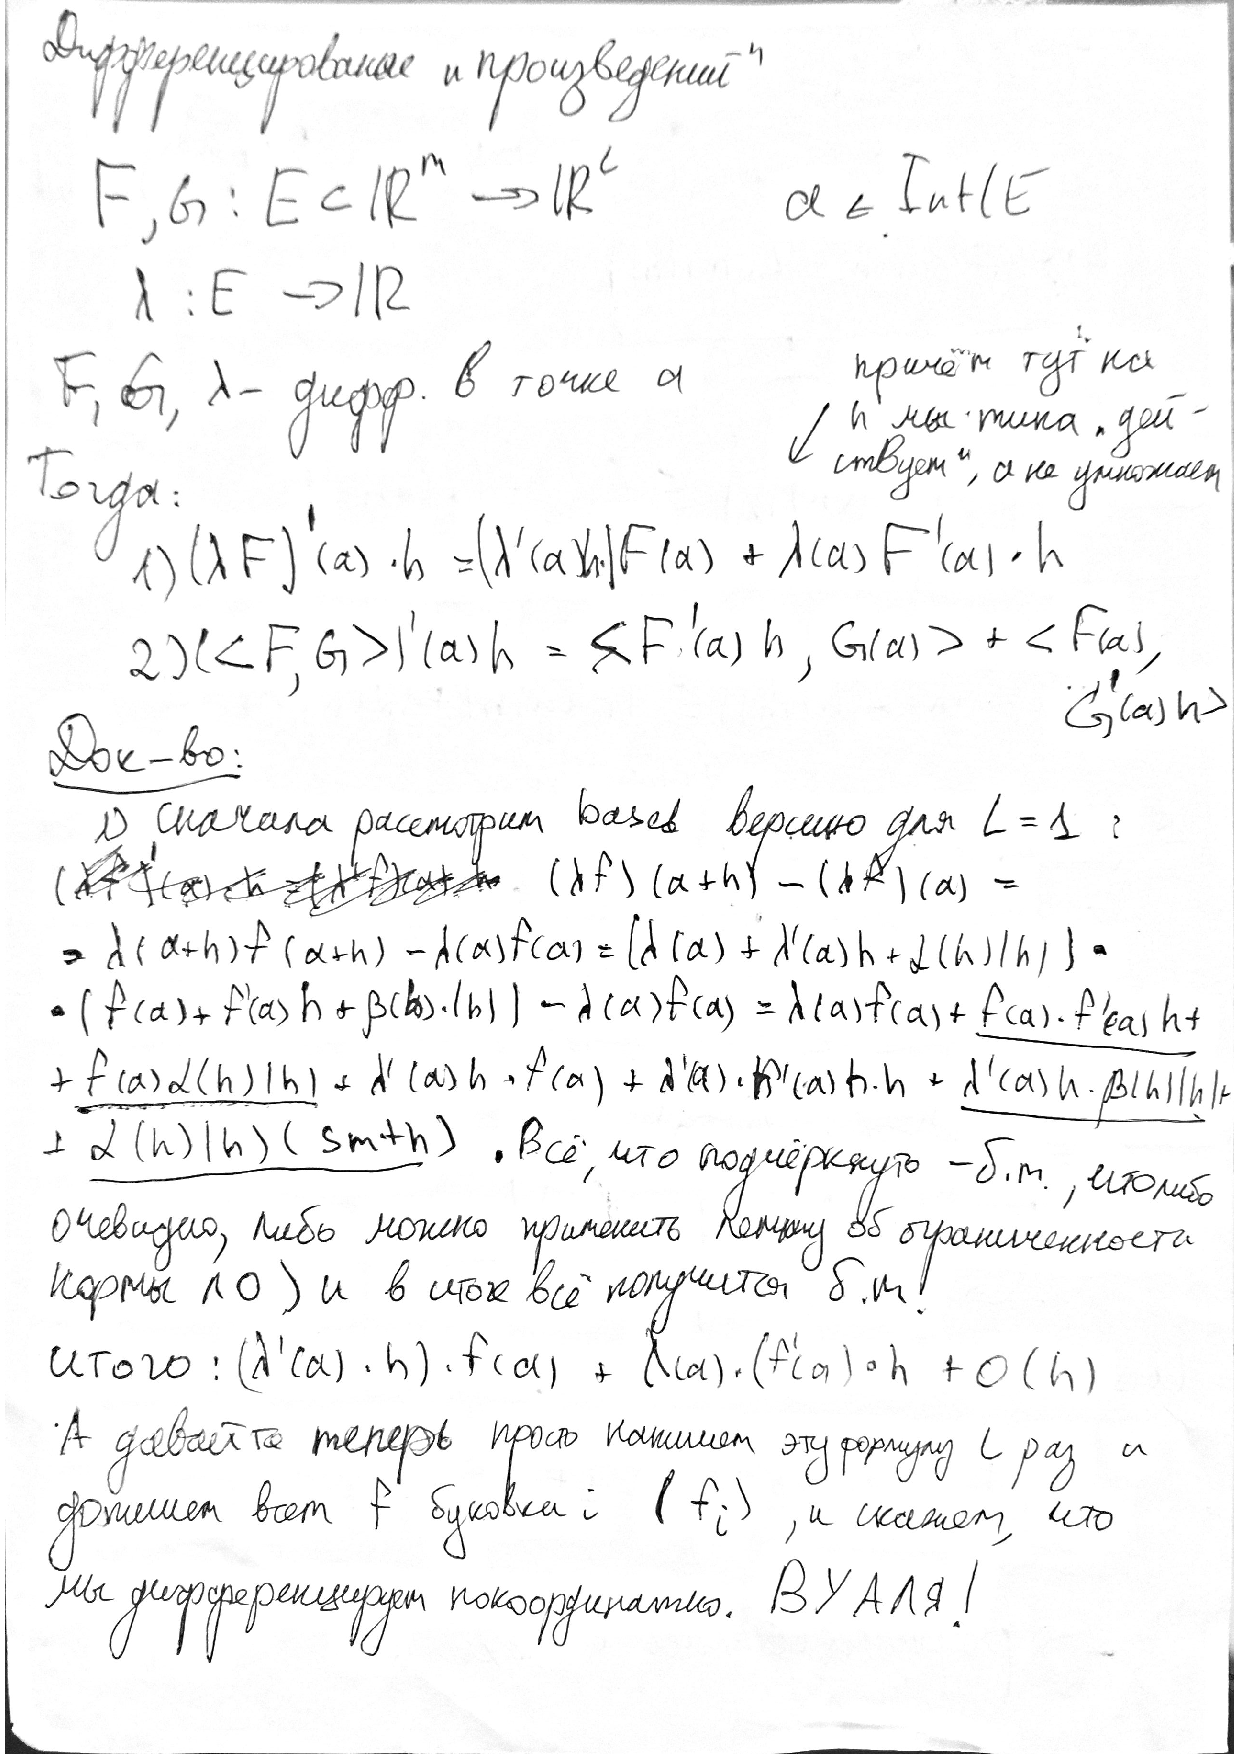
\includepdf[pages={-}]{../images/Dif_mul.pdf}

\subsubsection{Экстремальное свойство градиента\texorpdfstring{$^2$}{}}

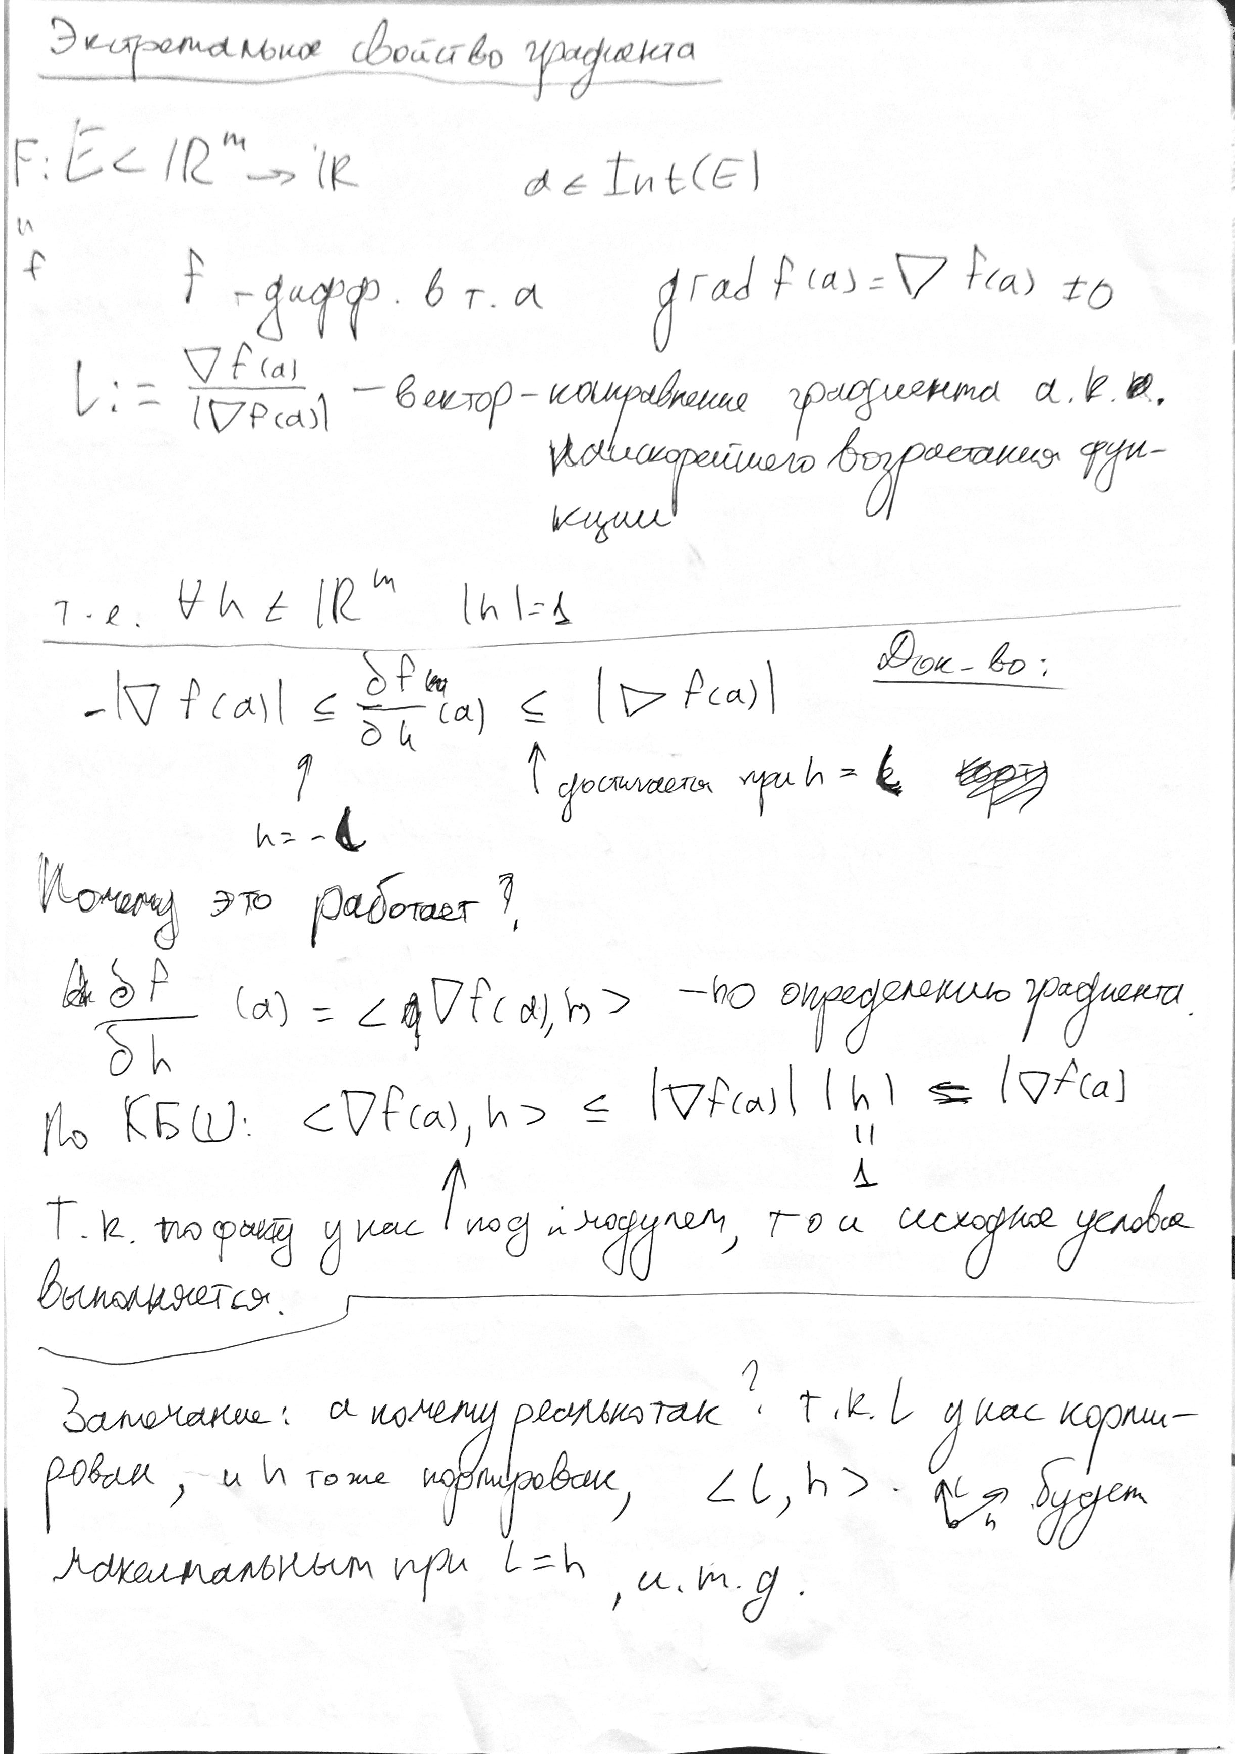
\includepdf[pages={-}]{../images/Extr_Grad.pdf}

\subsubsection{Независимость частных производных от порядка дифференцирования\texorpdfstring{$^2$}{}}

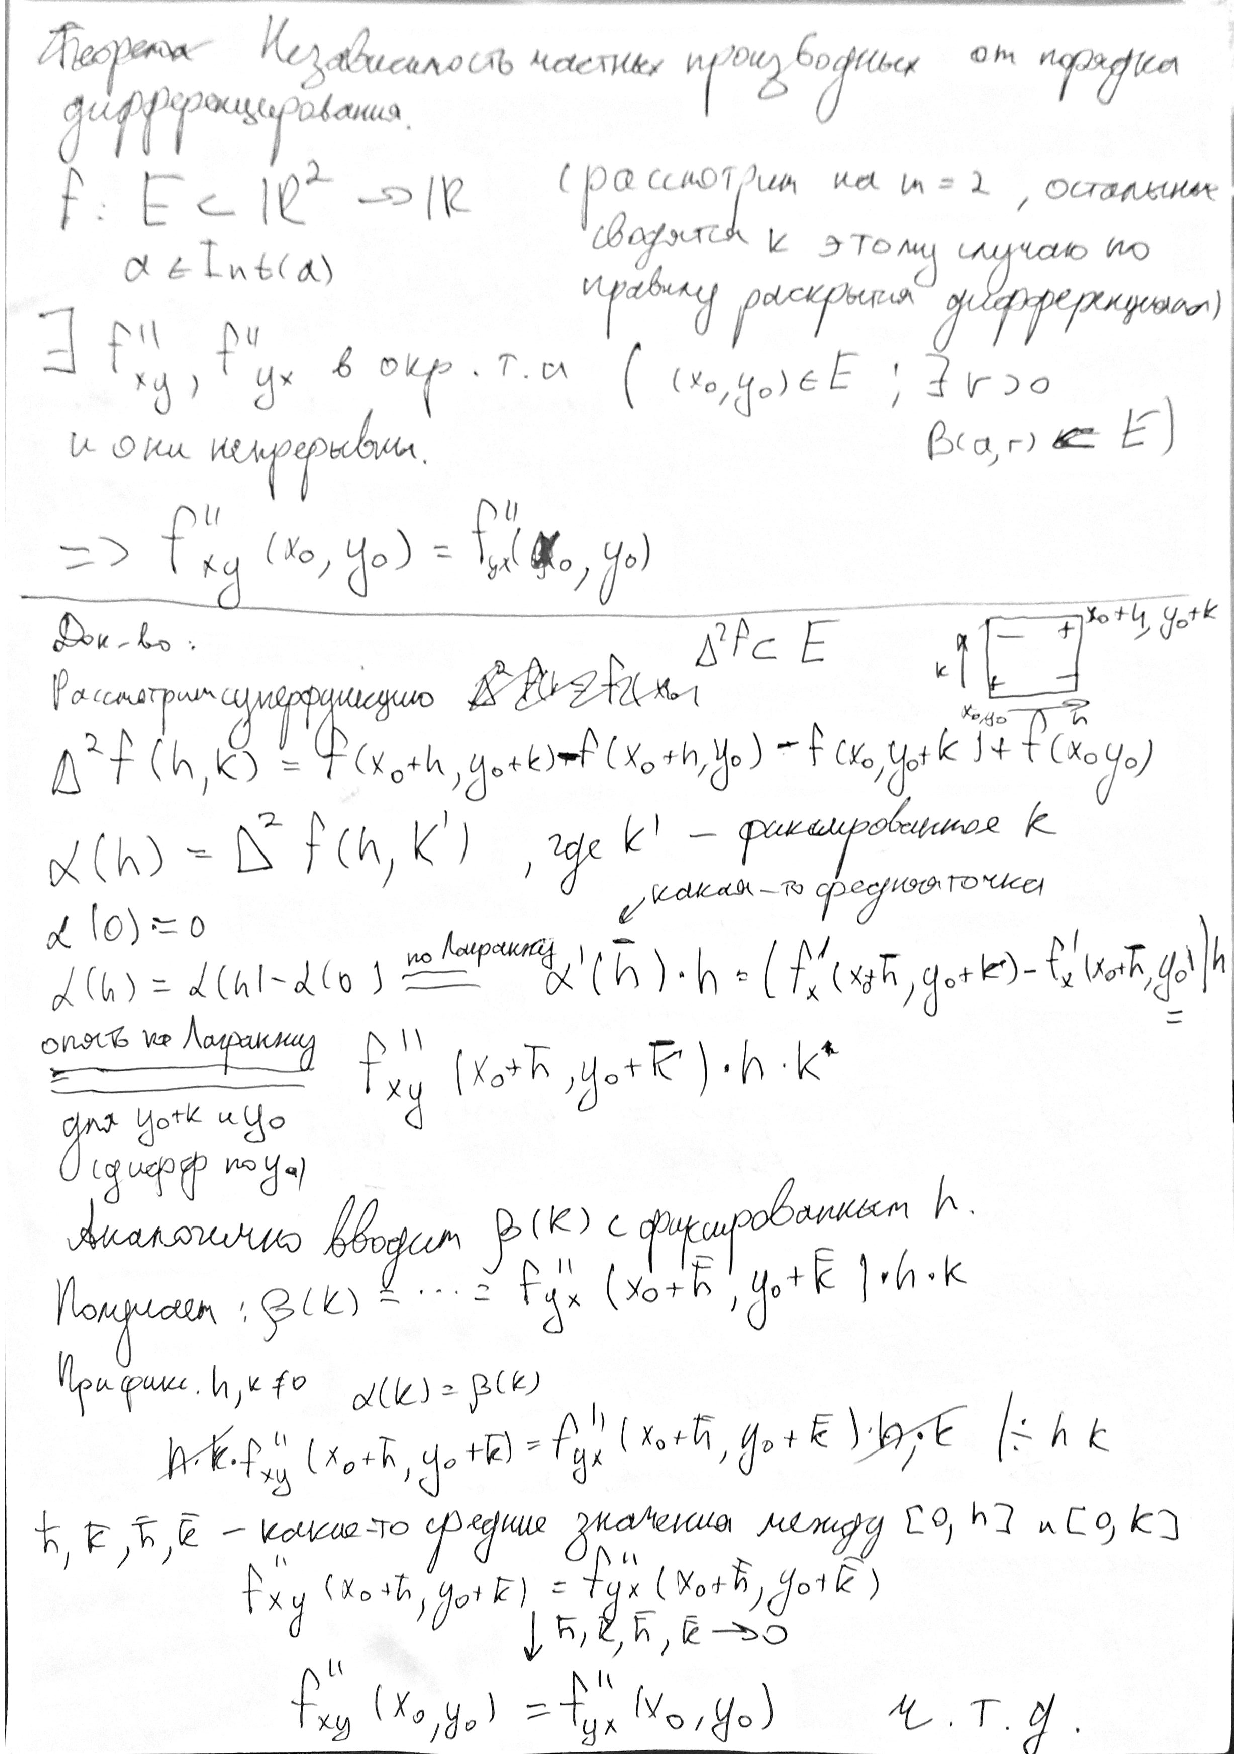
\includepdf[pages={-}]{../images/Nez_Ch.pdf}

\subsubsection{Полиномиальная формула\texorpdfstring{$^2$}{}}

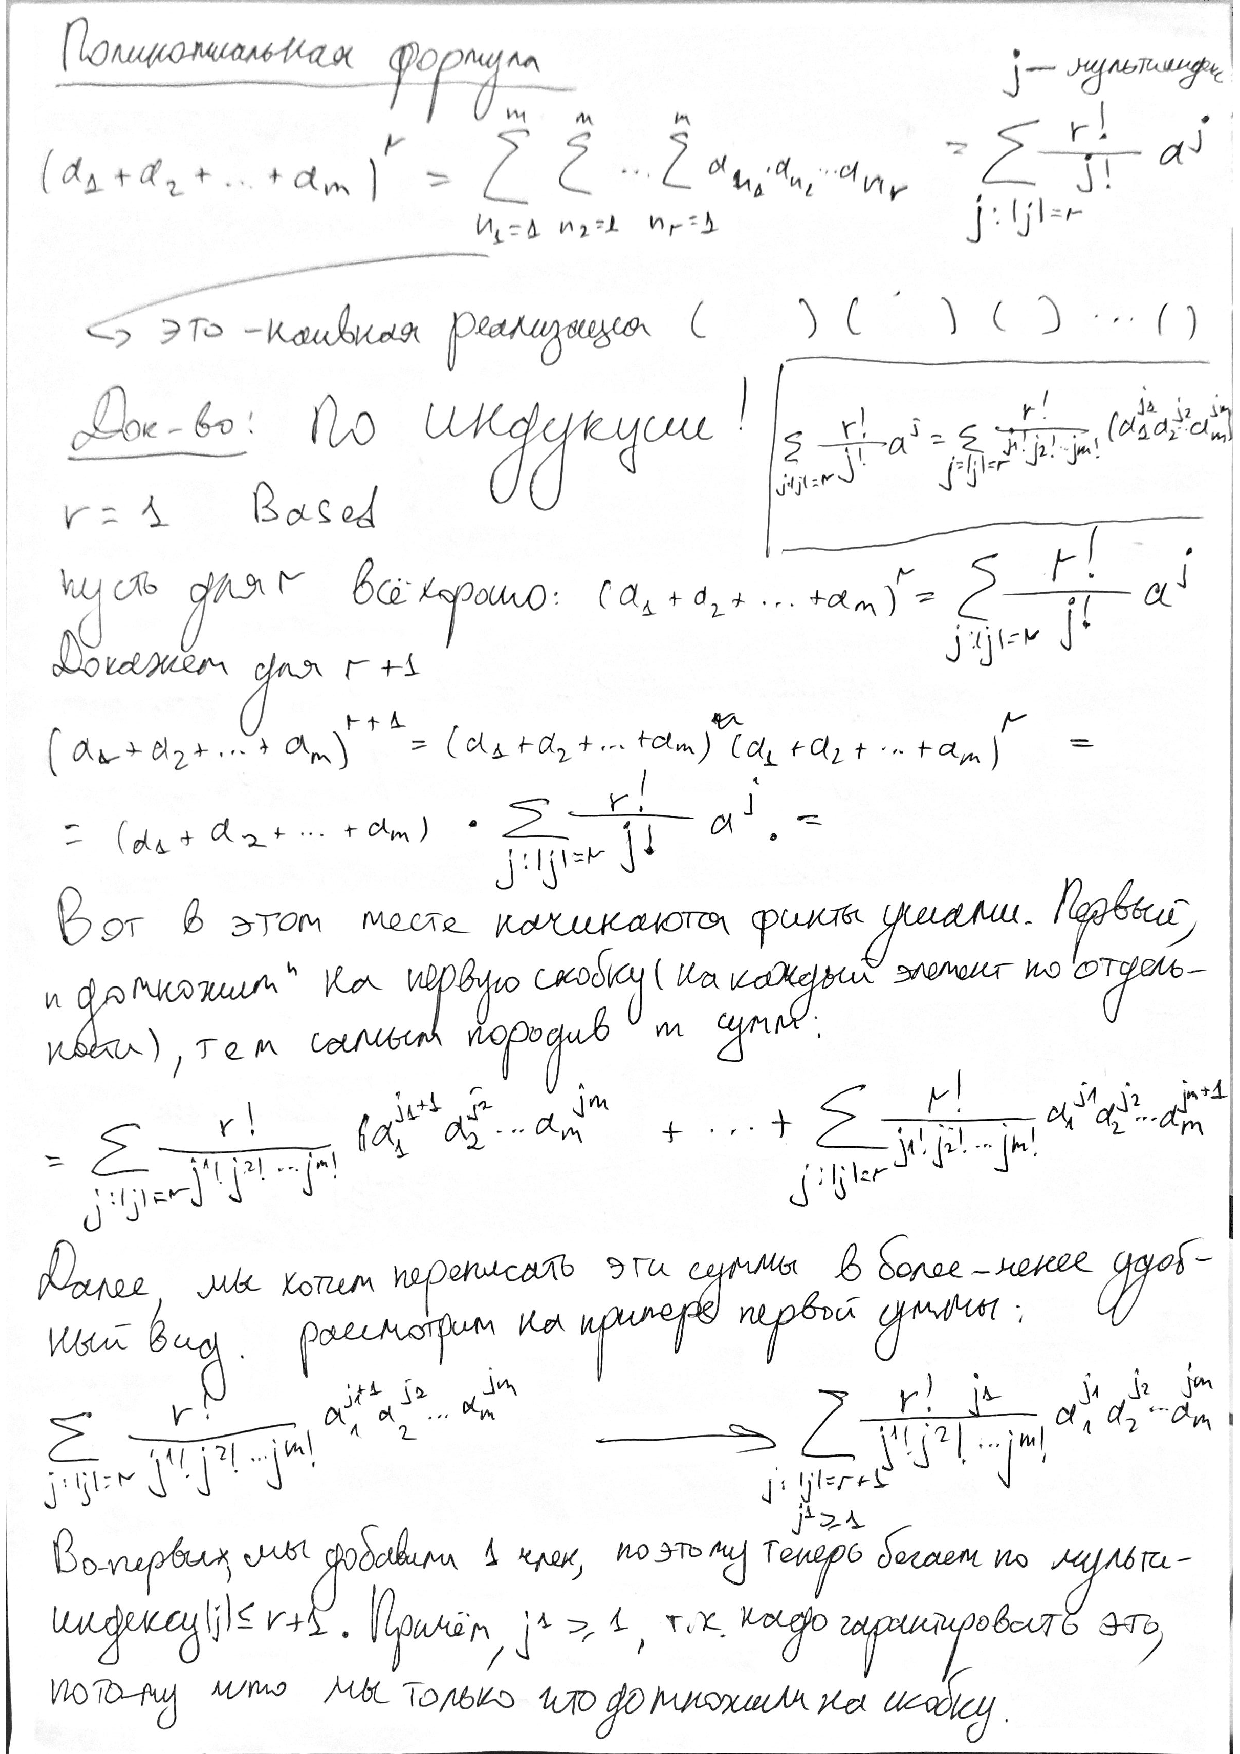
\includepdf[pages={-}]{../images/Polyn_Form.pdf}

\subsubsection{Лемма о дифференцировании "сдвига"\texorpdfstring{$^2$}{}}

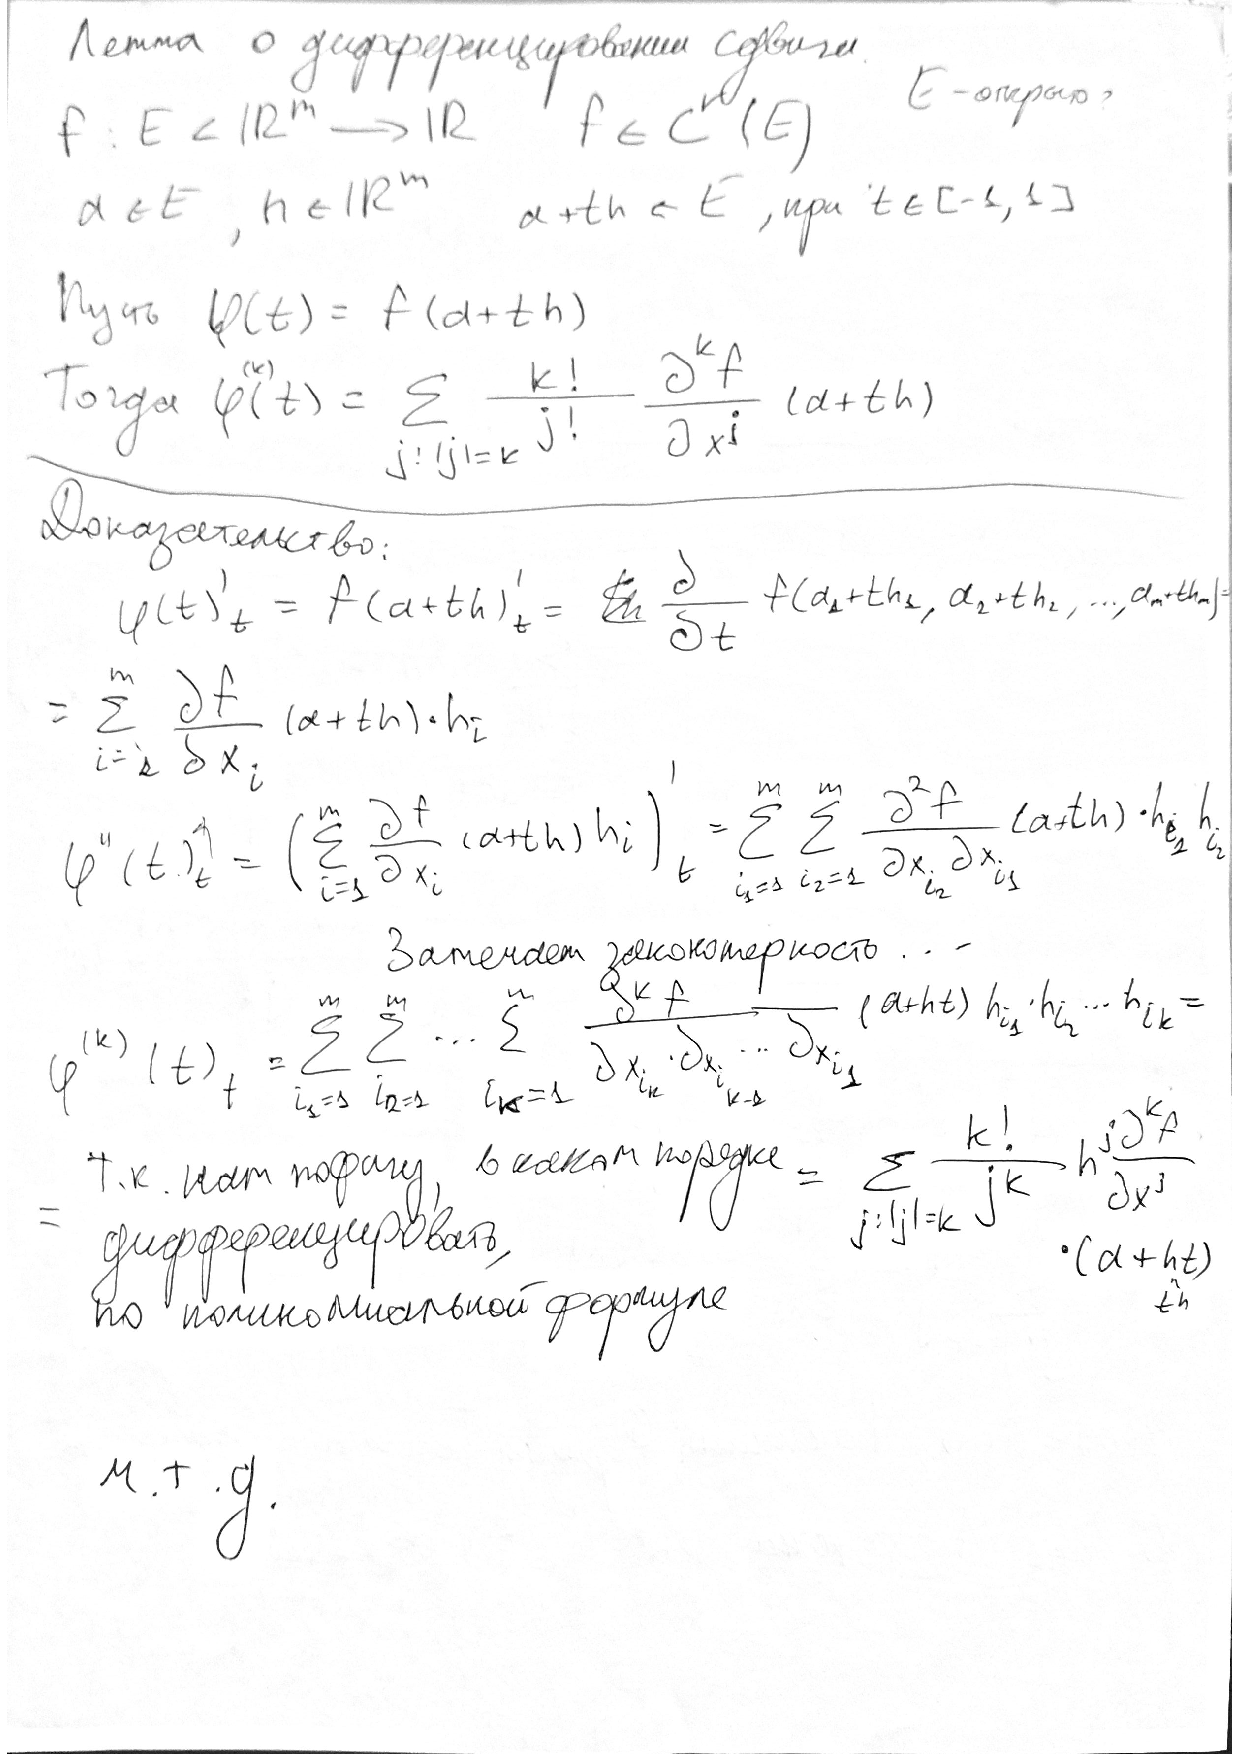
\includepdf[pages={-}]{../images/Lemm_Diff_Sdv.pdf}

\end{document}